%%% Local Variables:
%%% mode: latex
%%% TeX-master: t
%%% End:

%\documentclass[bachelor,nofonts]{thuthesis}
\documentclass[master]{thuthesis}
%\documentclass[doctor]{thuthesis}
% \documentclass[%
%   bachelor|master|doctor|postdoctor, % mandatory option
%   winfonts|nofonts|adobefonts, % mandatory only for bachelor and Linuxer
%   secret,
%   openany|openright,
%   arialtoc,arialtitle]{thuthesis}
% 当使用 XeLaTeX 编译时,本科生、Linux 用户需要加上 nofonts 选项;
% 当使用 PDFLaTeX 编译时,adobefonts 选项等效于 winfonts 选项(缺省选项)。

% 所有其它可能用到的包都统一放到这里了,可以根据自己的实际添加或者删除。
\usepackage{thutils}
\usepackage[table]{xcolor}
\usepackage{algorithm}
\usepackage{algorithmic}
% 你可以在这里修改配置文件中的定义,导言区可以使用中文。
% \def\myname{薛瑞尼}

\begin{document}

% 定义所有的eps文件在 figures 子目录下
\graphicspath{{figures/}}


%%% 封面部分
\frontmatter

%%% Local Variables:
%%% mode: latex
%%% TeX-master: t
%%% End:

% 中国海洋大学研究生学位论文封面
% 参考:中国海洋大学研究生学位论文书写格式20130307.doc

% 为避免出现错误,下面保留[清华大学学位论文模板原有定义无需修改],
% 请直接跳到后面[中国海洋大学学位论文模板部分请根据自己情况修改]。

%%%%%%%%%%%%%%%%%%%%%%[清华大学学位论文模板原有定义无需修改]%%%%%%%%%%%%%%%%%%%%%%%
\secretlevel{绝密} \secretyear{2100}

\ctitle{清华大学学位论文 \LaTeX\ 模板\\使用示例文档}
% 根据自己的情况选,不用这样复杂
\makeatletter
\ifthu@bachelor\relax\else
  \ifthu@doctor
    \cdegree{工学博士}
  \else
    \ifthu@master
      \cdegree{工学硕士}
    \fi
  \fi
\fi
\makeatother


\cdepartment[计算机]{计算机科学与技术系}
\cmajor{计算机科学与技术}
\cauthor{薛瑞尼} 
\csupervisor{郑纬民教授}
% 如果没有副指导老师或者联合指导老师,把下面两行相应的删除即可。
\cassosupervisor{陈文光教授}
\ccosupervisor{某某某教授}
% 日期自动生成,如果你要自己写就改这个cdate
%\cdate{\CJKdigits{\the\year}年\CJKnumber{\the\month}月}

% 博士后部分
% \cfirstdiscipline{计算机科学与技术}
% \cseconddiscipline{系统结构}
% \postdoctordate{2009年7月——2011年7月}

\etitle{An Introduction to \LaTeX{} Thesis Template of Tsinghua University} 
% 这块比较复杂,需要分情况讨论:
% 1. 学术型硕士
%    \edegree:必须为Master of Arts或Master of Science(注意大小写)
%              “哲学、文学、历史学、法学、教育学、艺术学门类,公共管理学科
%               填写Master of Arts,其它填写Master of Science”
%    \emajor:“获得一级学科授权的学科填写一级学科名称,其它填写二级学科名称”
% 2. 专业型硕士
%    \edegree:“填写专业学位英文名称全称”
%    \emajor:“工程硕士填写工程领域,其它专业学位不填写此项”
% 3. 学术型博士
%    \edegree:Doctor of Philosophy(注意大小写)
%    \emajor:“获得一级学科授权的学科填写一级学科名称,其它填写二级学科名称”
% 4. 专业型博士
%    \edegree:“填写专业学位英文名称全称”
%    \emajor:不填写此项
\edegree{Doctor of Engineering} 
\emajor{Computer Science and Technology} 
\eauthor{Xue Ruini} 
\esupervisor{Professor Zheng Weimin} 
\eassosupervisor{Chen Wenguang} 
% 这个日期也会自动生成,你要改么?
% \edate{December, 2005}

% 定义中英文摘要和关键字
\begin{cabstract}
  论文的摘要是对论文研究内容和成果的高度概括。摘要应对论文所研究的问题及其研究目
  的进行描述,对研究方法和过程进行简单介绍,对研究成果和所得结论进行概括。摘要应
  具有独立性和自明性,其内容应包含与论文全文同等量的主要信息。使读者即使不阅读全
  文,通过摘要就能了解论文的总体内容和主要成果。

  论文摘要的书写应力求精确、简明。切忌写成对论文书写内容进行提要的形式,尤其要避
  免“第 1 章……;第 2 章……;……”这种或类似的陈述方式。

  本文介绍清华大学论文模板 \thuthesis{} 的使用方法。本模板符合学校的本科、硕士、
  博士论文格式要求。

  本文的创新点主要有:
  \begin{itemize}
    \item 用例子来解释模板的使用方法;
    \item 用废话来填充无关紧要的部分;
    \item 一边学习摸索一边编写新代码。
  \end{itemize}

  关键词是为了文献标引工作、用以表示全文主要内容信息的单词或术语。关键词不超过 5
  个,每个关键词中间用分号分隔。(模板作者注:关键词分隔符不用考虑,模板会自动处
  理。英文关键词同理。)
\end{cabstract}

\ckeywords{\TeX, \LaTeX, CJK, 模板, 论文}

\begin{eabstract} 
   An abstract of a dissertation is a summary and extraction of research work
   and contributions. Included in an abstract should be description of research
   topic and research objective, brief introduction to methodology and research
   process, and summarization of conclusion and contributions of the
   research. An abstract should be characterized by independence and clarity and
   carry identical information with the dissertation. It should be such that the
   general idea and major contributions of the dissertation are conveyed without
   reading the dissertation. 

   An abstract should be concise and to the point. It is a misunderstanding to
   make an abstract an outline of the dissertation and words ``the first
   chapter'', ``the second chapter'' and the like should be avoided in the
   abstract.

   Key words are terms used in a dissertation for indexing, reflecting core
   information of the dissertation. An abstract may contain a maximum of 5 key
   words, with semi-colons used in between to separate one another.
\end{eabstract}

\ekeywords{\TeX, \LaTeX, CJK, template, thesis}
%%%%%%%%%%%%%%%%%%%%%%%%%%%%%%%%%%%%%%%%%%%%%%%%%%%%%%%%%%%%%%%%%%%%%%%%%%%%%%%%

%%%%%%%%%%%%%%%%%%[中国海洋大学学位论文模板部分请根据自己情况修改]%%%%%%%%%%%%%%%%%%%
% 中国海洋大学研究生学位论文封面
% 必须填写的内容包括(其他最好不要修改):
%   分类号、密级、UDC
%   论文中文题目、作者中文姓名
%   论文答辩时间
%   封面感谢语
%   论文英文题目
%   中文摘要、中文关键词
%   英文摘要、英文关键词
%
%%%%%[自定义]%%%%%
\newcommand{\fenleihao}{}%分类号
\newcommand{\miji}{}%密级 
                    % 绝密$\bigstar$20年 
                    % 机密$\bigstar$10年
                    % 秘密$\bigstar$5年
\newcommand{\UDC}{}%UDC
\newcommand{\oucctitle}{图像中环结构特征及其应用}%论文中文题目
\ctitle{图像中环结构特征及其应用}%必须修改因为页眉中用到
\cauthor{***}%可以选择修改因为仅在 pdf 文档信息中用到
\cdegree{工学博士}%可以选择修改因为仅在 pdf 文档信息中用到
\ckeywords{环结构特征, 图论, 视网膜图像配准, 扇贝图像识别}%可以选择修改因为仅在 pdf 文档信息中用到
\newcommand{\ouccauthor}{***}%作者中文姓名
%\newcommand{\ouccsupervisor}{姬光荣教授}%作者导师中文姓名
%\newcommand{\ouccdegree}{博\hspace{1em}士}%作者申请学位级别
%\newcommand{\ouccmajor}{海洋信息探测与处理}%作者专业名称
%\newcommand{\ouccdateday}{\CJKdigits{\the\year}年\CJKnumber{\the\month}月\CJKnumber{\the\day}日}
%\newcommand{\ouccdate}{\CJKdigits{\the\year}年\CJKnumber{\the\month}月}
\newcommand{\oucdatedefense}{}%论文答辩时间
%\newcommand{\oucdatedegree}{2009年6月}%学位授予时间
\newcommand{\oucgratitude}{谨以此论文献给我的导师和亲人!}%封面感谢语

\newcommand{\oucetitle}{Cycle strcutural feature in image and its applications}%论文英文题目
%\newcommand{\ouceauthor}{Haiyong Zheng}%作者英文姓名
\newcommand{\oucthesis}{\textsc{OUCThesis}}
%%%%%默认自定义命令%%%%%
% 空下划线定义
\newcommand{\oucblankunderline}[1]{\rule[-2pt]{#1}{.7pt}}
\newcommand{\oucunderline}[2]{\underline{\hskip #1 #2 \hskip#1}}

% 论文封面第一页
%%不需要改动%%
\vspace*{5cm}
{\xiaoer\heiti\oucgratitude

\begin{flushright}
---\hspace*{-2mm}---\hspace*{-2mm}---\hspace*{-2mm}---\hspace*{-2mm}---\hspace*{-2mm}---\hspace*{-2mm}---\hspace*{-2mm}---\hspace*{-2mm}---\hspace*{-2mm}---~\ouccauthor
\end{flushright}
}


\newpage
\mbox{}
\newpage

% 论文封面第二页
%%不需要改动%%
\vspace*{1cm}
\begin{center}
  {\xiaoer\heiti\oucctitle}
\end{center}
\vspace{10.7cm}
{\normalsize\songti
\begin{flushright}
{\renewcommand{\arraystretch}{1.3}
  \begin{tabular}{r@{}l}
    学位论文答辩日期:~ & \oucunderline{1.8em}{\oucdatedefense} \\
    指导教师签字:~ & \oucblankunderline{5cm} \\
    答辩委员会成员签字:~ & \oucblankunderline{5cm} \\
    ~ & \oucblankunderline{5cm} \\
    ~ & \oucblankunderline{5cm} \\
    ~ & \oucblankunderline{5cm} \\
    ~ & \oucblankunderline{5cm} \\
    ~ & \oucblankunderline{5cm} \\
    ~ & \oucblankunderline{5cm} \\
  \end{tabular}
}
\end{flushright}
}

\newpage
\mbox{}
\newpage


% 论文封面第三页
%%不需要改动%%
\vspace*{1cm}
\begin{center}
  {\xiaosan\heiti 独\hspace{1em}创\hspace{1em}声\hspace{1em}明}
\end{center}
\par{\normalsize\songti\parindent2em
本人声明所呈交的学位论文是本人在导师指导下进行的研究工作及取得的研究成果。据我所知,除了文中特别加以标注和致谢的地方外,论文中不包含其他人已经发表或撰写过的研究成果,也不包含未获得~\oucblankunderline{7cm}(注:如没有其他需要特别声明的,本栏可空)或其他教育机构的学位或证书使用过的材料。与我一同工作的同志对本研究所做的任何贡献均已在论文中作了明确的说明并表示谢意。
}
\vskip1.5cm
\begin{flushright}{\normalsize\songti
  学位论文作者签名:\hskip2cm 签字日期:\hskip1cm 年 \hskip0.7cm 月\hskip0.7cm 日}
\end{flushright}
\vskip.5cm
{\setlength{\unitlength}{0.1\textwidth}
  \begin{picture}(10, 0.1)
    \multiput(0,0)(0.2, 0){50}{\rule{0.15\unitlength}{.5pt}}
  \end{picture}}
\vskip1cm
\begin{center}
  {\xiaosan\heiti 学位论文版权使用授权书}
\end{center}
\par{\normalsize\songti\parindent2em
本学位论文作者完全了解学校有关保留、使用学位论文的规定,并同意以下事项:
\begin{enumerate}
\item 学校有权保留并向国家有关部门或机构送交论文的复印件和磁盘,允许论文被查阅和借阅。
\item 学校可以将学位论文的全部或部分内容编入有关数据库进行检索,可以采用影印、缩印或扫描等复制手段保存、汇编学位论文。同时授权清华大学“中国学术期刊(光盘版)电子杂志社”用于出版和编入CNKI《中国知识资源总库》,授权中国科学技术信息研究所将本学位论文收录到《中国学位论文全文数据库》。
\end{enumerate}
(保密的学位论文在解密后适用本授权书)
}
\vskip1.5cm
{\parindent0pt\normalsize\songti
学位论文作者签名:\hskip4.2cm\relax%
导师签字:\relax\hspace*{1.2cm}\\
签字日期:\hskip1cm 年\hskip0.7cm 月\hskip0.7cm 日\relax\hfill%
签字日期:\hskip1cm 年\hskip0.7cm 月\hskip0.7cm 日\relax\hspace*{1.2cm}}

\newpage
\mbox{}
\newpage
\pagestyle{plain}
\clearpage\pagenumbering{roman}

% 中文摘要
%%[需要填写:中文摘要、中文关键词]%%
\begin{center}
  {\sanhao[1.5]\heiti\oucctitle\\\vskip7pt 摘\hspace{1em}要}
\end{center}
{\normalsize\songti

  \indent
  近年来,随着计算机视觉领域的不断发展,特征提取作为最重要的一环得到了大量学者的重视和研究。局部特征可把繁杂的图像匹配的问题转换为特征向量的度量问题,可以大大减小算法的复杂度,因而获得了迅速发展。本文针对存在环结构特征的图像,提出了一种环结构局部不变特征,满足平移、缩放、旋转不变性,可应用于图像识别、图像配准等各个领域。本文的主要工作有:
\begin{enumerate}
\item 环结构特征提取与描述。结合图论中环的概念,实现了在图像中提取及描述环结构特征,即先用多尺度分割算法与骨架化算法提取图像中的分叉点或交叉点及它们之间的连线,滤除不能组成环结构的特征点,从而找到特征点之间的连接关系。应用我们提出的动态路径移动算法检测环结构,并用归一化的分叉角度与分支长度来把环结构描述成特征向量。

\item 基于环结构特征的视网膜图像配准。实现了把环结构特征应用于视网膜图像配准中,即在得到环结构特征向量后,用相似性度量进行特征向量匹配,找到最匹配的环结构特征对,用相似性变换把一幅图像变换到另一幅图像中。提出骨架化对准精度来对配准结果进行定量评估。本文用VARIA数据集中的153对视网膜图像进行实验,配准成功率高达96.73\%,骨架化对准精度为0.938。论文中还给出了不同变换模型、不同特征之间的实验对比,以此来说明用环结构来做视网膜图像配准的可行性和有效性。

\item 基于环结构特征的扇贝图像识别。构建了扇贝图像识别图像库,包括标准图像库与待识别图像库,并通过相似性度量进行特征匹配。根据得到的最匹配的环结构特征对找到标准图像库中与待识别图像库中相对应的扇贝图像,以此来达到识别的目的。针对构建的图像识别数据库,实验成功率达到83.3\%,说明用环结构特征来进行扇贝图像识别是可行且有效的。

\end{enumerate}

本文提出了环结构局部不变特征,并在视网膜图像配准与扇贝图像识别等领域都得到了成功应用,具有十分重要的意义。

}
\vskip12bp
{\xiaosi\heiti\noindent
关键词:\hskip1em 环结构特征; 图论; 视网膜图像配准; 扇贝图像识别}

\newpage
\mbox{}
\newpage
% 英文摘要
%%[需要填写:英文摘要、英文关键词]%%
\begin{center}
  {\sanhao[1.5]\heiti\oucetitle\\\vskip7pt Abstract}
\end{center}
{\normalsize\songti
With the development of computer vision, feature extraction, as one of the most important technique, has got a lot of attention and research in recent years. Local features convert the complicated matching problem to the measure of feature vectors, can greatly reduce the complexity of the algorithm. The cycle structural features based on the images with cycles can be applied to image recognition and registration as they are invariant to translation, scaling and rotation. The main work of this paper includes:

\begin{enumerate}
\item Extraction and description of cycle structural feature. According to the concept of cycle in graph, the algorithm to extract and descript cycle structural feature in images is proposed. Multiscale segmentation method and skeleton method are applied to obtain the bifurcations or intersections and the lines connected with them in images firstly. Dynamic path moving algorithm is proposed to detect the cycle structural features under the premise that the invalid points are filtered and the connection between points are detected. Finally, the angles and lengths of the branches are used to describe the cycle to feature vectors. 
\item Retinal image registration based on cycle structural features. After the feature vectors obtained, using the similarity measure to match and find the best matching pair. The similarity transformation is used to transform one image to another according to the best matching pair to reach the purpose of registration. The VARIA database which includes 153 pairs of retinal images is used in this paper to verify the effectiveness and feasibility of the algorithm.
In order to evaluate the result quantitiatively, the Skeleton Alignment Error Measure (SAEM) is calculated and the final registration result is 0.938.
\item Scallop image recognition based on cycle structural features. The scallop image recognition database is built which includes standard image database and image database used to be recognized. The similarity measure is applied to match the feature vectors and the corresponding images between these two databases can be found according to the best matching pairs. For the built scallop image recognition database, the recognition success rate reached to 83.3\%, which means this method is feasible and effective for recognition purpose.
\end{enumerate}  	
The cycle structural feature is proposed in this paper and applied in the retinal image registration and scallop image registration, which means it has very vital significance.
   
}
\vskip12bp
{\xiaosi\heiti\noindent 
\textbf{Keywords:\enskip cycle structural feature, graph theory, retinal image registration, scallop image recognition}}
%%%%%%%%%%%%%%%%%%%%%%%%%%%%%%%%%%%%%%%%%%%%%%%%%%%%%%%%%%%%%%%%%%%%%%%%%%%%%%%%

% 设置 PDF 文档的作者、主题等属性
\makeatletter
\thu@setup@pdfinfo
\makeatother
%\makecover

% 目录
\tableofcontents

% 符号对照表
%\begin{denotation}

\item[HPC] 高性能计算 (High Performance Computing)
\item[cluster] 集群
\item[Itanium] 安腾
\item[SMP] 对称多处理
\item[API] 应用程序编程接口
\item[PI]	聚酰亚胺
\item[MPI]	聚酰亚胺模型化合物,N-苯基邻苯酰亚胺
\item[PBI]	聚苯并咪唑
\item[MPBI]	聚苯并咪唑模型化合物,N-苯基苯并咪唑
\item[PY]	聚吡咙
\item[PMDA-BDA]	均苯四酸二酐与联苯四胺合成的聚吡咙薄膜
\item[$\Delta G$]  	活化自由能~(Activation Free Energy)
\item [$\chi$] 传输系数~(Transmission Coefficient)
\item[$E$] 能量
\item[$m$] 质量
\item[$c$] 光速
\item[$P$] 概率
\item[$T$] 时间
\item[$v$] 速度
\item[劝  学] 君子曰:学不可以已。青,取之于蓝,而青于蓝;冰,水为之,而寒于水。
  木直中绳。(车柔)以为轮,其曲中规。虽有槁暴,不复挺者,(车柔)使之然也。故木
  受绳则直, 金就砺则利,君子博学而日参省乎己,则知明而行无过矣。吾尝终日而思
  矣,  不如须臾之所学也;吾尝(足齐)而望矣,不如登高之博见也。登高而招,臂非加
  长也,  而见者远;  顺风而呼,  声非加疾也,而闻者彰。假舆马者,非利足也,而致
  千里;假舟楫者,非能水也,而绝江河,  君子生非异也,善假于物也。积土成山,风雨
  兴焉;积水成渊,蛟龙生焉;积善成德,而神明自得,圣心备焉。故不积跬步,无以至千
  里;不积小流,无以成江海。骐骥一跃,不能十步;驽马十驾,功在不舍。锲而舍之,朽
  木不折;  锲而不舍,金石可镂。蚓无爪牙之利,筋骨之强,上食埃土,下饮黄泉,用心
  一也。蟹六跪而二螯,非蛇鳝之穴无可寄托者,用心躁也。\pozhehao{} 荀况
\end{denotation}



%%% 正文部分
\mainmatter

%%% Local Variables:
%%% mode: latex
%%% TeX-master: t
%%% End:

\chapter{绪论}
\label{cha:intro}


\section{引言}
\label{}

近年来,随着计算机视觉领域的不断发展,特征提取作为最重要的一环也得到了大量学者的重视和研究\cite{shipeng}。在计算机视觉发展初期,人们往往通过直方图等全局特征来获取整幅图像的信息\cite{liuying},然而,全局特征对于有部分遮挡、背景杂乱的图像具有很强的敏感性。于是,这就刺激了研究人员对局部特征的研究。局部特征主要利用图像中显著的局部信息来描述图像,局部特征可能是点、边缘、或者区域,通过特征检测技术和特征描述技术将局部特征描述为特征向量,就可把繁杂的图像匹配的问题转换为特征向量的度量问题,这样就能大大减小算法的复杂度,提高算法的有效性。好的局部特征应该满足几个属性:首先,对于从不同角度,不同时间拍摄的图像,应能保证局部特征的有效和不变性,其次,局部特征与图像背景之间应该有较大差异,能够方便和准确的进行提取,最后,局部特征应具有一定的数量,以便能够在图像中检测足够多的特征进行应用。

局部不变特征的这些属性决定了其在计算机视觉各个领域能得到广泛应用,比如在图像识别、图像配准、目标跟踪、图像检索、图像拼接等领域都需要局部特征的提取、描述与匹配。

本文提出了一种新的局部不变特征,即环结构特征,以应用于图像中存在环结构特征的各类图像,比如建筑物图像、树叶图像、视网膜图像、扇贝贝壳图像等。环结构特征由图像中存在的交叉、分叉点及它们之间的连线构成,用归一化的连线长度及分叉角度等信息将环结构描述成特征向量,可满足平移、缩放、旋转不变性,因此可应用于图像识别、图像配准等各个领域。


\section{国内外研究现状}
\label{} 



\subsection{图像中局部不变特征的研究现状}
\label{}

局部特征就是从图像的局部区域出发,用显著的局部信息来构造出具有稳定性的描述子。局部特征描述了图像局部区域的信息,由于图像各个区域之间存在像素、颜色或纹理等方面的差异,局部特征体现出了唯一性。近些年来,计算机视觉领域获得迅猛发展,局部特征技术也引起了足够的重视,很多学者纷纷加入研究,越来越多的局部特征描述子在图像配准、物体识别、图像检索等领域获得了大量的应用。

Harris角点特征检测方法\cite{harris}是经典的局部特征检测算法,Harris算法是由Moravec\cite{moravec}算法发展而来,Morave角点检测公式如式\ref{eq:morave},其中$w(x, y)$是高斯平滑因子,种子像素点$I(x, y)$平移$(u, v)$窗口后的灰度变化为E:

\begin{align}
E(u, v)|_{(x, y)} = \sum_{x, y}w(x, y)[I(x + u, y + v) - I(x, y)]^2 
\label{eq:morave}
\end{align}
上式中。基于Morave算法,Harris提出了新的改进,为了抑制噪声,对图像进行了平滑处理。将式\ref{eq:morave}进行泰勒级数展开,得到:
\begin{align}
E(u, v)|_{(x, y)} \doteq [u, v]M\left[ \begin{array}{l}
u \\
v
\end{array} \right]
\end{align}
\begin{align}
M = \sum_{x, y} w(x, y)\left[ \begin{array}{ll}
I_x^2 & I_xI_y\\
I_xI_y & I_y^2
\end{array} \right]
\end{align}
上式中忽略了泰勒级数的高阶项,$I_x$和$I_y$分别为种子像素点在x和y方向上的导数。将M做相似对角化处理,得到:
\begin{align}
M \to R^{-1}\left[ \begin{array}{ll}
\lambda_1 & \\
 & \lambda_2
\end{array} \right]R
\end{align}
其中,$\lambda_1, \lambda_2$是M的特征值,R为旋转因子。Harris的核心思想是:在水平、竖直两个方向上变化均较大的点为角点,即此时两个特征值都比较大,仅在水平或垂直一个方向有较大的变化量为边缘点,即此时有一个特征值较大,当在水平、竖直两个方向的变化量都较小,即两个特征值都相对较小时为平滑区域。这个核心思想可表示为:
\begin{align}
\left\{ \begin{array}{l}
\textrm{Corness = detM - $k(traceM)^2$} \\
\textrm{detM = $\lambda_1\lambda_2$} \\
\textrm{traceM = $\lambda_1 + \lambda_2$}
\end{array} \right.
\end{align}
其中,k是一个经验值,当检测到Corness大于某一设定值且为局部极值点时,可认为是角点。

文献\cite{yezhiyong}认为Harris角点检测算法需要合适的阈值来检测理想的特征点,而阈值的获取依靠大量的实验才能确定,选取不合适则会造成聚类现象的产生。且文献\cite{zhangyong}认为Harris对噪声敏感,对特征点的定位不够准确。

Lowe提出一种具有尺度不变的局部特征,即SIFT算子\cite{lowe}。该方法将图像与不同高斯尺度的变换核相卷积,得到不同尺度下的图像。该算法即使在图像缩放尺度比较大的情况下,也能稳定可靠的提取特征点,且对光照具有一定的适应性。二维搞死卷积核如下:
\begin{align}
G(x, y, \sigma) = \frac{1}{2\pi\sigma^2}e^{-(x^2+y^2)/2\sigma^2}
\end{align}
其中,$\sigma$表示高斯函数分布的方差,不同尺度的图像可表示为:
\begin{align}
L(x, y, \sigma) = G(x, y, \sigma) \otimes I(x, y)
\end{align}

$L(x, y, \sigma)$表示尺度为$\sigma$的图像,$\sigma$表示尺度因子,用来控制图像平滑的程度,$\sigma$越大表示图像平滑的越大。

除此之外,国内外还提出了很多优秀的局部特征描述子,比如Hessian,Susan\cite{smith},SURF\cite{bay}算法等等,这些算子都是比较通用的算法,可以针对不同种类的图像加以应用,但针对某一类图像,可能效果不是很理想。本文提出了一种新的稳定的局部不变特征,即环结构特征,以应用于图像中存在环结构特征的各类图像,将其描述成特征向量,用于图像识别、图像配准等领域。由于环结构特征更具有针对性,故而应用于图像中存在环结构的各类图像,效果更加理想。

\subsection{环结构特征的研究现状}
\label{sec:complicatedtable}

环结构是图论中的概念。在人类社会的实际生活中,有时在描述某些事物或对象之间有某种特定关系时采用图形的方式显得更加直观。对象用图形中的点表示,两对象之间具有的某种特定的关系用两点之间的无向或有向连线表示,由此数学抽象产成了图的概念\cite{xujunming}。环在图论中表示一系列边的集合,起始点与终止点是重合的。

在图中检测最小环是图中的研究的最基本的问题。针对这个问题已有很多方面的应用及研究。比如电路测试、结构工程、计算机程序频率分析、有机化学中的复杂合成等各个方面。国内外学者针对检测最小环的问题提出了很多算法。

Mateti和Deo\cite{mateti},Syslo\cite{syslo}提出了检测图中的简单环的算法,Dixon和Goodman\cite{goodman}提出了寻找最长环的算法。Chua和Chen提出把寻找环的问题应用于电路网络中\cite{chua}。上述算法中,工作量大都取决于所选择的环基。若一个环基中所包含的是最小环,则能加快算法的速度,这就刺激了一些学者开始研究检测最小环的算法。最初,Stepanec和Zykov提出了检测最小环的算法\cite{stepanec},Hubicka和Syslo\cite{hubicka}提出,Stepanec的算法不适用于所有的图,并提出了自己的算法。但Kolasinska\cite{kola}给出了一个Hubicka检测最小环基失败的案例。Steeves提出了一种不同的算法,但仍有失败的案例。Deo,Prabhu和Krishnamoorthy\cite{deo}提出这个问题是个N-P问题。

第一个提出多项式时间算法来解决检测最小环基问题的是Horton\cite{horton},复杂度是$O(m^3n)$,de Pina\cite{pina}提出了一个不同的$O(m^3+mn^2logn)$的算法,Golynski和Horton\cite{golynski}通过利用快速矩阵乘法改进了Horton的算法,复杂度为$O(m_{\omega}n)$,$\omega \le 2.376$。Berger\cite{berger}利用与de Pina相同的思想提出了一个复杂度为$O(m^3+mn^2logn)$的算法。Kavitha\cite{kavitha}等人改进了Pina的算法,复杂度为$O(m^2n+mn^2logn)$。Mehlhorn\cite{mehlhorn}提出了一种复杂度为$O(m^2n^2)$的混合算法,之后又基于最小反馈点集提出$O(m^2n)$的算法,最终又改进到$O(m^2n/logn + mn^2)$。

这些算法都是用于解决图论中的问题,为了在图像中能够检测最小环,我们提出了动态路径移动算法。我们首先检测了图像中的分叉结构作为特征点,然后根据特征点之间的连接关系检测环结构,实验证明利用动态路径移动算法能成功的检测到图像中的环结构。

\section{课题背景}
\label{sec:theorem}

本课题主要受国家自然科学基金项目“基于视觉注意结合生物形态特征的海洋浮游植物显微图像分析(编号:61301240)”与“基于形态特征的中国海常见有害赤潮藻显微图像识别(编号:61271406)”资助。


\section{主要工作及内容安排}
\label{sec:bib}

本文的主要工作如下:

第一章为绪论,主要介绍了局部不变特征的相关知识及国内外研究现状、图论中环结构检测的主要研究现状、课题来源以及本文的主要工作和内容安排等。

第二章介绍了环结构特征的定义、特点及应用,以及如何在图像中提取和描述环结构特征。提出了提取及描述环结构的主要步骤,即先用多尺度分割算法与骨架化算法提取图像中的点与线,滤除不能组成环结构的特征点,从而找到特征点之间的连接关系。应用我们提出的动态路径移动算法检测环结构,并用分叉角度与分支长度来把环结构描述成特征向量。

第三章主要把环结构特征应用于视网膜图像配准中。介绍了近年来视网膜配准的研究现状,并阐述了如何把环结构特征向量应用在图像配准中,即用相似性度量进行特征向量匹配,再用相似性变换把一幅图像变换到另一幅图像中。提出了首先使用环上的分叉点及与环相连的血管点来做初始全局配准,再用局部未配准分叉点进行局部纠正的策略,并给出了具体步骤。同时,还给出了不同变换模型、不同特征、不同方法之间的实验对比,以此来说明用环结构来做视网膜图像配准的可行性和有效性。

第四章主要介绍如何把环结构特征用于扇贝图像识别上。介绍了国内外扇贝图像识别的研究现状,构建了扇贝图像识别图像库,并用环结构进行实验来说明用环结构来进行扇贝图像识别的有效性。

第五章是对本论文工作的分析总结以及对今后所要进行工作的展望。


%%% Local Variables: 
%%% mode: latex
%%% TeX-master: t
%%% End: 

\chapter{环结构特征}
\label{cha:cycle}



本文提出了一种新的局部不变特征,即环结构特征,以应用于图像内容中存在环结构特征的各类图像,比如建筑物图像、树叶图像、视网膜图像、扇贝贝壳图像等。基本流程如图\ref{fig:Example}所示,环结构特征由图像中存在的交叉、分叉点及它们之间的连线构成,建筑物中的水泥框架、树叶中的叶脉、视网膜中的血管、扇贝贝壳纹理都可以形成环结构。通过将环结构描述成特征向量,即可应用于识别、配准等各个领域。

\begin{figure}[H]
\centering
  \begin{minipage}[b]{0.48\textwidth} 
      \centering 
      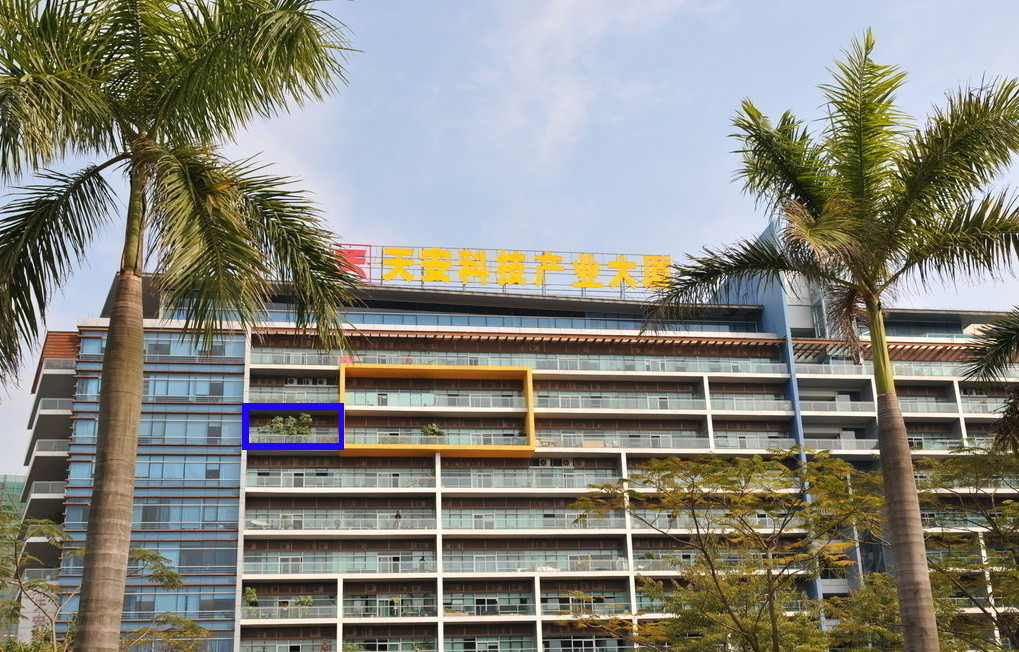
\includegraphics[width=5cm]{chap02/building}
        \centerline{(a) 建筑物}\medskip
    \end{minipage}
  \begin{minipage}[b]{0.48\textwidth}
    \centering
    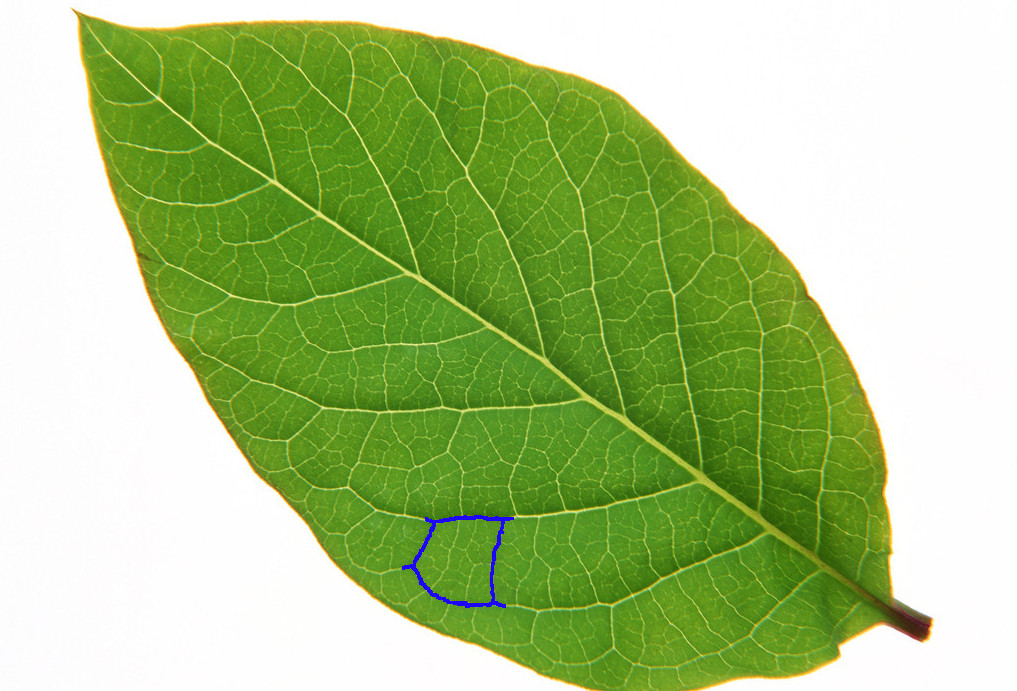
\includegraphics[width=5cm]{chap02/reaf}
      \centerline{(b) 树叶}\medskip
  \end{minipage}
  \begin{minipage}[b]{0.48\textwidth}
    \centering
    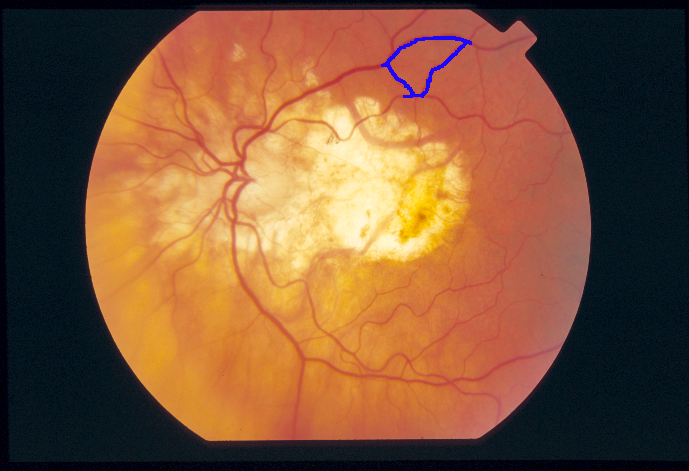
\includegraphics[width=5cm]{chap02/retinal}
      \centerline{(c) 视网膜}\medskip
  \end{minipage}
  \begin{minipage}[b]{0.48\textwidth}
    \centering
    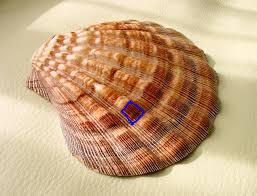
\includegraphics[width=5cm]{chap02/scallop}
      \centerline{(d) 扇贝}\medskip
  \end{minipage}
\caption{图像中的环结构}
\label{fig:Example}
\end{figure}




\section{预处理}
\label{}

原始图像一般都是灰度或彩色图像,若想从中提取环结构来用做识别或配准的特征,需要对其进行预处理,以使得环结构特征更加突出,以便能够准确快速的提取。对于原始图像的预处理主要分为四步,即基于偏微分方程的多尺度图像分割、连通区域标记图像去噪、膨胀腐蚀操作填充孔洞、骨架化,如图\ref{fig:Preprocessing}所示。经过这四步处理,原始图像转化为骨架化后的二值图像,以便进行环结构特征的提取。
\begin{figure}[H]
\centering
    \centering
    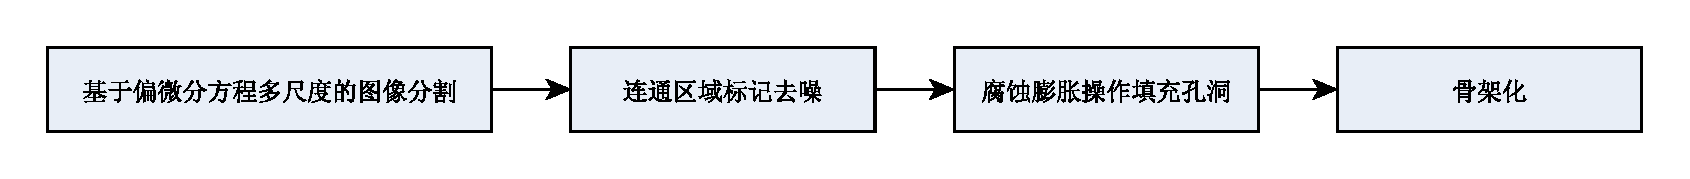
\includegraphics[width=13cm]{chap02/preprocessing}\medskip
\caption{预处理流程图}
\label{fig:Preprocessing}
\end{figure}
\subsection{基于偏微分方程的多尺度图像分割}

图像分割是计算机视觉领域的至关重要的技术,是介于图像分析与低层图像处理之间的图像处理过程,因而图像分割的结果好坏将很大程度上影响后续对图像的处理及应用。近些年来,对图像分割技术的研究层出不穷,分为基于区域的分割,基于边缘的分割,基于特定理论的分割,如基于模糊理论的分割、基于水平集的分割、基于活动轮廓的分割、基于图论的分割\cite{xuxiaoli}等等。

环结构特征存在于很多类图像中,不同类图像的环结构之间有很大的不同。例如,视网膜血管图像中血管较细、直径宽度变化范围大,血管与背景对比度低,扇贝贝壳纹理图像中边缘较模糊等,这就增加了图像分割的难度。为了减小图像分割对图像配准或识别的影响,并且使分割结果能够适用于多类不同图像,我们采用了基于偏微分方程多尺度的图像分割。

基于偏微分方程的多尺度图像分割\cite{wang2013retinal}不需要预处理与训练,可直接用于各类图像的分割。首先,利用多小波核对不同边缘的反映特性的不同,对图像中的边缘进行增强。通过多尺度多层分解方法对归一化的图像进行处理,以达到去除噪声和定位边缘的目的。尺度不同表示边缘的细化程度不同。最后,采用自适应阈值方法得到分割后的二值图像,图\ref{fig:flow-segmentation}为基本流程图。这样一幅图像就得到了不同尺度的多个分割结果,针对不同的应用问题就可以选择不同的尺度进行后续处理。

\begin{figure}[H]
\centering
    \centering
    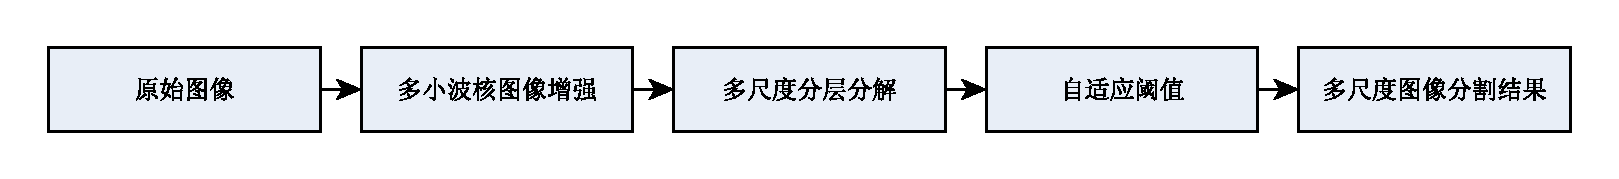
\includegraphics[width=13cm]{chap02/flow-chart-segmentation}\medskip
\caption{多尺度图像分割流程图}
\label{fig:flow-segmentation}
\end{figure}

二维多小波核$ker(x,y;a,b)$可以表示为:
\begin{eqnarray}
k_1(x,y;a,b)&=&\phi_1\{a^{-1}(x-b)\}\\
k_2(x,y;a,b)&=&\phi_2\{a^{-1}(x-b)\}\\
|y| &\geq& L/2
\end{eqnarray}
其中, $(x,y), \phi_i,a,b$及L分别表示像素坐标,一维多小波核尺度函数,尺度参数,平移参数,及二位多小波核在y方向的长度。

二维多小波核对二维图像进行匹配滤波实际上就是通过多小波核对图像进行卷积运算的结果,通过对多小波核进行任意角度旋转,然后与图像进行卷积,求最大值,可以得到:
\begin{equation}
M_{ker}(x,y;a,b) = max_\theta(r_\theta(ker(x,y;a,b)) \ast Img(x,y))
\end{equation} 

$r_\theta$表示将多小波核旋转$\theta$角度后得到的结果,$\ast$表示卷积运算。

图像中物体的轮廓或边缘的增强,通过计算多小波核$k_1(x,y;a,b)$与图像最大卷积得到:
\begin{equation}
M_{k_1}(x,y;a,b) = max_\theta(r_\theta(k_1(x,y;a,b)) \ast Img(x,y))
\end{equation} 

多小波核$k_2(x,y;a,b)$与图像局部平均最大卷积可用来增强图像背景:
\begin{eqnarray}
M_{k_2}(x,y;a,b) &=& max_\theta(D_m(r_\theta(k_2(x,y;a,b)) \ast Img(x,y)))\\
D_m(Img) &=& Img\ast W
\end{eqnarray} 
其中,$D_m$表示图像的局部平均,W表示一个$w \times w$的滤波器。通过多小波核匹配滤波器的处理,图像中的物体得到增强,并且可与非物体进行区分。

多尺度分层分解是迭代分割的过程,在这个迭代的过程中,越来越多的信息能够被检测到,通过尺度参数可以控制分割的精细程度。

分解模型的数值实现,实质上是最小化欧拉-拉格朗日方程$J(f,\lambda)$的过程:
\begin{equation}
u_\lambda - \frac{1}{2\lambda}div(\frac{\bigtriangledown_{u_\lambda}}{|\bigtriangledown_{u_\lambda}|})
\end{equation}
诺伊曼边界条件为:
\begin{equation}
\frac{\partial_{u_\lambda}}{\partial_n} = 0 \qquad \textrm{on} \qquad \partial \Omega
\end{equation}
其中,n是边界$\partial \Omega$的外法线。通过Gauss-Seidel迭代法\cite{tadmor,nezzar}可以来求解方程。

为了得到二值化的图像分割结果,采用自适应阈值的方法,该方法把边缘的过零点作为插值点得到图像阈值平面。图像的不同区域的二值化阈值不同。通过顺序松弛算法,可以得到u的阈值平面$\bar{u}$。则二值化公式为:

\begin{align}
Out(x,y) = \left\{ \begin{array}{ll}
1 & \bar{u}(x,y)\leq u(x,y)\\
0 & \textrm{其他}
\end{array} \right.
\end{align}
Out为最终得到的二值化图像。

图\ref{fig:Segmentaion-retinal}显示了视网膜图像的三个不同尺度的分割结果,a为原图,b、c、d分别为不同尺度的分割结果。从图中可以看出,从图b到图d,越来越多的血管被分割出来。b图中只分割出了原图中较为粗的血管,图d分割出了更为精细的血管。但从d图中可以看出分割的越精细,噪声也越大。图\ref{fig:Segmentaion-retinal1}是一组树叶图像的例子。可以很明显地看出从图b到图d,图像的细节信息越来越多地被分割出来。通过多尺度分割算法,可以得到图像不同层面的信息,这样,针对不同种类的图像的应用问题,就可以选择合适的分割尺度得到最佳的分割结果。

\begin{figure}
\centering
  \begin{minipage}[b]{0.48\textwidth} 
      \centering 
      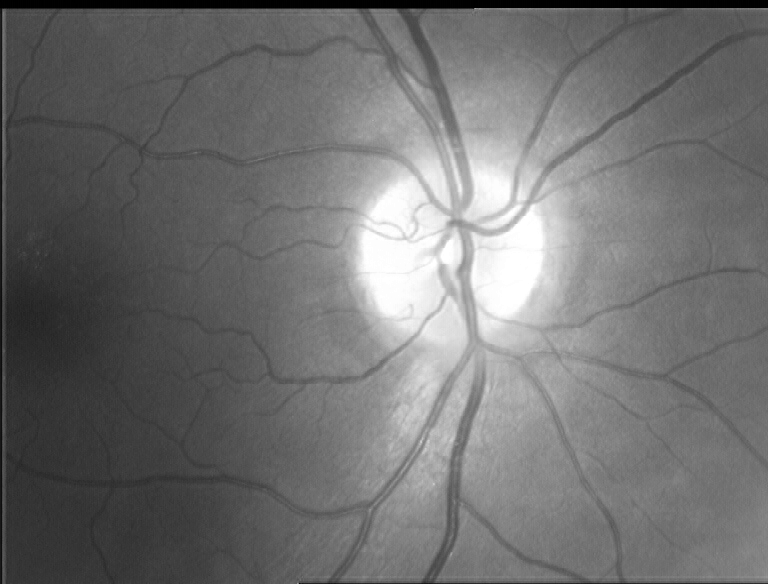
\includegraphics[width=6cm]{chap02/118}
        \centerline{(a)}\medskip
    \end{minipage}
  \begin{minipage}[b]{0.48\textwidth}
    \centering
    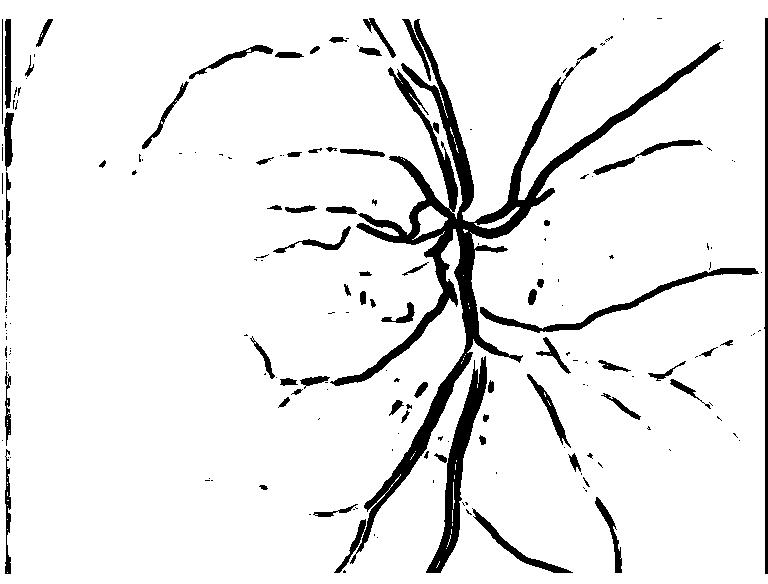
\includegraphics[width=6cm]{chap02/118-13}
      \centerline{(b)}\medskip
  \end{minipage}
  \begin{minipage}[b]{0.48\textwidth}
    \centering
    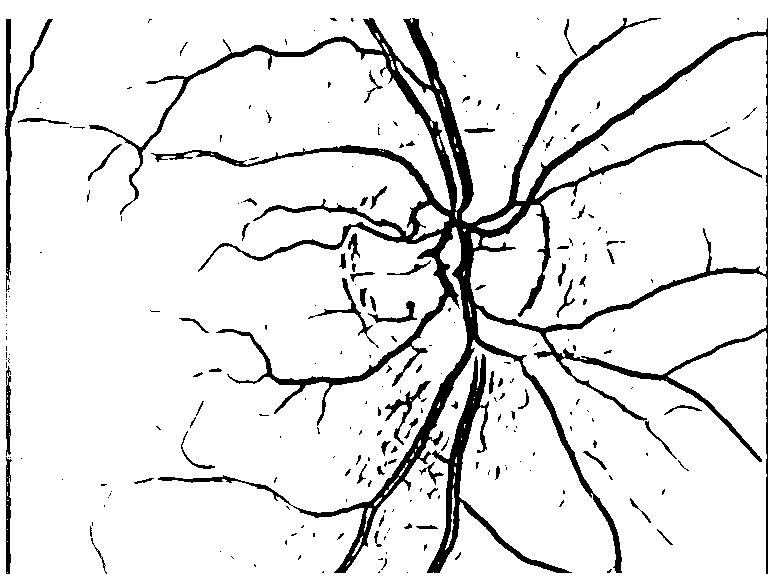
\includegraphics[width=6cm]{chap02/118-08}
      \centerline{(c)}\medskip
  \end{minipage}
  \begin{minipage}[b]{0.48\textwidth}
    \centering
    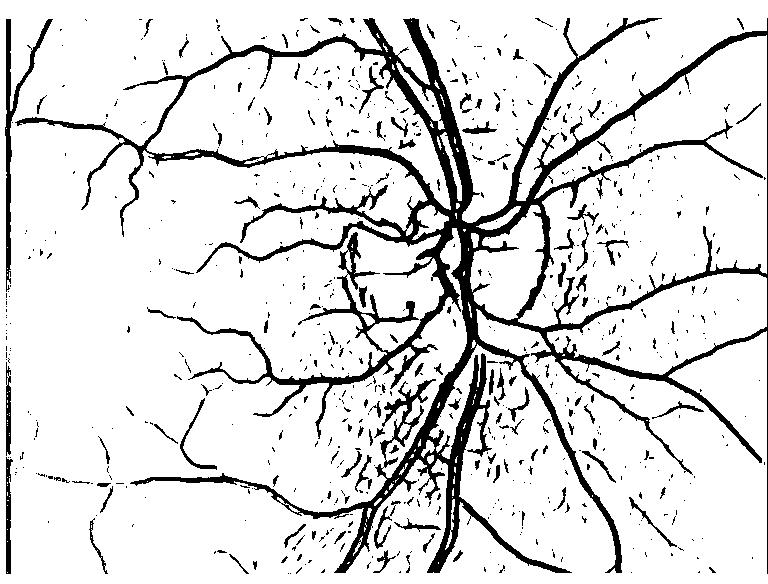
\includegraphics[width=6cm]{chap02/118-01}
      \centerline{(d)}\medskip
	\label{fig:max}
  \end{minipage}
\caption{不同尺度的视网膜图像分割结果。a为原图,b、c、d分别代表不同尺度的分割结果。}
\label{fig:Segmentaion-retinal}
\end{figure}

\begin{figure}
\centering
  \begin{minipage}[b]{0.48\textwidth} 
      \centering 
      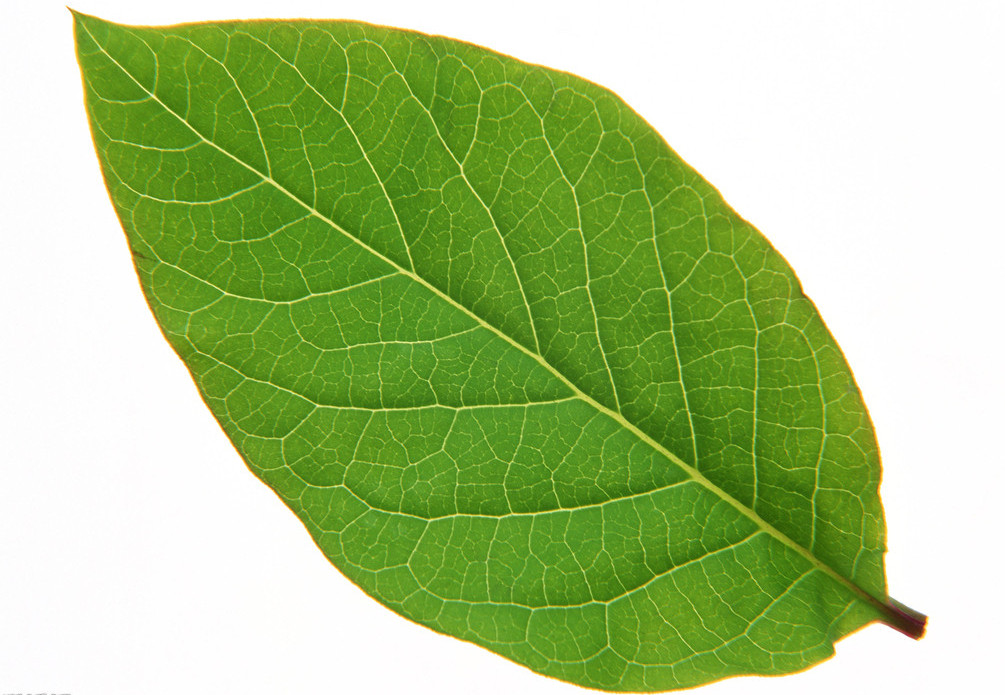
\includegraphics[width=6cm]{chap02/reaf-origin}
        \centerline{(a)}\medskip
    \end{minipage}
  \begin{minipage}[b]{0.48\textwidth}
    \centering
    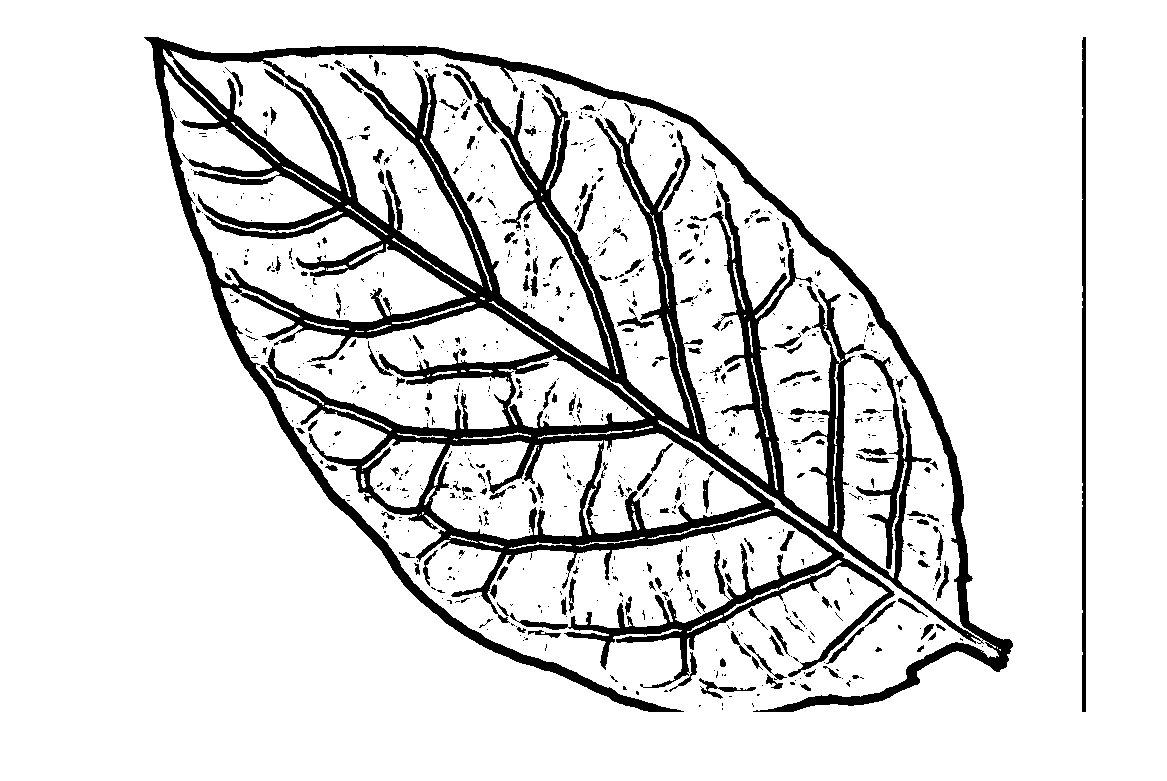
\includegraphics[width=6cm]{chap02/reaf1}
      \centerline{(b)}\medskip
  \end{minipage}
  \begin{minipage}[b]{0.48\textwidth}
    \centering
    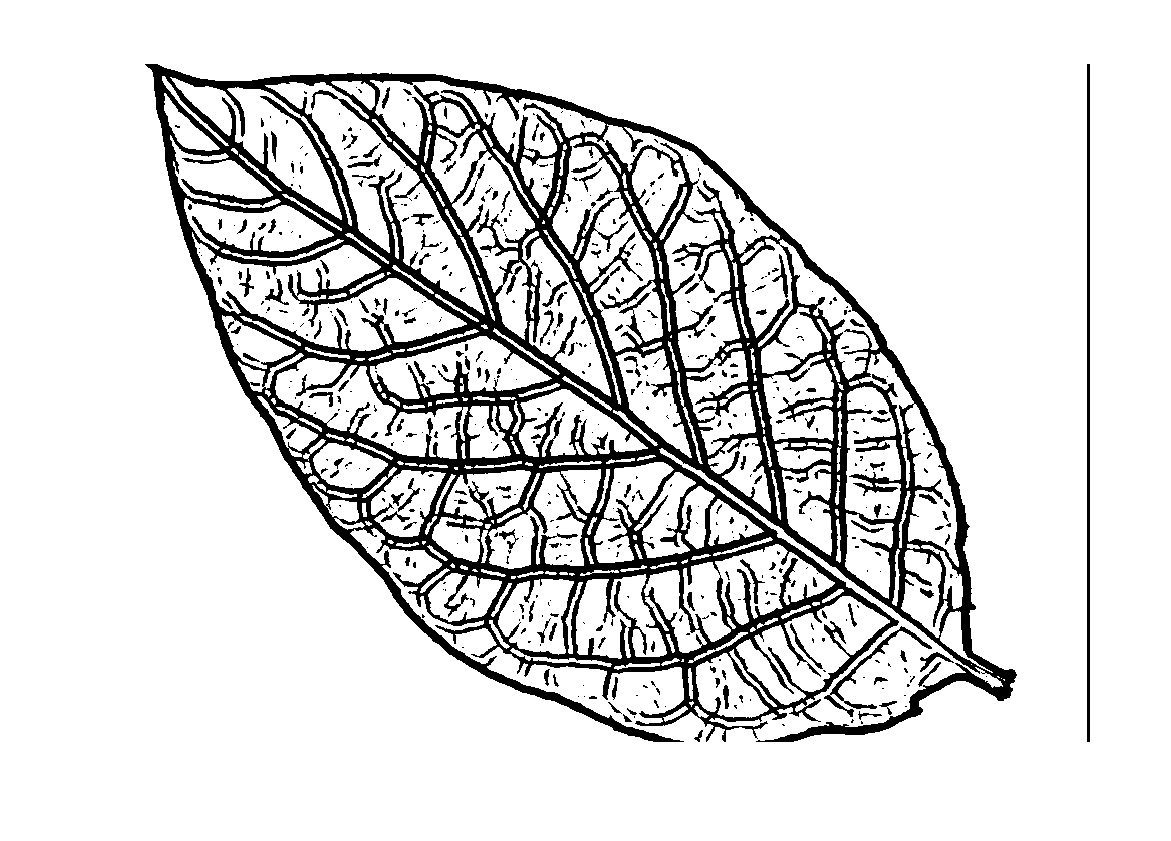
\includegraphics[width=6cm]{chap02/reaf3}
      \centerline{(c)}\medskip
  \end{minipage}
  \begin{minipage}[b]{0.48\textwidth}
    \centering
    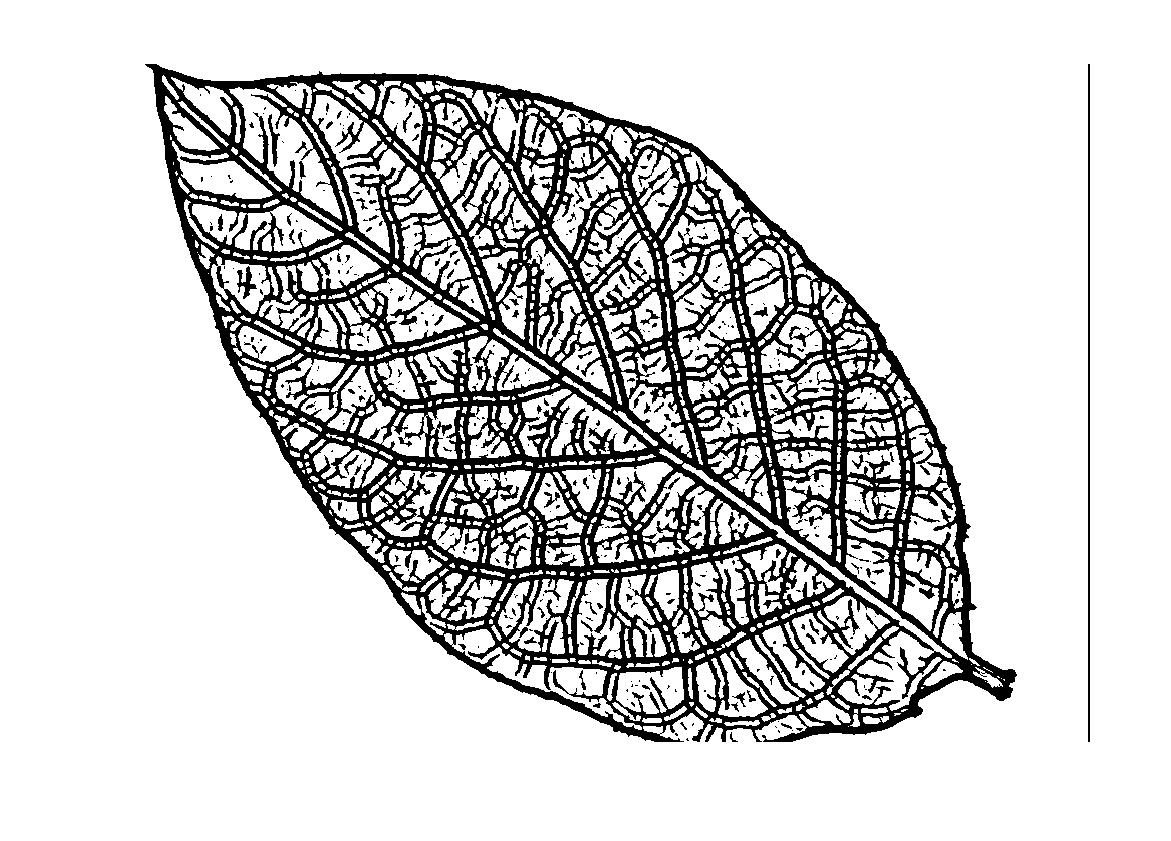
\includegraphics[width=6cm]{chap02/reaf2}
      \centerline{(d)}\medskip
	\label{fig:max}
  \end{minipage}
\caption{不同尺度的树叶图像分割结果。a为原图,b、c、d分别代表不同尺度的分割结果}
\label{fig:Segmentaion-retinal1}
\end{figure}

然而,若原图亮度不均或背景中存在较大噪声,分割尺度较大时虽然会把图像的细节分割出来,但噪声也会随之被分割出来,这样就增加环结构提取的困难度。为了消除噪声对环结构提取的影响,要对分割后的图像进行去噪处理。

\subsection{连通区域标记图像去噪}

连通区域标记\cite{xuzhengguang}是图像处理中常用的一个基本方法,在目标分割、边缘检测中有着十分广泛的应用。同时,连通区域也可应用于图像去噪。
采用连通区域算法对连通区域进行标记,即通过对二值图像进行逐行逐列扫描,根据图像中像素之间的邻域关系,对属于同一四连通或八连通区域的像素赋予相同的标号,然后统计同一标号的像素的个数。若像素数小于某个阈值,则认为是噪声。

邻域关系有两种,即四邻域与八邻域。设像素$P(x, y)$,则像素P的四邻域表示为$P_1(x,y-1), P_2(x, y+1), P_3(x-1,y), P_4(x+1,y)$,像素P的八邻域表示为$P_1(x,y-1), P_2(x, y+1), P_3(x-1,y), P_4(x+1,y), P_5(x-1,y-1), P_6(x+1, y+1), P_7(x-1,y+1), P_8(x+1, y-1)$,更加直观的表示如表\ref{tab:adjacent}。为了更好的去除噪声,我们采用八邻域去噪。
\begin{table}[H]
\centering
\caption{四邻域与八邻域}
\begin{tabular}{|c|c|c|}
\hline
 & $P_1$ & \\
\hline            
$P_3$ & $P$ & $P_4$\\
\hline           
& $P_2$ & \\
\hline
\end{tabular}
\begin{tabular}{|c|c|c|}
\hline
$P_5$ & $P_1$ & $P_7$\\
\hline            
$P_3$ & $P$ & $P_4$\\
\hline            
$P_8$& $P_2$ & $P_6$ \\
\hline
\end{tabular}

\label{tab:adjacent}
\end{table}


图\ref{fig:denoise-table}是一幅二值图像的连通区域标记图,从图中可以看出,共有2个连通区域,标号为1、2。其中连通区域1只有两个像素,连通区域2有11个像素,若设定10个像素为基准,小于10个像素的连通区域为噪声,则连通区域1将被认为是噪声,进行去除,而连通区域2将被保留。\ref{fig:Preprocessing}(b)是图\ref{fig:Preprocessing}(a)经过去噪后的结果,从图中可以看出很多的噪声都被滤除了。这一步骤不仅会减小环提取过程的复杂性,也避免了噪声形成的假环结构被提取出来的情况。


\begin{figure}[H] % use float package if you want it here
  \centering
  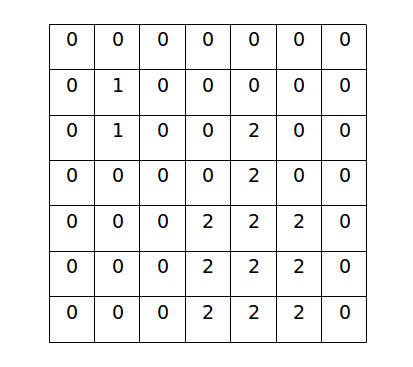
\includegraphics[width=0.4\textwidth]{chap02/denoise-table}
  \caption{连通区域标记去噪。区域1只有两个像素,若设置10个像素为阈值,则1被认为是噪声,需被去除。}
  \label{fig:denoise-table}
\end{figure}



\subsection{膨胀腐蚀操作填充孔洞}
在有些情况下,有时图像的亮度值不均匀,这就造成了分割出的线是断裂的或有孔洞的情况,为了骨架化后的图像能准确的体现原图像的特征,需对分割后的图像进行先膨胀后腐蚀操作。
膨胀腐蚀是图像形态学中比较常见的处理,一般是对二值图像进行处理。
用b对函数f进行的灰度膨胀\cite{gang}表示为:
\begin{align}
(f\oplus b)(s,t)=max\{f(s-x, t-y)+b(x,y)|(s-x),(t-y)\in D_f;(x,y)\in D_b\}
\end{align}
其中,$D_f$和$D_b$分别是f和b的定义域。
灰度腐蚀表示为$f \ominus b$,定义为:
\begin{align}
(f \ominus b)(s,t)=min\{f(s+x, t+y)-b(x,y)|(s+x),(t+y)\in D_f;(x,y)\in D_b\}
\end{align}

图\ref{fig:peng-fu}显示了先膨胀后腐蚀与先腐蚀后膨胀的区别。a、d为原图,三个黑色矩形块之间的两个空隙分别为5个与10个像素,若采用$5\times5$的矩形窗口对图像进行膨胀腐蚀与腐蚀膨胀操作,得到的最终结果如图c与e。从图中可以看到,先膨胀后腐蚀后,狭窄的缝隙被填充了,而在此例中先腐蚀后膨胀后得到的结果与原图相同。视网膜图像的示例如图\ref{fig:Preprocessing}(c)所示,血管中心位置的孔洞被成功填充。

\begin{figure}
\centering
  \begin{minipage}[b]{0.3\textwidth} 
      \centering 
      
\includegraphics[width=6cm]{chap02/peng-origin}
        \centerline{(a)原图}\medskip
    \end{minipage}
  \begin{minipage}[b]{0.3\textwidth}
    \centering
    
\includegraphics[width=6cm]{chap02/peng-fu}
      \centerline{(b)膨胀}\medskip
  \end{minipage}
  \begin{minipage}[b]{0.3\textwidth}
    \centering
    
\includegraphics[width=6cm]{chap02/peng-fu}
      \centerline{(c)膨胀后腐蚀}\medskip
  \end{minipage}
   \begin{minipage}[b]{0.3\textwidth} 
      \centering 
      
\includegraphics[width=6cm]{chap02/peng-origin}
        \centerline{(d)原图}\medskip
    \end{minipage}
  \begin{minipage}[b]{0.3\textwidth}
    \centering
    
\includegraphics[width=6cm]{chap02/fu-peng1}
      \centerline{(e)腐蚀}\medskip
  \end{minipage}
  \begin{minipage}[b]{0.3\textwidth}
    \centering
    
\includegraphics[width=6cm]{chap02/fu-peng2}
      \centerline{(f)腐蚀后膨胀}\medskip
  \end{minipage}
\caption{先膨胀后腐蚀与先腐蚀后膨胀}
\label{fig:peng-fu}
\end{figure}

\subsection{骨架化}
为了获得一个像素宽的骨架化结果,我们采用轮廓修剪骨架提取方法~\footnote{http://www.cs.smith.edu/$\sim$nhowe/research/code/}。这个方法是Nicholas R. Howe实现的,想法是Alex Telea提出的。若一个点位于一个圆圈的中心,并接触一个图像边缘的多个点,灰度骨架化图像的强度是基于围绕图像的周长连接最远的两点的最短距离。因此,骨架中的毛刺是由微小的边缘扰动引起的强度变化。如果圆圈接触断裂的边缘,骨架化将会是无限的过程。最终的骨架化结果是通过噪声突起轮廓的预期大小来确定的阈值来决定的。图\ref{fig:Preprocessing}(d)是骨架化结果,从图中可以看到,骨架后的图像能准确的描绘出血管的主轮廓。
\begin{figure}[H]
\centering
  \begin{minipage}[b]{0.48\textwidth}
    \centering
    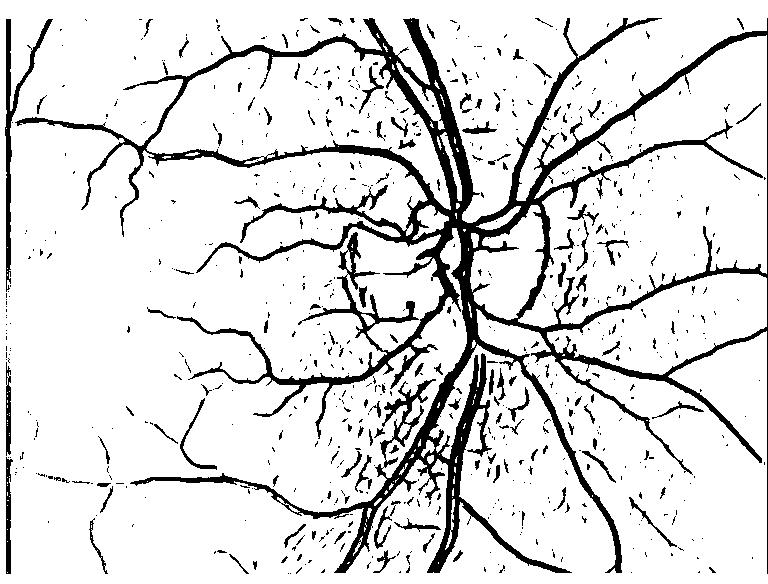
\includegraphics[width=6cm]{chap02/118-01}
      \centerline{(a) 分割图}\medskip
  \end{minipage}
  \begin{minipage}[b]{0.48\textwidth}
    \centering
    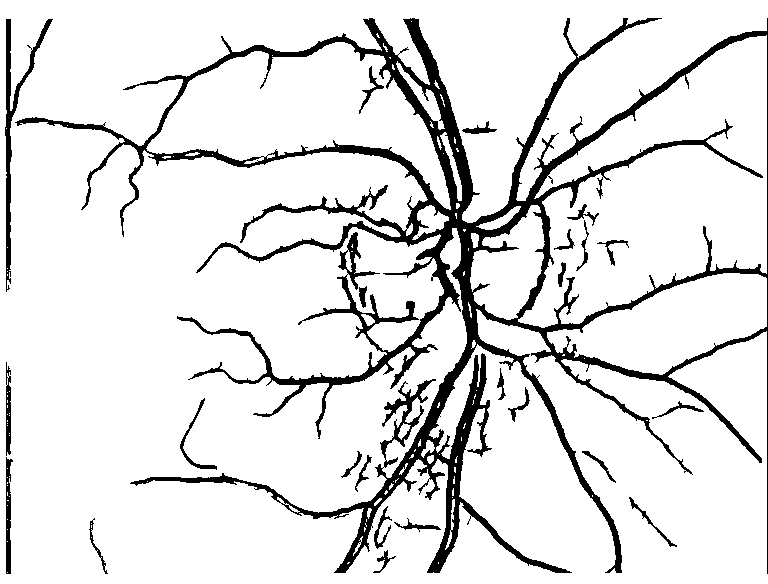
\includegraphics[width=6cm]{chap02/denoise}
      \centerline{(b) 去噪图}\medskip
  \end{minipage}
  \begin{minipage}[b]{0.48\textwidth}
    \centering
    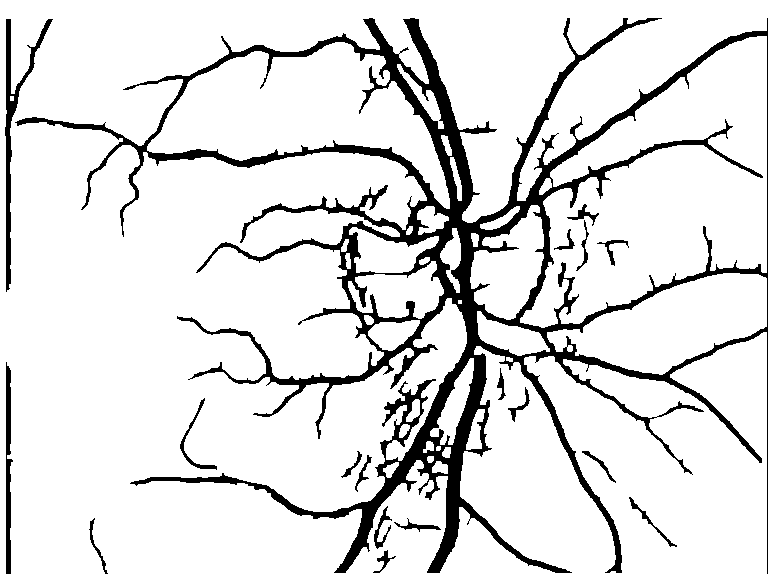
\includegraphics[width=6cm]{chap02/fill}
      \centerline{(c) 填充图}\medskip
  \end{minipage}
  \begin{minipage}[b]{0.48\textwidth}
    \centering
    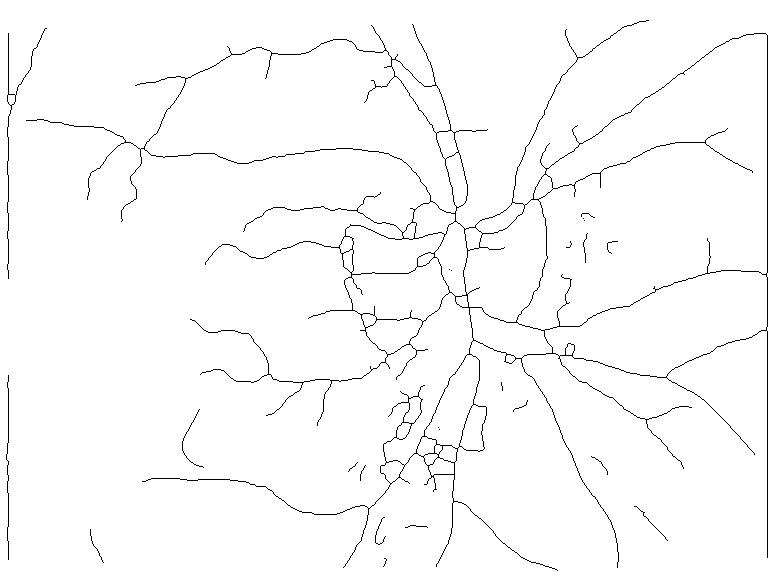
\includegraphics[width=6cm]{chap02/118-skel}
      \centerline{(d) 骨架图}\medskip
  \end{minipage}
\caption{预处理}
\label{fig:Preprocessing}
\end{figure}

经过这四个步骤,各类彩色图像就变为去噪后的骨架化二值图像,其中的环结构具有一个像素宽度,这样就为检测环结构做好了准备。

\section{环结构检测}
\label{}
\subsection{图论相关概念}
\label{}

图像中环的概念是由图论扩展而来的。在人类社会的实际生活中,有时在描述某些事物或对象之间有某种特定关系时采用图形的方式显得更加直观。对象用图形中的点表示,两对象之间具有的某种特定的关系用两点之间的无向或有向连线表示,由此数学抽象产成了图的概念。

\begin{definition}
一个图$G$定义为一个数学结构$(V, E, \phi)$\cite{xujunming},其中
\begin{enumerate}
\item $V$是一个集合,其中的元素成为顶点;
\item $E$是定义在$V$上的可以重复的二元关系集,其中的元素成为边;
\item $\phi$ 是$E$到$V$的一个映射。 
\end{enumerate}
若$\phi(E)$中的元素全是有序对,则$(V, E, \phi)$成为有向图,否则,成为无向图。我们所研究的图像中的线是无方向的,所以我们可以把图像认为是无向图。
\end{definition}

在图像中,顶点可以定义为线的交叉、分叉点或孤立点,边为连接两个顶点的连线,如图\ref{fig:graph}所示,$V = \{v_1, v_2, v_3, v_4, v_5\}$,$E = \{e_1, e_2, e_3, e_4\}$,边$e_1$把顶点$v_1, v_2$连接起来。

\begin{figure}[H] % use float package if you want it here
  \centering
  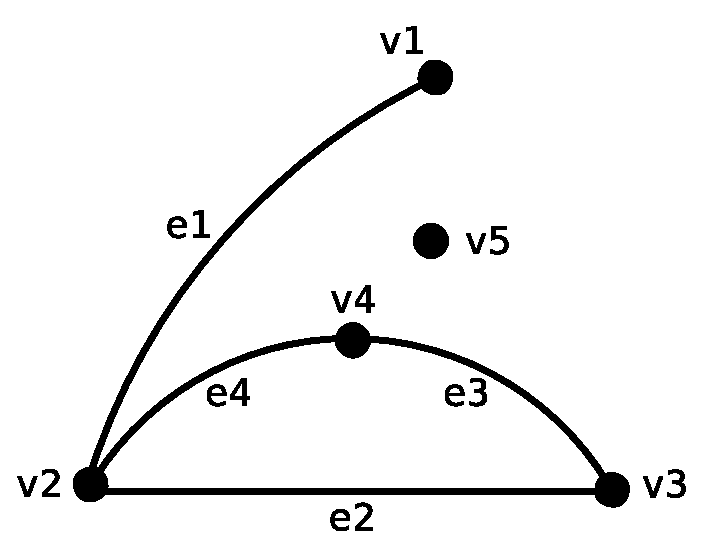
\includegraphics[width=0.3\textwidth]{chap02/graph}
  \caption{图}
  \label{fig:graph}
\end{figure}

\begin{definition}
设$G$是无向图,$x\in V(G)$的顶点度定义为$G$中与$x$关联边的数目,记为$d_{G}(x)$\cite{wangshuhe}。
\end{definition}

图\ref{fig:graph}中,只有一条边$e_1$与顶点$v_1$相连,即$d_{v_1}=1$,类似的,$d_{v_2}=3, d_{v_5}=0$。


\begin{definition}
设无向图$G = (V, E), v_i, v_j \in V$,若存在一条边$e$以$v_i, v_j$为端点,即$e = (v_i, v_j)$,则称$v_i, v_j$是彼此相邻的,简称相邻的。 
\end{definition}
例如,图\ref{fig:graph}中,$v_1$与$v_2$是相邻的,$v_2$与$v_5$是不相邻的。

设$(V, E, \phi)$是无向图$G$,其中$V = \{v_1, v_2, \ldots, v_p\}$,$E = \{e_1, e_2, \ldots, e_\varepsilon\}$。则无向图G的邻接矩阵能够反映出V中元素与E中元素之间的关联关系。
\begin{definition}
设图G的顶点集$V = \{v_1, v_2, \ldots, v_p\}$,令
\begin{align}
a_{ij} = \left\{ \begin{array}{ll}
1 & \textrm{$v_i$与$v_j$相邻}\\
0 & \textrm{$v_i$与$v_j$不相邻或$i = j$}
\end{array} \right.
\end{align}
则称由元素$a_{ij} (i, j == 1, 2, \ldots, p)$构成的p阶矩阵为图G的邻接矩阵\cite{wangzhaorui},记作A。
\end{definition}
图\ref{fig:graph}的邻接矩阵是
\begin{align}
A = \left( \begin{array}{lllll}
0 & 1 & 0 & 0 & 0 \\
1 & 0 & 1 & 1 & 0 \\
0 & 1 & 0 & 1 & 0 \\
0 & 1 & 1 & 0 & 0 \\
0 & 0 & 0 & 0 & 0 
\end{array} \right)
\end{align}

无向图中的环是指一系列边的集合,起始点与终止点是重合的。一些环的集合成为一个环基。在无向无权图中,环的权重为组成这个环的边的数量。最小环基就表示能使组成这个环基的权重的总和最小的环的集合。图\ref{fig:graph}中,共存在九个环,即:$c_1 = < v_1, v_2, v_3>, c_2 = <v_4, v_5, v_6>, c_3 = <v_5, v_6, v_7, v_8, v_{10}>, c_4 = <v_8, v_9, v_{10}>, c_5 = < c_{14}, c_{15}, c_{16}>, c_6 = <v_{10}, v_{11}, v_{12}, v_{13}>, c_7 = <c_4, c_5, v_{10}, v_9, v_8, v_7, v_6>, c_8 = < v_6, v_5, v_{10}, v_9, v_8, v_7>, v_9 = < v_4, v_5, v_{10}, v_9, v_8, v_7, v_6>$,其中,$c_1, c_2, c_3, c_4, c_5$是最小环,他们组成的集合为最小环基,即$M = \{c_1, c_2, c_3, c_4, c_5\}$。
\begin{figure}[H]
\centering
    \centering
    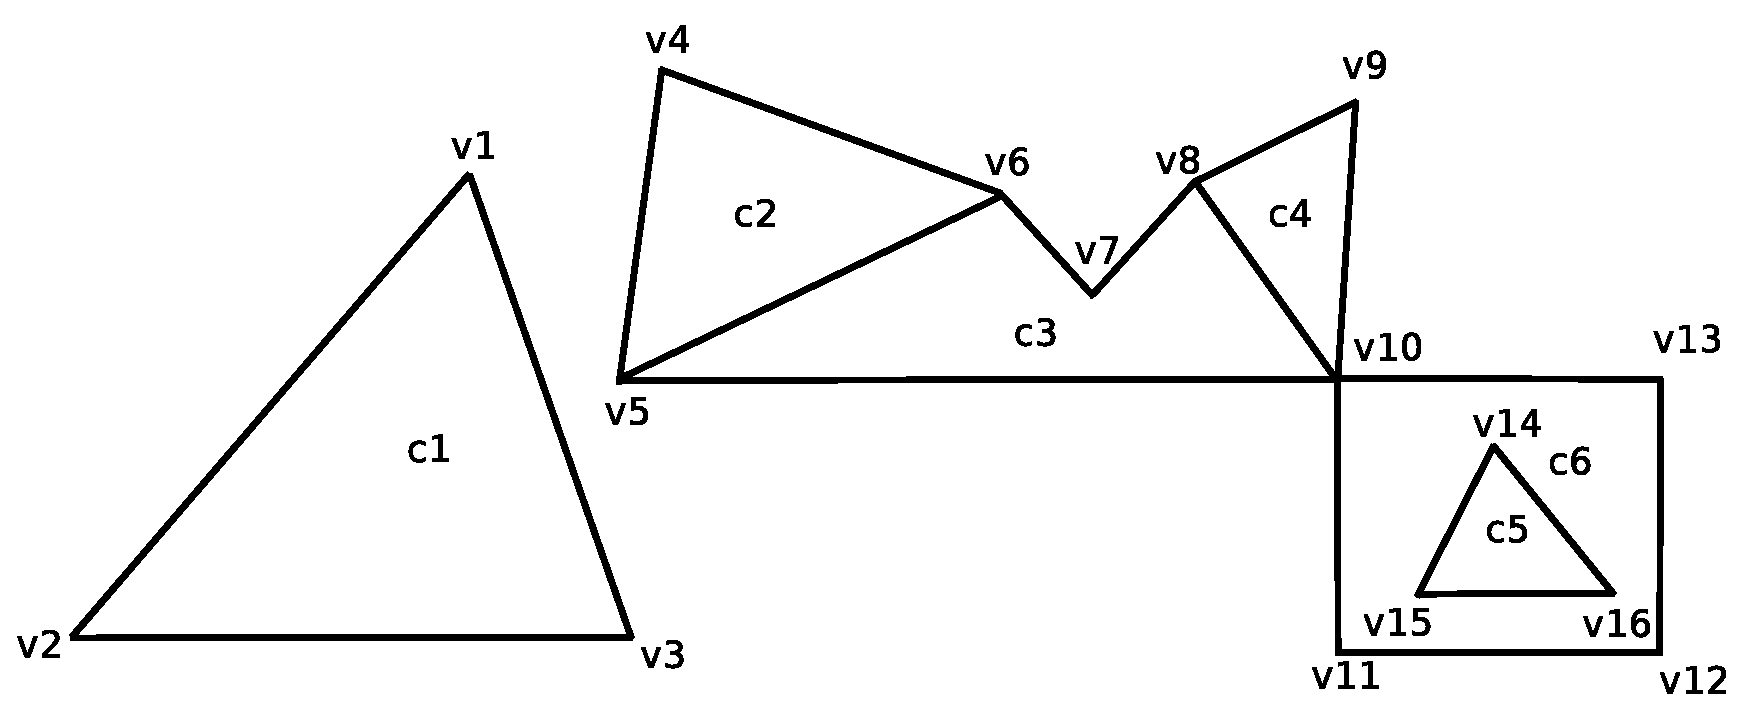
\includegraphics[width=10cm]{chap02/graph-cycle}\medskip
\caption{图中的环}
\label{fig:graph-cycle}
\end{figure}


检测图中的所有的环的问题,实际上就是检测图中的最小环基的问题。要在图像中检测最小环基,首先应先检测分叉点及其之间的连接关系,根据其连接关系,构造搜索路径,以此来实现检测环的过程。

\subsection{分叉点与连接关系检测}
\label{}

二值图像中,若背景为黑,即其像素值是0,线为白,即像素值是1。要判断一个像素点是否为分叉点,首先应定位线的位置,即判断像素值是否为1,然后判断这个像素点的八邻域像素为1的像素个数,若八邻域没有像素为1的像素,则认为是度为1的顶点,即孤立点,若八邻域有1个像素值为1的像素,则认为这两个点形成一条短线段,这些点都不认为是分叉点。这样研究对象为八邻域内有大于等于3个像素值为1的点。通过观察与实验发现若八邻域有3个像素值为1的像素,则中心点其八邻域像素值为1的点形成三分叉,中心点可被认为是三分叉点,如图\ref{fig:FeaturePoints}所示,图(a)中的红色点八邻域内有3个值为1的点,则红色点为三分叉点。三分叉点的常见情况如图\ref{fig:FeaturePoints-image}(a)所示。

而若某一点的八邻域有三个以上像素值为1的像素,则不能单纯的认为是几分叉点,如图\ref{fig:FeaturePoints}(b)所示是四分叉点的例子,红色点及蓝色点八邻域都有3个以上的值为1的点,但蓝色点不能认为是分叉点。

这种情况下,我们要进行连通区域标记。首先重新定位可能是分叉点的点,即其八邻域有3个以上像素值为1的点。然后要进行连通区域标记,图\ref{fig:FeaturePoints}(b)中的红色及蓝色点标记为一个区域,根据标记点的坐标,计算连通区域的中心位置,最后把中心位置点作为同一个连通区域的分叉点,而连通区域内的其他点为普通点,即红色点作为连通区域的中心,看作是真正的四分叉点。在图像中\ref{fig:FeaturePoints}(b)显示为\ref{fig:FeaturePoints-image}(b),通过计算,蓝色点为中心位置点,即四分叉点。

\begin{figure}
\centering
  \begin{minipage}[b]{0.48\textwidth} 
      \centering 
      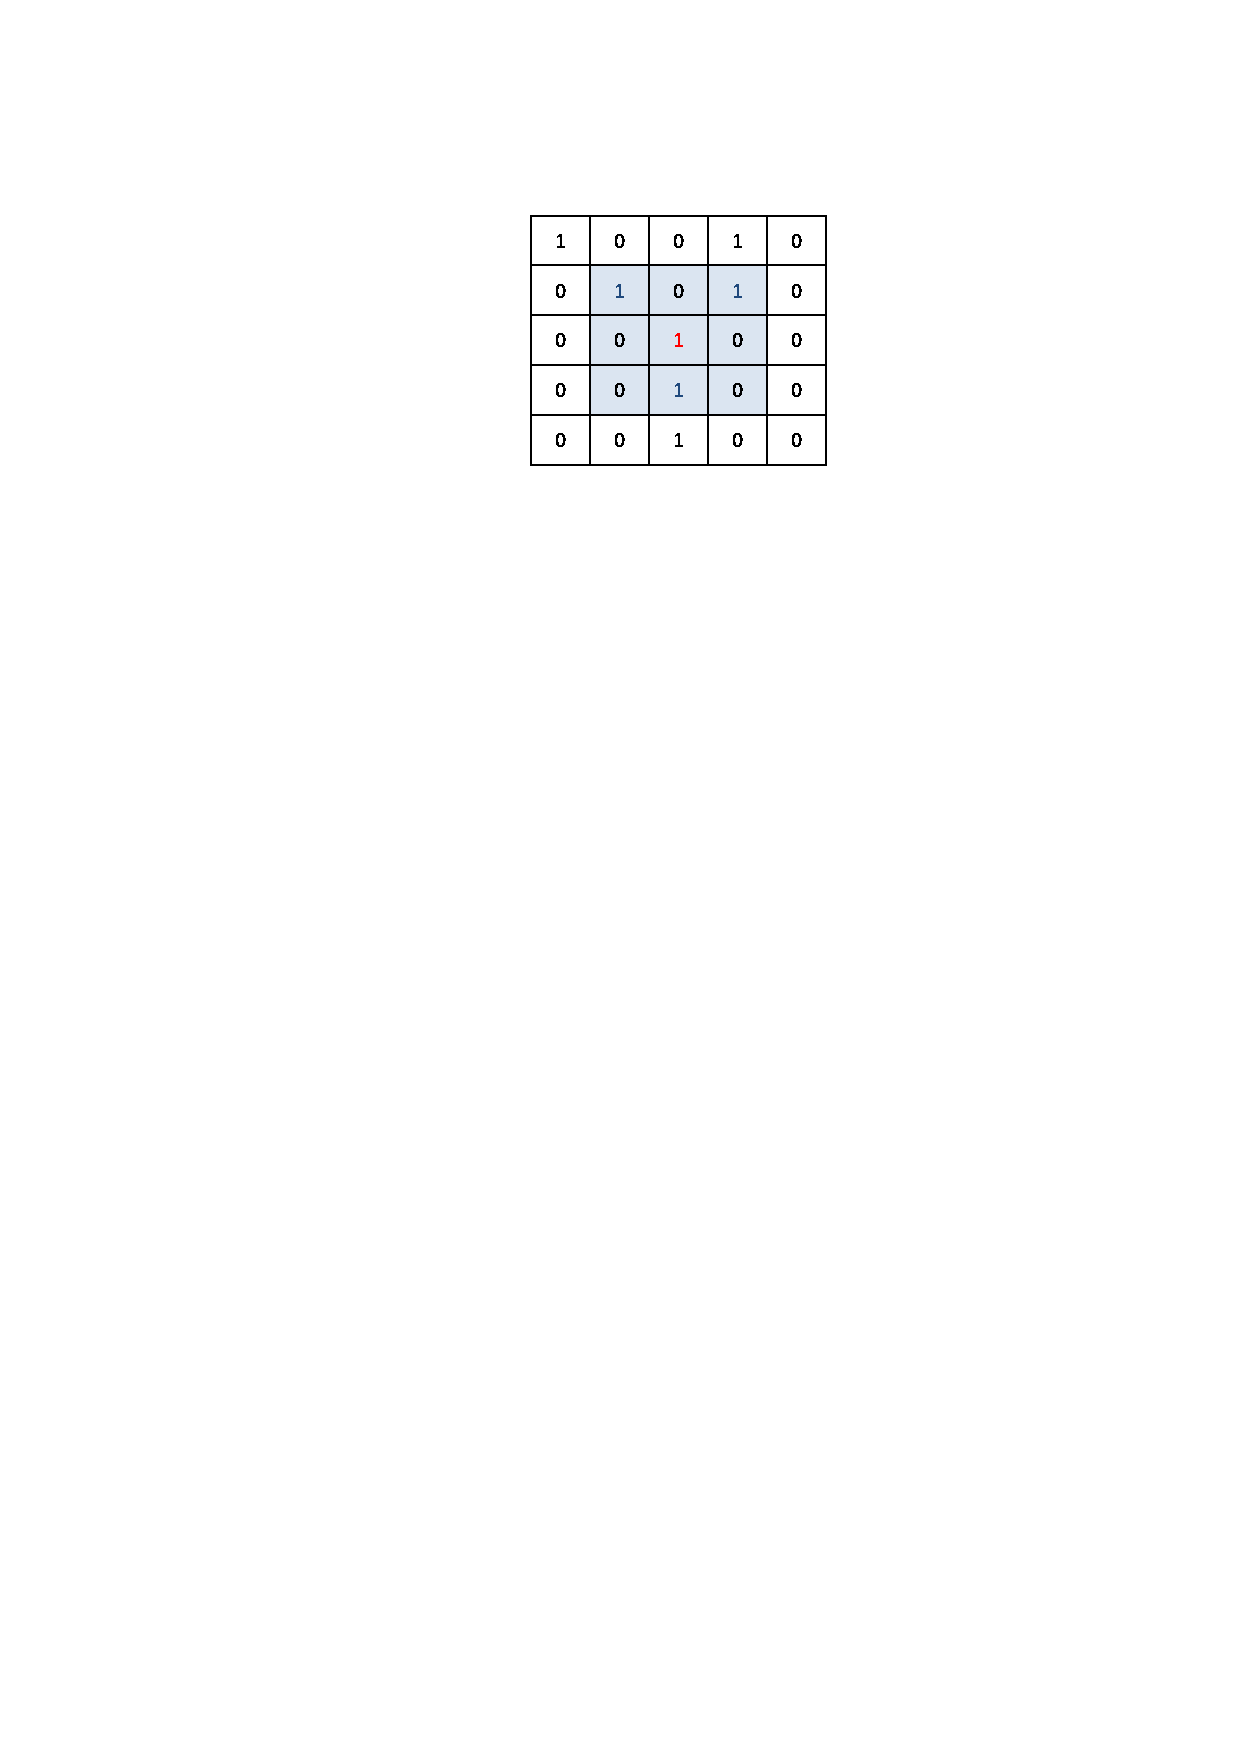
\includegraphics[width=4cm]{chap02/3FeaturePoint}
        \centerline{(a)}\medskip
	 \label{fig:3FeaturePoint}
    \end{minipage}
  \begin{minipage}[b]{0.48\textwidth}
    \centering
    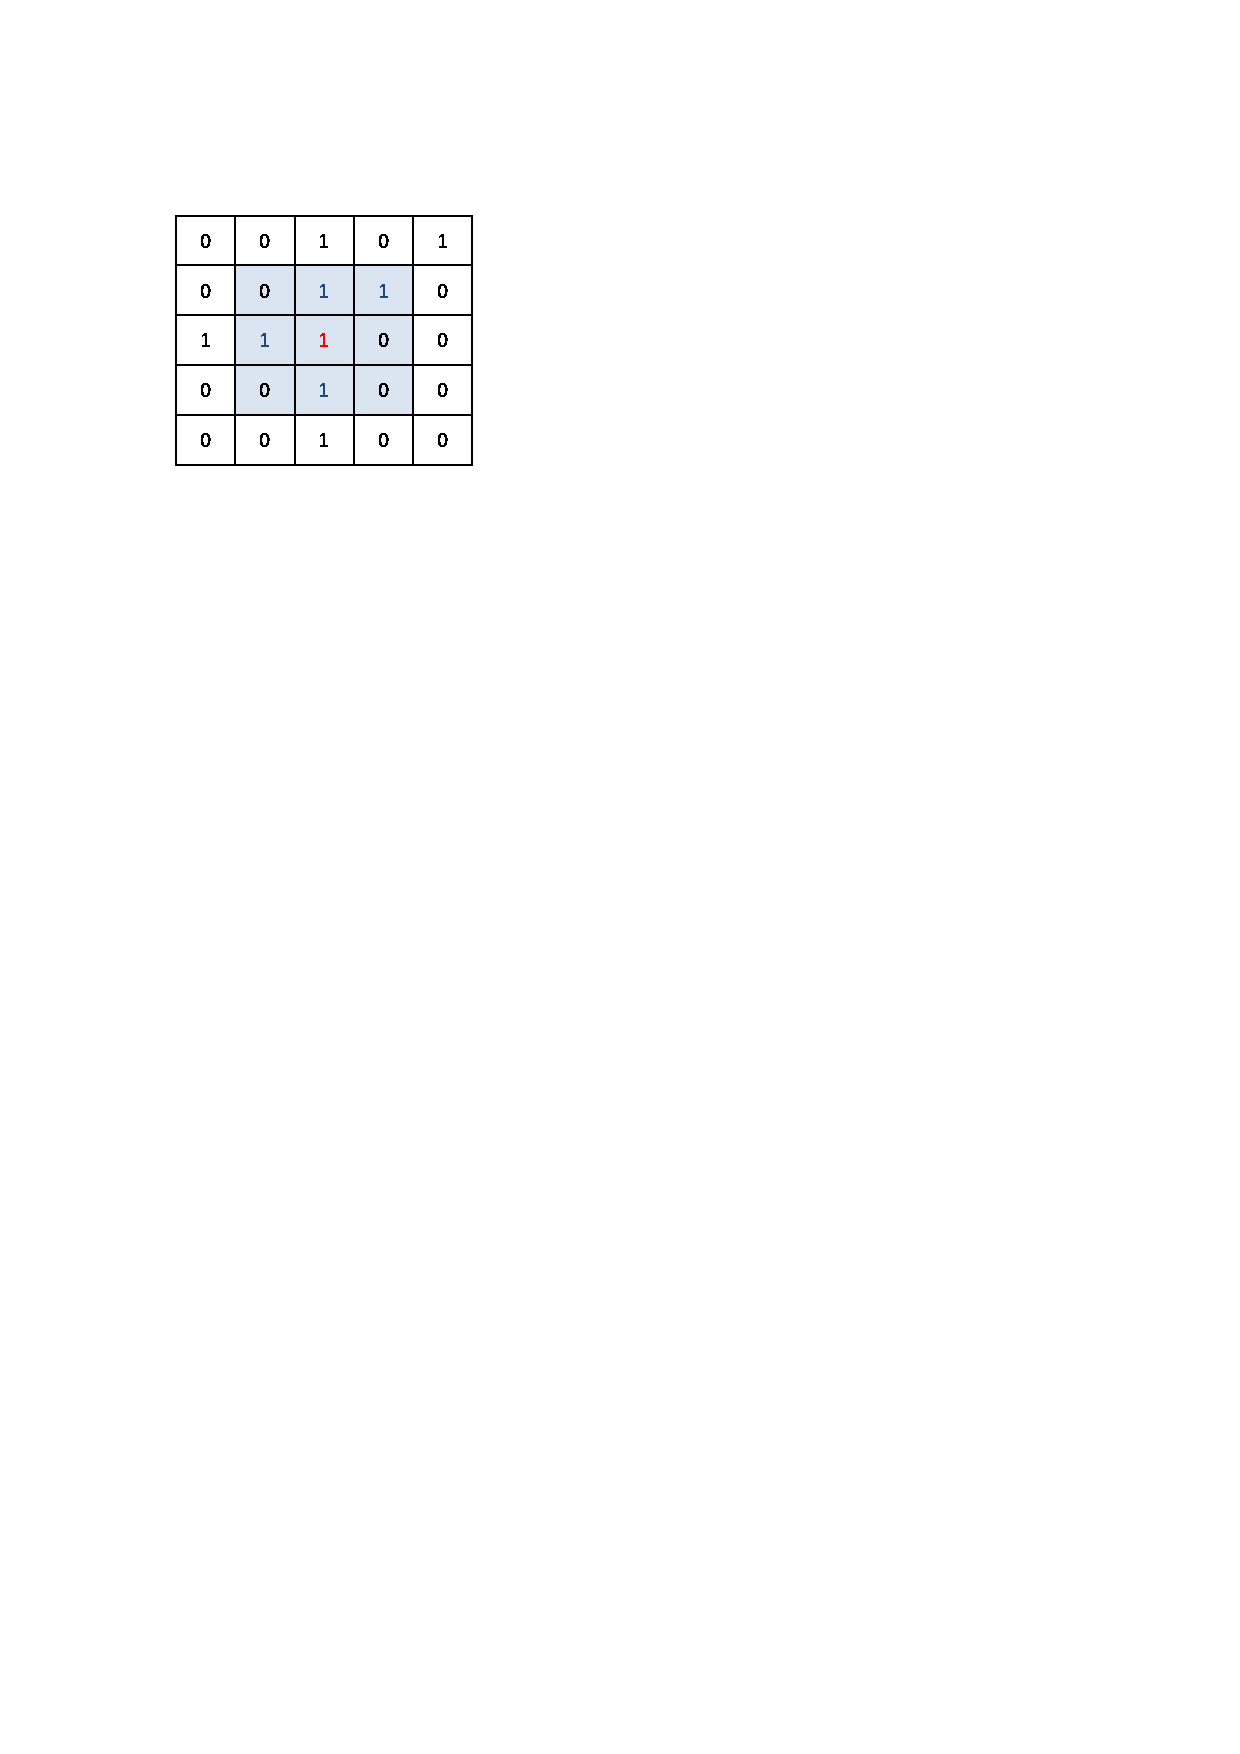
\includegraphics[width=4cm]{chap02/4FeaturePoint}
      \centerline{(b)}\medskip
	\label{fig:4FeaturePoint}
  \end{minipage}
\caption{三分叉点与四分叉点}
\label{fig:FeaturePoints}
\end{figure}

\begin{figure}
\centering
  \begin{minipage}[b]{1\textwidth} 
      \centering 
      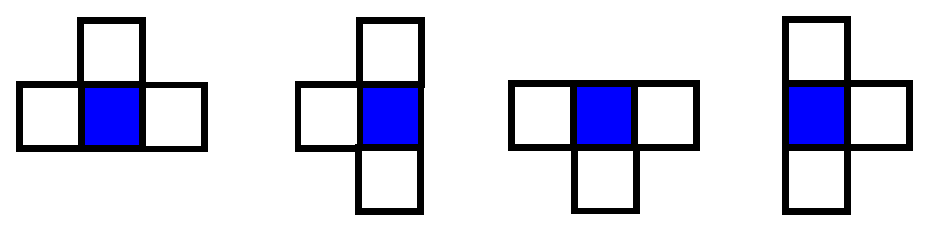
\includegraphics[width=8cm]{chap02/three-bifu}
        \centerline{(a)}\medskip
    \end{minipage}
  \begin{minipage}[b]{1\textwidth}
    \centering
    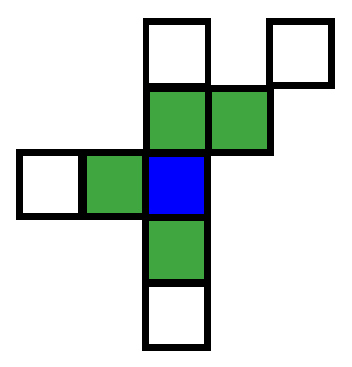
\includegraphics[width=3cm]{chap02/four-bifu}
      \centerline{(b)}\medskip
  \end{minipage}
\caption{三分叉点与四分叉点}
\label{fig:FeaturePoints-image}
\end{figure}

当所有的分叉点都检测到后,每个分叉点被看做一个种子,沿其八邻域像素值为1的方向不断向外扩展,直到找到与这个分叉点相邻的分叉点。遍历所有分叉点后,所有的分叉点及其连接关系就被检测到。为了方便后续操作,我们将采用顶点---边矩阵来表示分叉点及其连接关系,于是得到图\ref{fig:graph}的点---边关系表\ref{tab:AdjacentStructure},第一列为所有的分叉点,其余几列为与分叉点相连的分叉点。
\renewcommand\arraystretch{0.8}
\begin{table}[H]
\caption{点---边关系}
\centering
\begin{tabular}{p{2cm}<{\centering}p{1cm}<{\centering}p{1cm}<{\centering}p{1cm}<{\centering}}
  \hline
  分叉点 & \multicolumn{3}{c}{相邻分叉点}\\
  \hline
  \rowcolor{gray!50}
  $v_{1}$ & $v_{2}$  & $0$      & $0$  \\
  $v_{2}$ & $v_{1}$  & $v_{3}$  & $v_{4}$ \\
  \rowcolor{gray!50}
  $v_{3}$ & $v_{2}$  & $v_{4}$  & $0$\\
  $v_{4}$ & $v_{2}$  & $v_{3}$  & $0$ \\
  \rowcolor{gray!50}
  $v_{5}$ & $0$      & $0$      & $0$\\
  \hline
\end{tabular}
\label{tab:AdjacentStructure}
\end{table}

众所周知,能够组成环结构的分叉点数目至少为3,这就要求每个分叉点的度大于等于3,即$d_{v_i} \geq 3$,并且每个分叉点应至少在点---边关系矩阵中出现3次。通过这个规则,可以滤除一些不能组成环结构的点。但这个过程不能一次滤除所有的不能组成环结构的无效点,而是需要进行循环滤除,每进行一次,最外围的无效点将会滤除,直到所有的无效点被滤除后,循环得以结束。以一个视网膜图像为例,如图\ref{fig:Bifurcation},分别表示初始检测到的分叉点与所有无效分叉点被滤除后的图像,从图中可以看出,分支末端的点都被滤除,只剩下可能组成环的分叉点。通过滤除不能组成环的无效的分叉点,就可以大大的减少搜索环的路径,从而减小环检索算法的复杂度。

\begin{figure}
\centering
  \begin{minipage}[b]{0.48\textwidth} 
      \centering 
      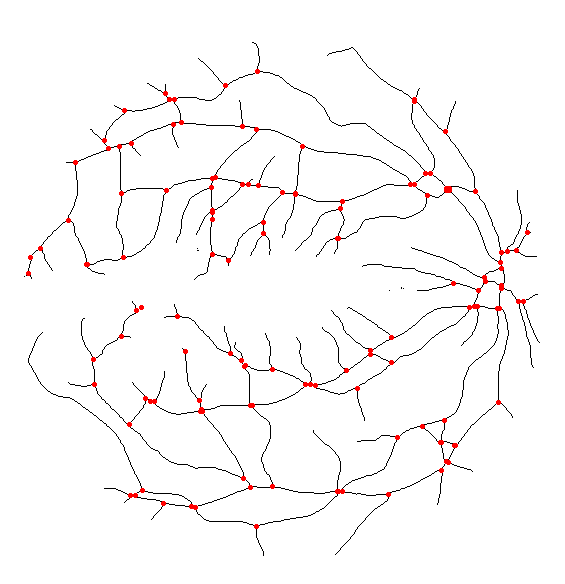
\includegraphics[width=4cm]{chap02/all-bifu}
        \centerline{(a)所有分叉点}\medskip
	 \label{fig:3FeaturePoint}
    \end{minipage}
  \begin{minipage}[b]{0.48\textwidth}
    \centering
    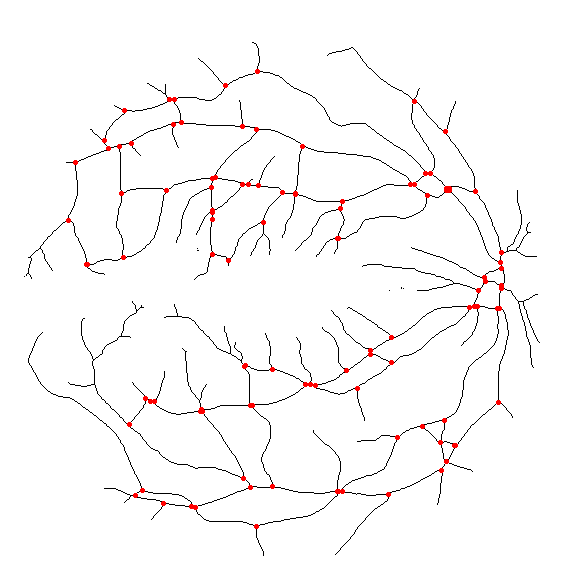
\includegraphics[width=4cm]{chap02/select-bifu}
      \centerline{(b) 可能组成环的分叉点}\medskip
	\label{fig:4FeaturePoint}
  \end{minipage}
\caption{所有分叉点与滤除无效分叉点后的对比图}
\label{fig:Bifurcation}
\end{figure}

\subsection{基于广度优先策略的环结构检测}
\label{}


在图中检测最小环基的问题实际上是图论中的一个被广泛研究的问题。Joe Kirk 提出了迭代环计数算法,算法的基本思想是通过动态路径搜索环,动态路径实际上是把图变换成一棵树,路径表示树上的一个结点到另一个结点的连线,当一个节点在一条路径上出现两次,则表示这条路径上的点形成一个环。

树的定义如下:
树是包括n个结点的有限集合$T(n \geq 1)$\cite{zhangming},使得
\begin{enumerate}
\item 有且只有一个特定的成为根的结点。
\item 除根以外的其他结点被分成m个$(m \geq 0)$个不相交的有限集合$T_1, T_2, \ldots, T_m$,而每一个集合又都是树。其中,树$T_1, T_2, \ldots, T_m$称作这个根的子树。
\end{enumerate}

这个定义是递归的,即在树的定义中又用到了树的概念。在一棵树中,若存在节点k指点个结点$k'$的连线,则称k是$k'$的父结点,而$k'$是k的子结点,有向连线$<k, k'>$称作边。同一个父结点的子结点之间称为兄弟。树中没有父结点的结点称为根,没有子结点的结点称为树叶。若树中存在结点序列$k_0,k_1,\ldots,k_s$,使得$<k_0,k_1>,<k_1,k_2>,\ldots,<k_{s-1},k_s>$都是树中的边,则称从结点$k_0$到结点$k_s$存在一条路径。若有一条由k到达$k_s$的路径,则称k是$k_s$的祖先,$k_s$是k的子孙。图\ref{fig:tree}表示一棵树,A表示根结点,B、C是A的子结点,A是BC的父结点,BC为兄弟结点。ABDI是一条路径,其中A是I的祖先,I为A的子孙。

\begin{figure}
\centering
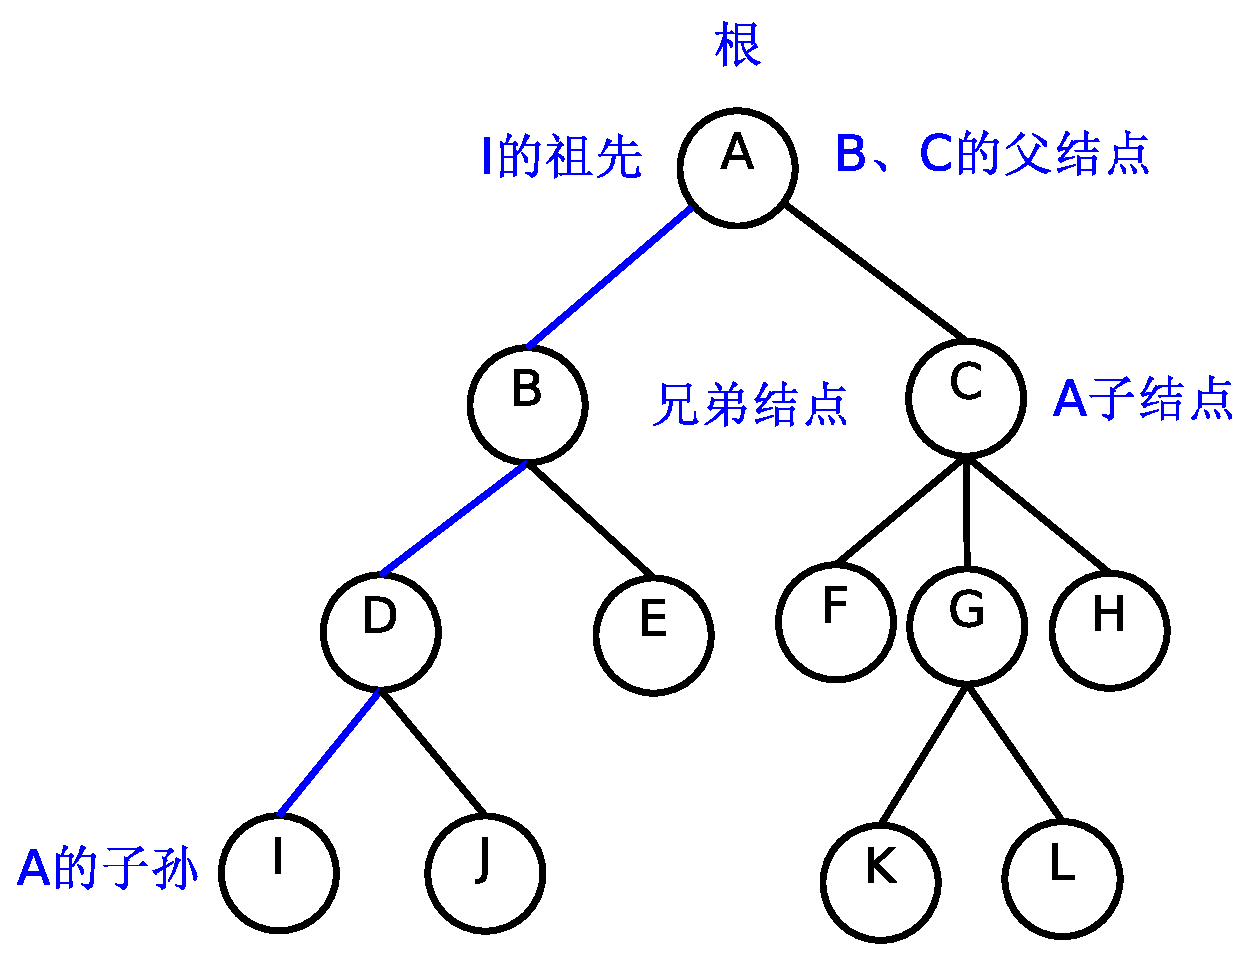
\includegraphics[width=0.5\textwidth]{chap02/tree-1}
\caption{树形表示法}
\label{fig:tree}
\end{figure}

在树中顺序搜索结点叫做树的遍历。通常有两种遍历方法:深度优先遍历与广度优先遍历。
\begin{itemize}

\item 深度优先遍历算法。深度优先算法的思想是尽可能沿分支结点向深度方向进行遍历。对于二叉树来说,深度优先即先沿着分支结点向左下降,当遇到左子树为空的时候,返回到上面最近的且其右子树尚未访问到的分支结点,转向该分支节点的右子结点,然后再尽可能地沿着左链前进。重复执行上述过程,直到遍历完所有的结点为止。

进行深度优先遍历时,结点既可以在向下遍历之前访问,也可以在从子树返回之后访问,根据结点的访问时间,可以定义不同的深度优先遍历算法,即前序法、中序法、后序法。前序法即先访问根结点,然后访问左子树,最后访问右子树。中序法先访问左子树,然后访问根结点,最后访问右子树。而后序法首先访问左子树,然后访问右子树,最后访问根结点。如图\ref{fig:dfs}所示为一个图,按前序法进行深度优先遍历时,访问结点的顺序应该是ABDECFG。

\item 广度优先遍历算法。广度优先又叫宽度优先或横向优先,是从上而下,从左到右地按层次进行遍历。其过程是:首先访问树的第一层,即根结点所在的层,然后从左到右依次访问第二层的结点,依次类推,当第i层的所有结点访问结束后,再从左到右依次访问第i+1层的各个结点。图\ref{fig:dfs}进行广度优先搜索的结果为ABCDEFG。

\end{itemize}

\begin{figure}[H]
\centering
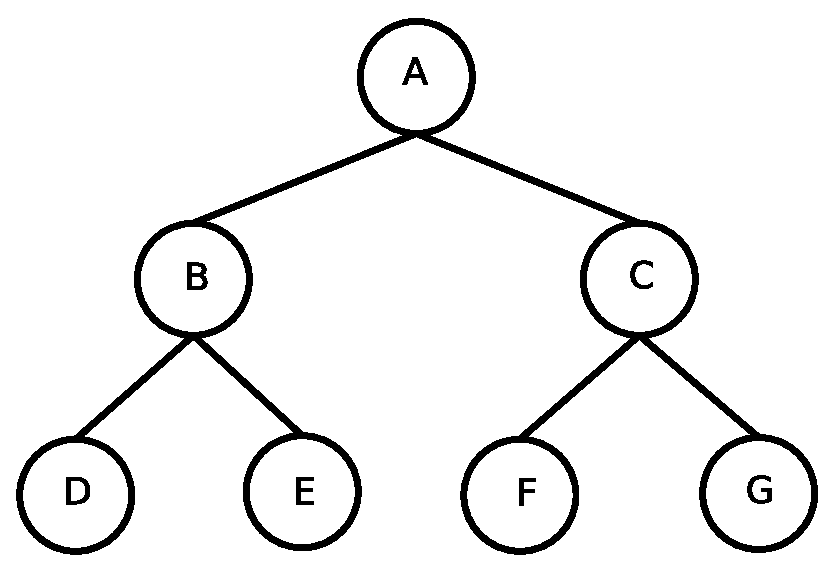
\includegraphics[width=0.4\textwidth]{chap02/dfs}
\caption{深度优先与广度优先}
\label{fig:dfs}
\end{figure}

迭代环计数算法也依赖于点---边关系矩阵,该算法利用了深度优先算法的思想,主要步骤为:
\begin{enumerate}
\item 初始化一个结点作为树的根。
\item 找到与这个结点相邻的结点,并把其中一个结点作为根的子结点,放入树的第二层。
\item 继续找与第二层中的点相邻的一个结点,作为树的第三层。在搜索根的子结点的相邻点的过程中,要排除其上一层中的点,即根结点不作为树的第三层中的点。
\item 若路径中包含两个相同的结点,则说明这个路径中的结点形成一个环,并继续按照点边关系寻找下一个结点。
\item 若没有环形成,则继续寻找下一个结点,并更新路径。
\item 若这条路径已经到最后一个结点,则回到树的上一层并更新路径。
\item 重复2到6步直到第8步完成。
\item 如果当前结点不是第一个结点,并且所有的结点都已搜索到则算法结束。
\end{enumerate}

如图\ref{fig:graph-tree},a表示一个图,b是根据迭代环计数算法转换成的树。首先初始化一个点1作为树的根,根据点边关系矩阵,搜索到1的子结点2,放入树的第二层,根据2的点边关系矩阵,搜索到3结点,放入树的第三层,继续搜索3的点边关系矩阵,得到结点1,此时结点1、2、3、1形成一个环结构,然后回溯到1的上一层,即第三层继续寻找除1以外与3相连的其他点,即4点,然后继续搜索,直到遍历所有的点边关系矩阵。由此,遍历结束后,得到三个环结构,即123、1243、243。重复搜索的环将在遍历结束后被去除。
\begin{figure}[H]
\centering
  \begin{minipage}[b]{0.48\textwidth} 
      \centering 
      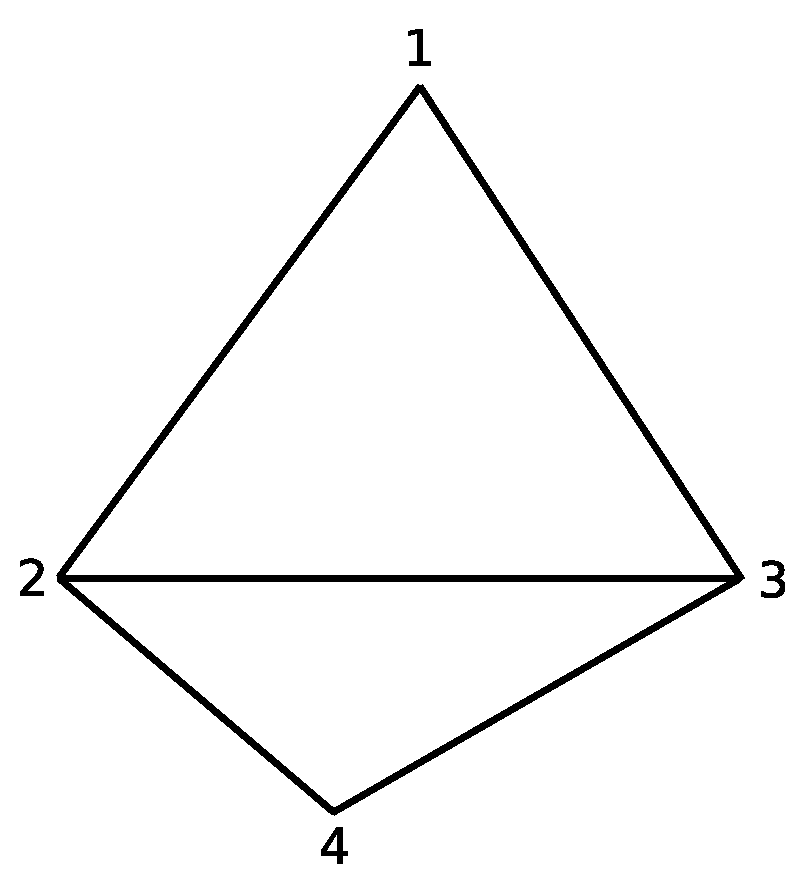
\includegraphics[width=4cm]{chap02/loop}
        \centerline{(a)图}\medskip
    \end{minipage}
  \begin{minipage}[b]{0.48\textwidth}
    \centering
    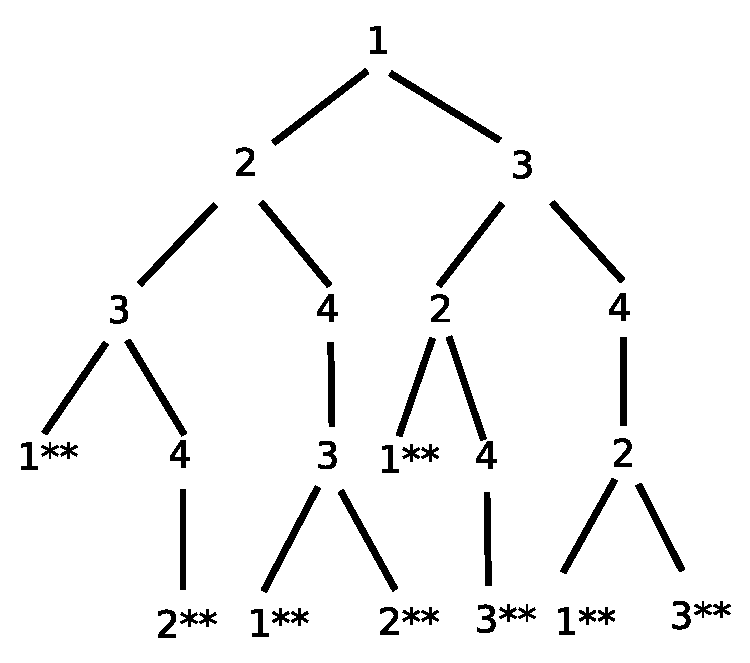
\includegraphics[width=5cm]{chap02/graph-old}
      \centerline{(b) 树}\medskip
  \end{minipage}
\caption{图与迭代环计数算法转化树}
\label{fig:graph-tree}
\end{figure}

由此可知,迭代环计数算法能够检测到图中的所有环,不仅包括最小环,还存在由最小环形成的大环。在图像中,我们感兴趣的是提取图像中的最小环结构。并且当图像中的环结构较多,点边关系错综复杂时,深度优先算法的搜索路径往往容易变得冗长,且迭代环计数算法的搜索路径容易重复,从而增加算法复杂性。

基于此,我们提出了基于广度优先检索策略的环结构检测算法,使得树结构更加简单,从而减小算法的复杂性。算法思想同样是把图变换成一颗树,但是基于广度优先算法,并且增加了对于兄弟结点的考虑,从而降低算法的复杂性,其主要步骤为:
\begin{enumerate}
\item 初始化一个结点作为树的根。
\item 找到与这个结点相邻的所有结点,并把他们作为根的子结点,放入树的第二层。相邻的点可以通过点边邻接矩阵得到,因为它列出了与某一点相邻的所有的结点。
\item 判断当前层是否有相邻的兄弟结点或相同的结点,若有,则说明有环形成。回到上一层,找到其相同的父结点或相邻的不同的父结点,若没有找到,则继续回到上一层,直到找到为止,那么,搜索路径上的点就可以组成环。
\item 继续检测与当前层的结点相连的除父结点及兄弟结点以外的其他结点并放入树的下一层。然后转入第三步,直到所有的点边关系遍历结束。
\end{enumerate}
经过以上步骤,所有三点、四点、五点环将被检测到。如图\ref{fig:cycle-tree}(a)是一个图的例子,图中有一个三点环、一个四点环、一个五点环。通过我们的环结构检测算法,这三个环要被准确无误的检测出来。首先确定$v_1$为初始点,即树的根。通过点边关系可得,与之相邻的点分别为$v_2, v_5, v_6, v_8$,于是,这四个点将被当作根的子结点放入树的第二层。判断这四个点是否有相邻点,发现$v_5, v_6$是相邻的,那么$v_5, v_6$及其相同的父结点$v_1$形成一个三点环,继续寻找这四个点的相邻点(除父结点及兄弟结点以外),放入树的第三层。判断这些点有没有相邻点或相同点。通过点边关系矩阵发现$v_3,v_4$是相邻点,那么$v_3,v_4$与其父结点$v_2,v_5$及其父结点的相同父结点$v_1$形成五点环,同理,$v_{1}v_{6}v_{7}v_{8}$组成四点环。至此,所有的搜索都已完成,即共找到三个环,$v_{1}v_{5}v_{6}$组成三点环,$v_{1}v_{6}v_{7}v_{8}$组成四点环,$v_{1}v_{2}v_{3}v_{4}v_{5}$组成五点环。

\begin{figure}
\centering
  \begin{minipage}[b]{1\textwidth} 
      \centering 
       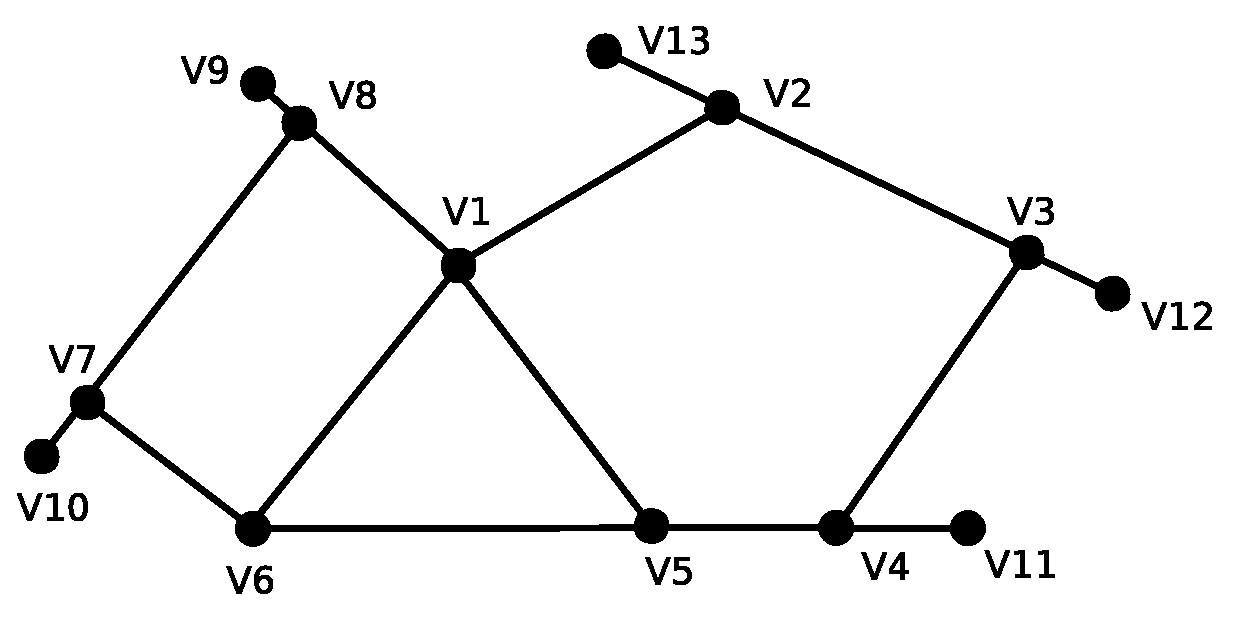
\includegraphics[width=7cm]{chap02/graph2}
       \centerline{(a)}\medskip
    \end{minipage}
  \begin{minipage}[b]{1\textwidth}
    \centering
    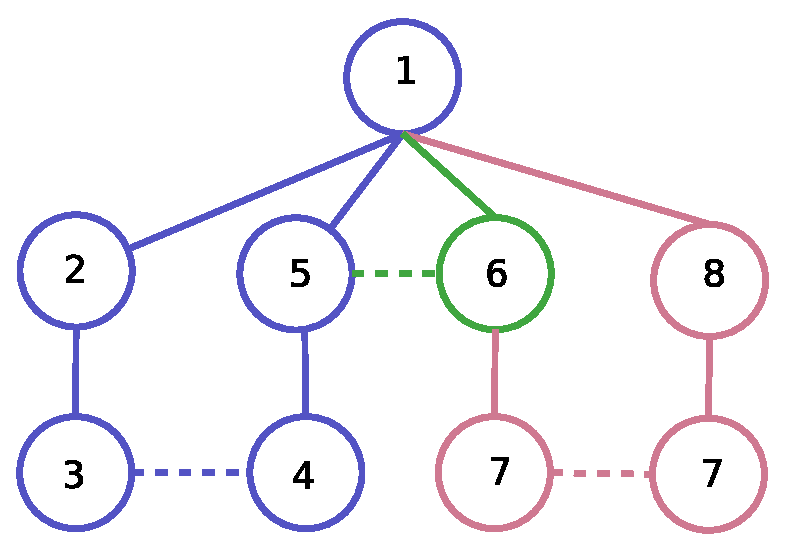
\includegraphics[width=6cm]{chap02/tree}
    \centerline{(b)}\medskip
  \end{minipage}
\caption{图与搜索树}
\label{fig:cycle-tree}
\end{figure}

通过我们提出的环结构检测算法算法,图\ref{fig:graph-tree}(a)可以转化为图\ref{fig:simple-tree}中的树,由此可以看到,相比图\ref{fig:graph-tree}(b)中的树,图\ref{fig:simple-tree}更加的简单,搜索路径不会重复,算法更加高效。

\begin{figure}
\centering
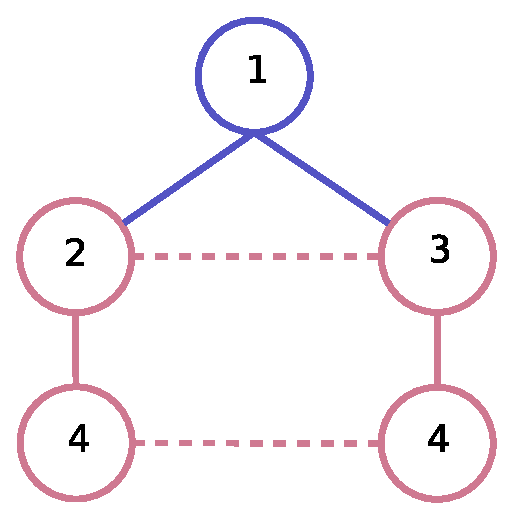
\includegraphics[width=0.3\textwidth]{chap02/simple-graph}
\caption{图\ref{fig:graph-tree}(a)的搜索树}
\label{fig:simple-tree}
\end{figure}


\section{环结构描述}
\label{}
环之所以能用在图像识别与匹配领域,是因为它是稳定的显著的特性。而它的稳定性与显著性则体现在用来描述环结构的特征向量上。

一个环结构是由一系列分叉点与连接这些分叉点之间的线组成。我们用分支角度与分支长度来描述环结构。以任意分叉点$v_i(x_0, y_0)$为中心,构造一个$7 \times 7$的邻域。记录分支与邻域边缘24个像素相交点的坐标,假设其坐标值为$x_j, y_j, j=1, 2, \ldots$。则分支方向为:
\begin{align}
\beta_j = arctan\frac{dy}{dx}, dy = y_j - y_0, dx = x_j - x_0 
\end{align}

由于arctan的取值范围为$-90^{\circ} \sim 90^{\circ}$,故还需保证求出的角度大于0。即
\begin{align}
\alpha_j = \left\{ \begin{array}{ll}
\beta_j & \textrm{$dy \geq 0$, $dx \geq 0$} \\
\beta_j + 180^{\circ} & \textrm{$dy \geq 0$, $dx \leq 0$ 或 $dy \leq 0$, $dx \geq 0$}\\
\beta_j + 360^{\circ} & \textrm{$dy \leq 0, dx \leq 0$}
\end{array} \right.
\end{align}
邻域边缘24个像素把$360^{\circ}$分成了24个离散值,每个相邻的分支角度相差$15^{\circ}$。每个角度以水平线为基准,故分叉点之间的角度值可通过式\ref{eq:Angle}计算:
\begin{align}
\theta_i = \alpha_{i+1} - \alpha_i, \qquad
\theta_i = \left\{ \begin{array}{ll}
\theta_i + 360^{\circ} & \theta_i \le 0 \\
\theta_i & \theta_i \geq 0
\end{array} \right.
\label{eq:Angle}
\end{align}
如图\ref{fig:calculate-angles},以三分叉点为中心划定一个$7\times7$邻域,邻域的边缘24个像素把$360^{\circ}$分为24个方向的角度,分别为$15^{\circ}, 30^{\circ},45^{\circ}, \ldots, 360^{\circ}$。在这个邻域的边缘24个像素中,像素值为1的像素以水平线为基准与中心像素形成分支角度,图\ref{fig:calculate-angles}中,共形成3个角度,即$45^{\circ}, 150^{\circ},270^{\circ}$,则分支之间的角度为$105^{\circ}, 120^{\circ}, 135^{\circ}$。

\begin{figure}[H]
\centering
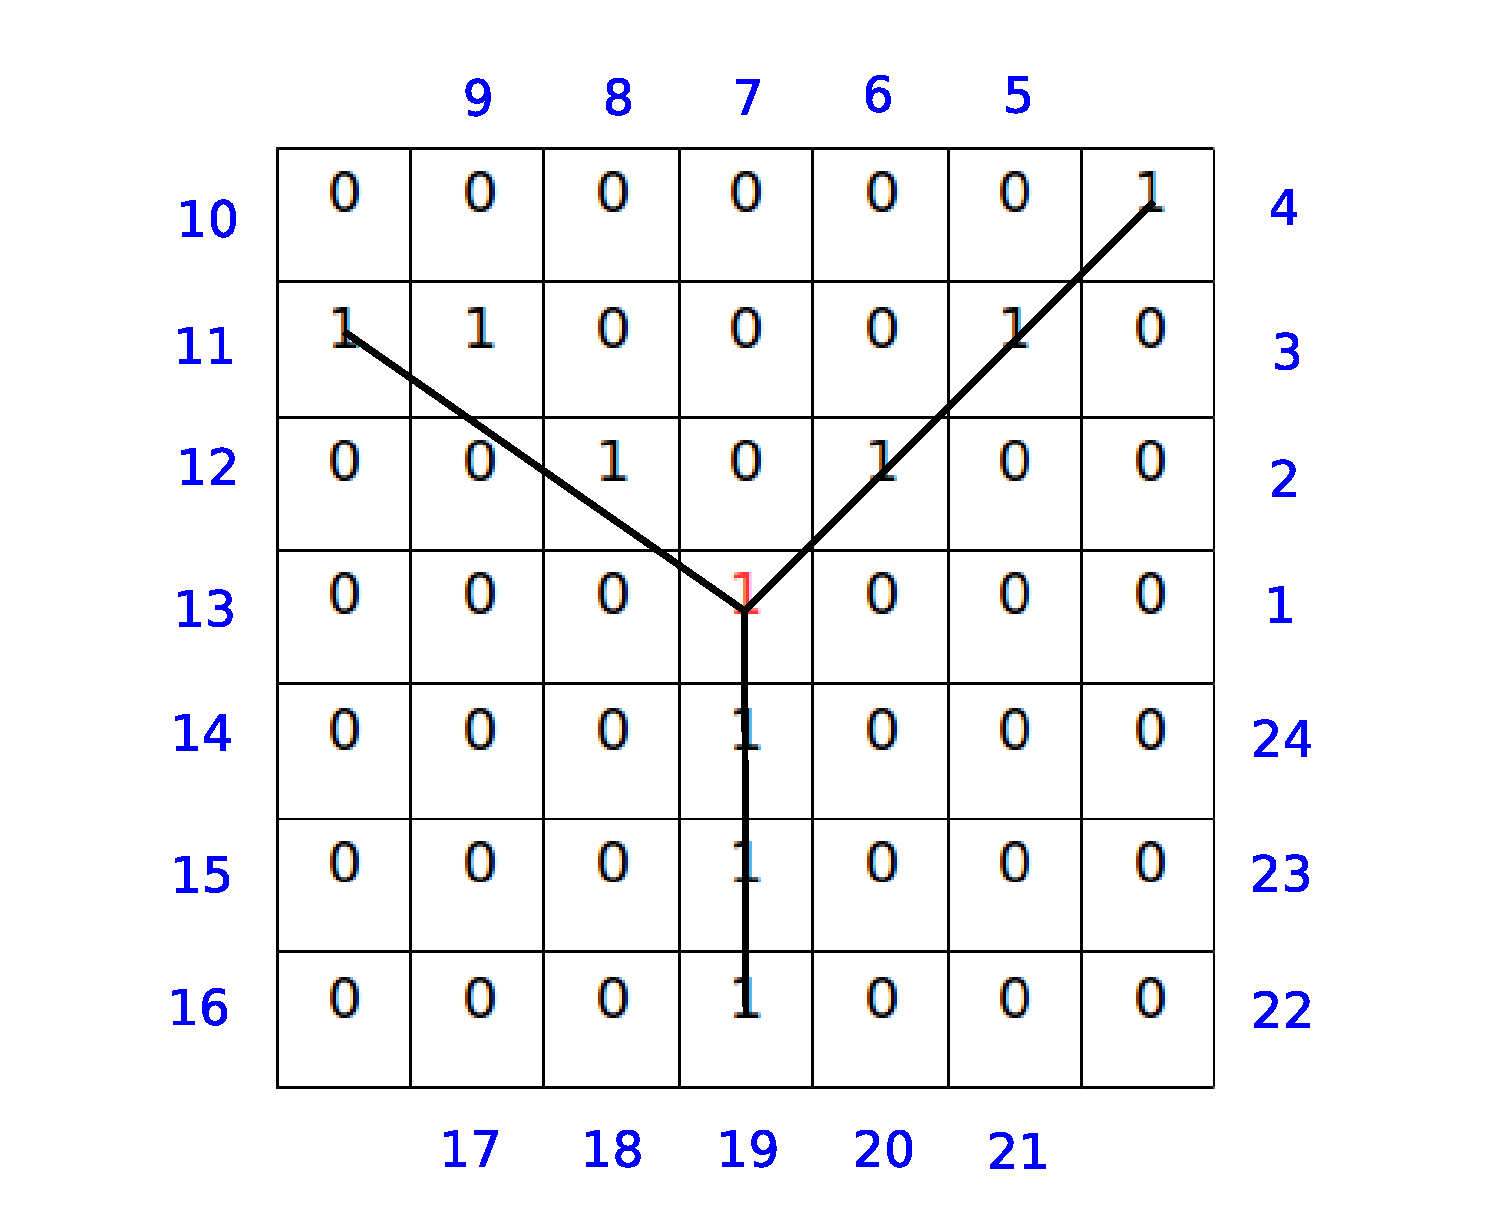
\includegraphics[width=0.5\textwidth]{chap02/7-7}
\caption{分支角度计算}
\label{fig:calculate-angles}
\end{figure}

分叉点之间的分支长度为分叉点之间的欧式距离,即:
\begin{align}
L = \sqrt{(y_j - y_0)^2 + (x_j - x_0)^2}, j = 1, 2, \ldots
\end{align}

归一化属于数字信号处理范畴,即将有量纲的表达式,经过变换,转换为无量纲的表达式,成为标量。它是简化计算,缩小量值的有效办法。而对于环结构特征,通过归一化,能使在减少计算量的基础上,使环结构特征具有平移、旋转及尺度不变性。图\ref{fig:description}给出了四点环结构示意图,角度归一化、长度归一化及最终产生的特征向量可分别用式\ref{eq:angle}、式\ref{eq:length}及式\ref{eq:vector}表示。$L_{1} \sim L_{4}$,$\theta_{1} \sim \theta_{14}$,$\theta_{15} \sim \theta_{18}$ 分别代表分支长度、分支角度及分叉点之间的角度。

\begin{figure}[H]
\centering
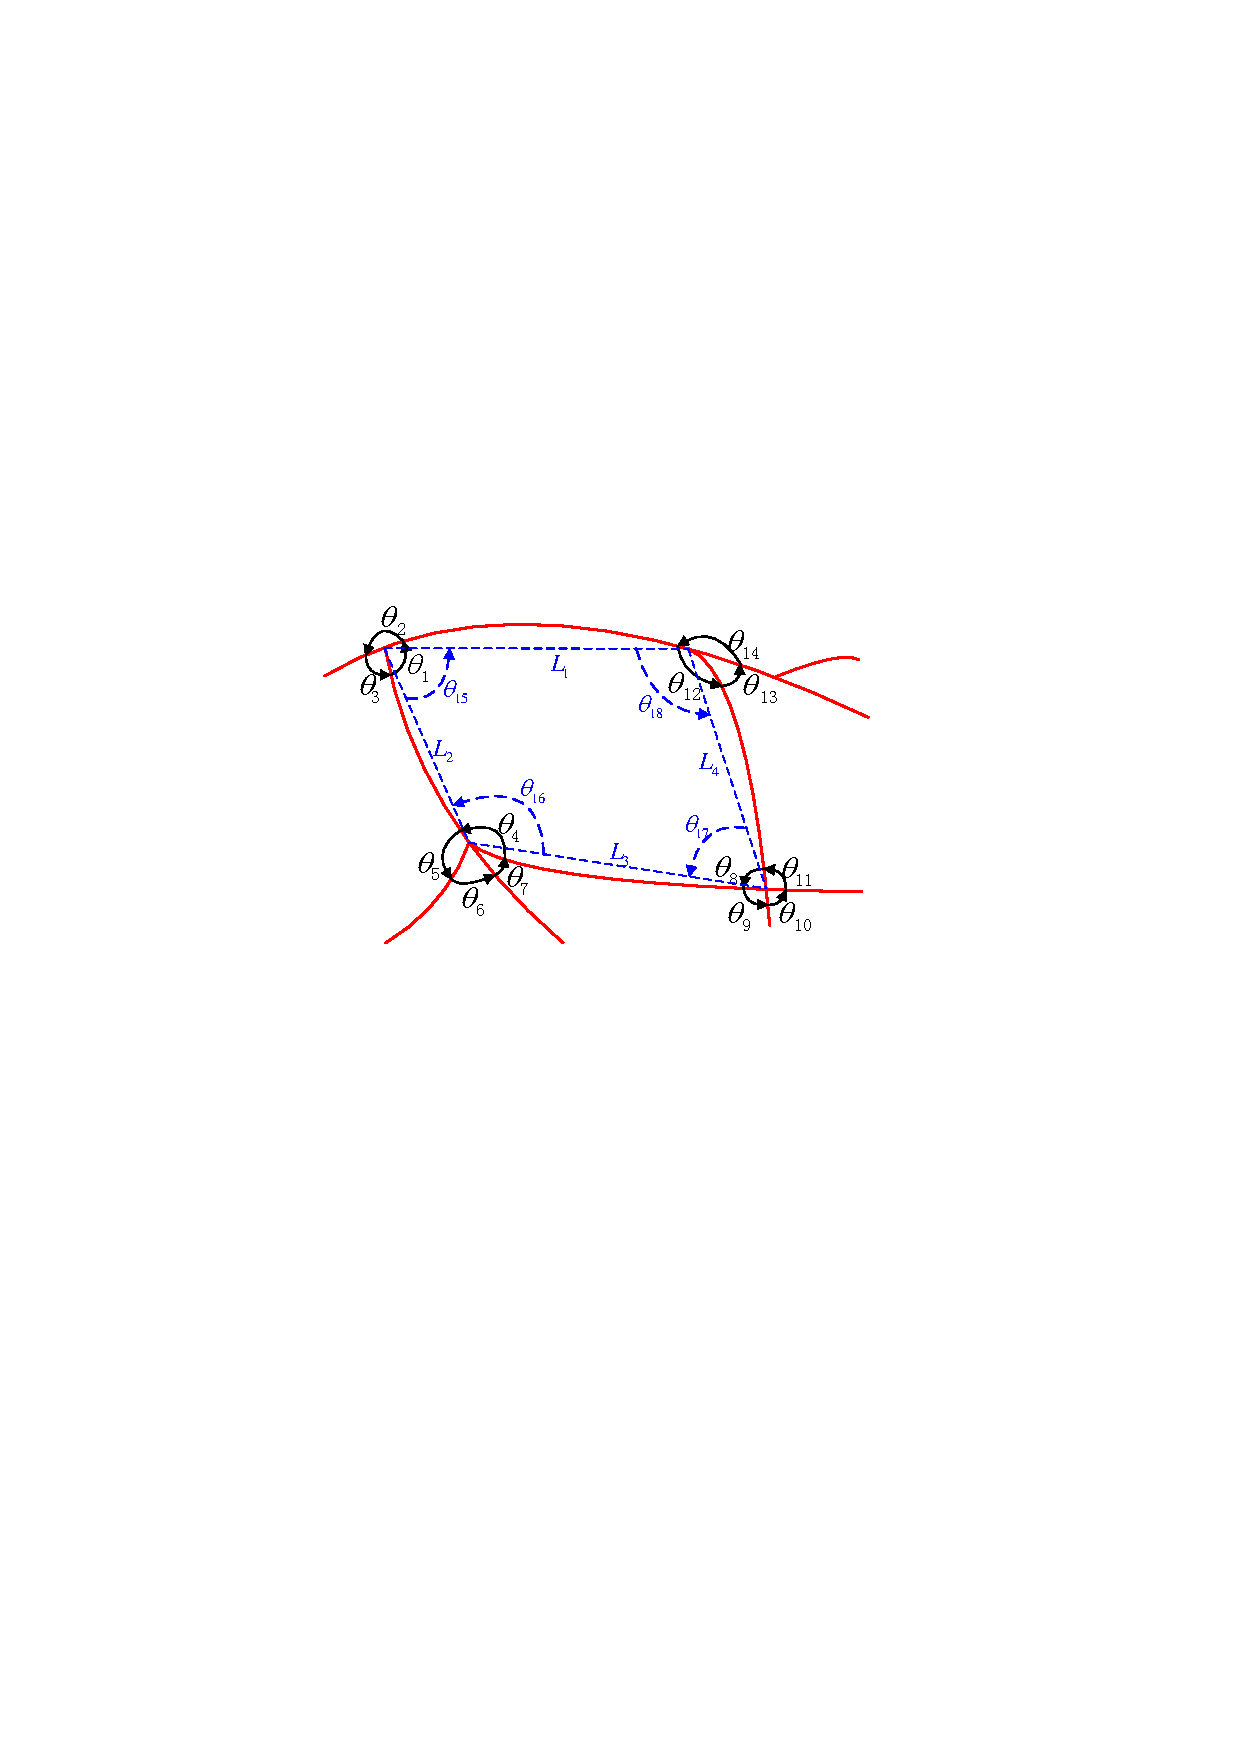
\includegraphics[width=0.4\textwidth]{chap02/description.pdf}
\caption{环结构描述}
\label{fig:description}
\end{figure}
\begin{align}
L_{iNorm}&=\frac{L_i}{\sum{L}}\label{eq:length}\\
\theta_{jNorm}&=\frac{\theta_j}{360^\circ}\label{eq:angle}
\end{align}
\begin{multline}
\tilde{v}=\{\textrm{角度,长度}\}=\{L_{1},L_{2},L_{3},L_{4},\theta_{1},\theta_{2},\theta_{3},\mathbf{0},\theta_{4},\\\theta_{5},\theta_{6},\theta_{7},\theta_{8},\theta_{9},\theta_{10},\theta_{11},\theta_{12},\theta_{13},\theta_{14},\mathbf{0},\theta_{15},\theta_{16},\theta_{17},\theta_{18}\}
\label{eq:vector}
\end{multline}

值得注意的是,组成环的分叉点个数不一样,并且每个分叉点的分叉角度也不同,这就导致了不同类型的环有不同长度的特征向量。为了便于识别和配准的需要,我们可根据实际情况设定一个角度个数标准,比如说,若设置4个分支角度为标准,那么小于4个角度的分叉应用0来补齐,这样就保证同种类型的环的特征向量的长度是相同的。这样,当用来做配准或识别时,就可匹配同种类型的环的特征向量来达到目的。

\section{本章小节}
\label{}

本章介绍了环结构特征的定义、特点及应用,阐述了从图像中检测环的主要步骤:检测分叉点及其连接关系、滤除无效分叉点、检测环结构,并重点介绍了我们提出的环结构检测算法。同时,结合环结构的特点,给出了特征描述的方法。通过把环结构特征表示成为特征向量,就能为下一步的配准、识别奠定基础。


%%% Local Variables: 
%%% mode: latex
%%% TeX-master: t
%%% End: 

\chapter{环结构在视网膜图像配准中的应用}
\label{cha:intro}


\section{视网膜图像配准研究现状}
\label{}

视网膜是人类的重要视觉器官,通过观察视网膜血管图像,医生能诊断和治疗眼底循环障碍疾病以及全身性疾病,比如青光眼、白内障、糖尿病等。但由于成像条件的限制,视网膜图像表现出中间亮、四周暗、对比度弱、有强噪声干扰的特点,可能会导致医生误诊。因此,通过图像处理与分析技术对视网膜图像进行质量改善、图像配准等自动分析,对疾病的诊断和治疗有着非常重要的价值。

视网膜配准技术是辅助眼科诊断和治疗的关键技术。视网膜血管图像通常是在不同时间或角度下获取的,包含有价值的时间与局部信息。通过视网膜配准技术,将多幅同一个个体的图像变换到同一幅图像中,就可以更加全面的显示视网膜特征,从而帮助医生进行比较和分析以选择合适的治疗方案。

目前,国内外有大量的视网膜图像配准相关的研究工作,主要可以分为两类:基于强度的视网膜图像配准与基于特征的视网膜图像配准\cite{oliveira2014medical}。

基于强度的视网膜配准方法通常基于互相关、相位相关、互信息\cite{penney1998comparison}等选择合适的相似性度量~\cite{Glocker02,Nunes03,Dreo04}。这些方法需要整合整幅图像的信息来完成配准,找到最佳的解决方案需要很大的计算成本。同时,基于强度的对准方法在图像质量较低或重叠区域较小的时候容易失败。这就刺激了基于特征的图像配准的发展。

基于特征的图像配准将对整个图像的分析转化为对图像特征的分析\cite{dingnan},因此,图像特征的选取是基于特征的方法中的关键问题。分叉点是视网膜血管的显著特征,大多数基于特征的图像配准把分叉点特征作为主要特征来进行特征匹配。Zana和Klein\cite{zana1999multimodal}利用分叉点及其周围的血管方向来做配准。Can和Stewart\cite{can2002feature}提出基于分叉点和交叉点的分层算法,能够在一定程度上减少特征错配。2003年,这一思想又进行了进一步的扩充,逐渐发展为双引导的迭代最近点算法\cite{stewart2003dual},它利用一种从简单到复杂,从局部到全局的策略最终确定最优的变换模型。Lalibert\cite{laliberte2003registration}等提出利用血管分叉点作为控制点来估计变换模型并利用了像素级的融合技术。Chanwimaluang\cite{chanwimaluang2006hybrid}等结合了基于区域和基于特征的方法,利用分叉点和交叉点来进行配准。Perez-Rovira\cite{perez2012rerbee}等提出了REES方法,利用分叉点和血管段来配准。这些方法很大程度上取决于单个分叉点的分支角度,但角度信息的精度不高容易引起分叉点错配,从而导致配准的失败。

与上述方法相比,基于结构的配准方法更容易克服错配的情况。Chen\cite{chen2011retinal,chen2015retinal}等人提出了基于分叉结构的配准方法,分叉结构由一个主分叉点和与它相连的三个相邻分叉点组成,归一化的分支角度和长度作为特征向量,一定程度上解决了错配的难题。Shen\cite{shen2012blood}等人扩展了基于分叉结构的配准方法,利用局部的精细配准来纠正配准精度。然而,若是血管树十分复杂,分叉结构特征仍然不够独特和可靠,因为复杂的血管树会使得匹配的血管丢失。

鉴于此,我们提出了基于环结构特征的从全局到局部的视网膜图像配准方法。环结构由血管分叉点和交叉点及与它们相连的血管组成。这一特征对于视网膜血管来说更加唯一和可靠,故它同样可应用于其他的领域,比如视网膜识别等。为了克服对视网膜分割结果的依赖性,我们采用多小波核多层分解方法,从而产生多尺度的血管树。不同尺度的血管树所代表的分割的精细程度不同。然后我们提出了动态路径移动算法来提取由多个不同数量的分叉点组成的多环特征,归一化的分支角度和长度来作为特征向量,采用相似性度量来进行全局初次配准。对于远离匹配特征的区域,我们采用局部分叉点信息来纠正配准精度。最后,我们采用骨架化对准精度来优化特征和尺度的选择,基本流程如图\ref{fig:framework}。
\begin{figure}[!ht]
  \centering
  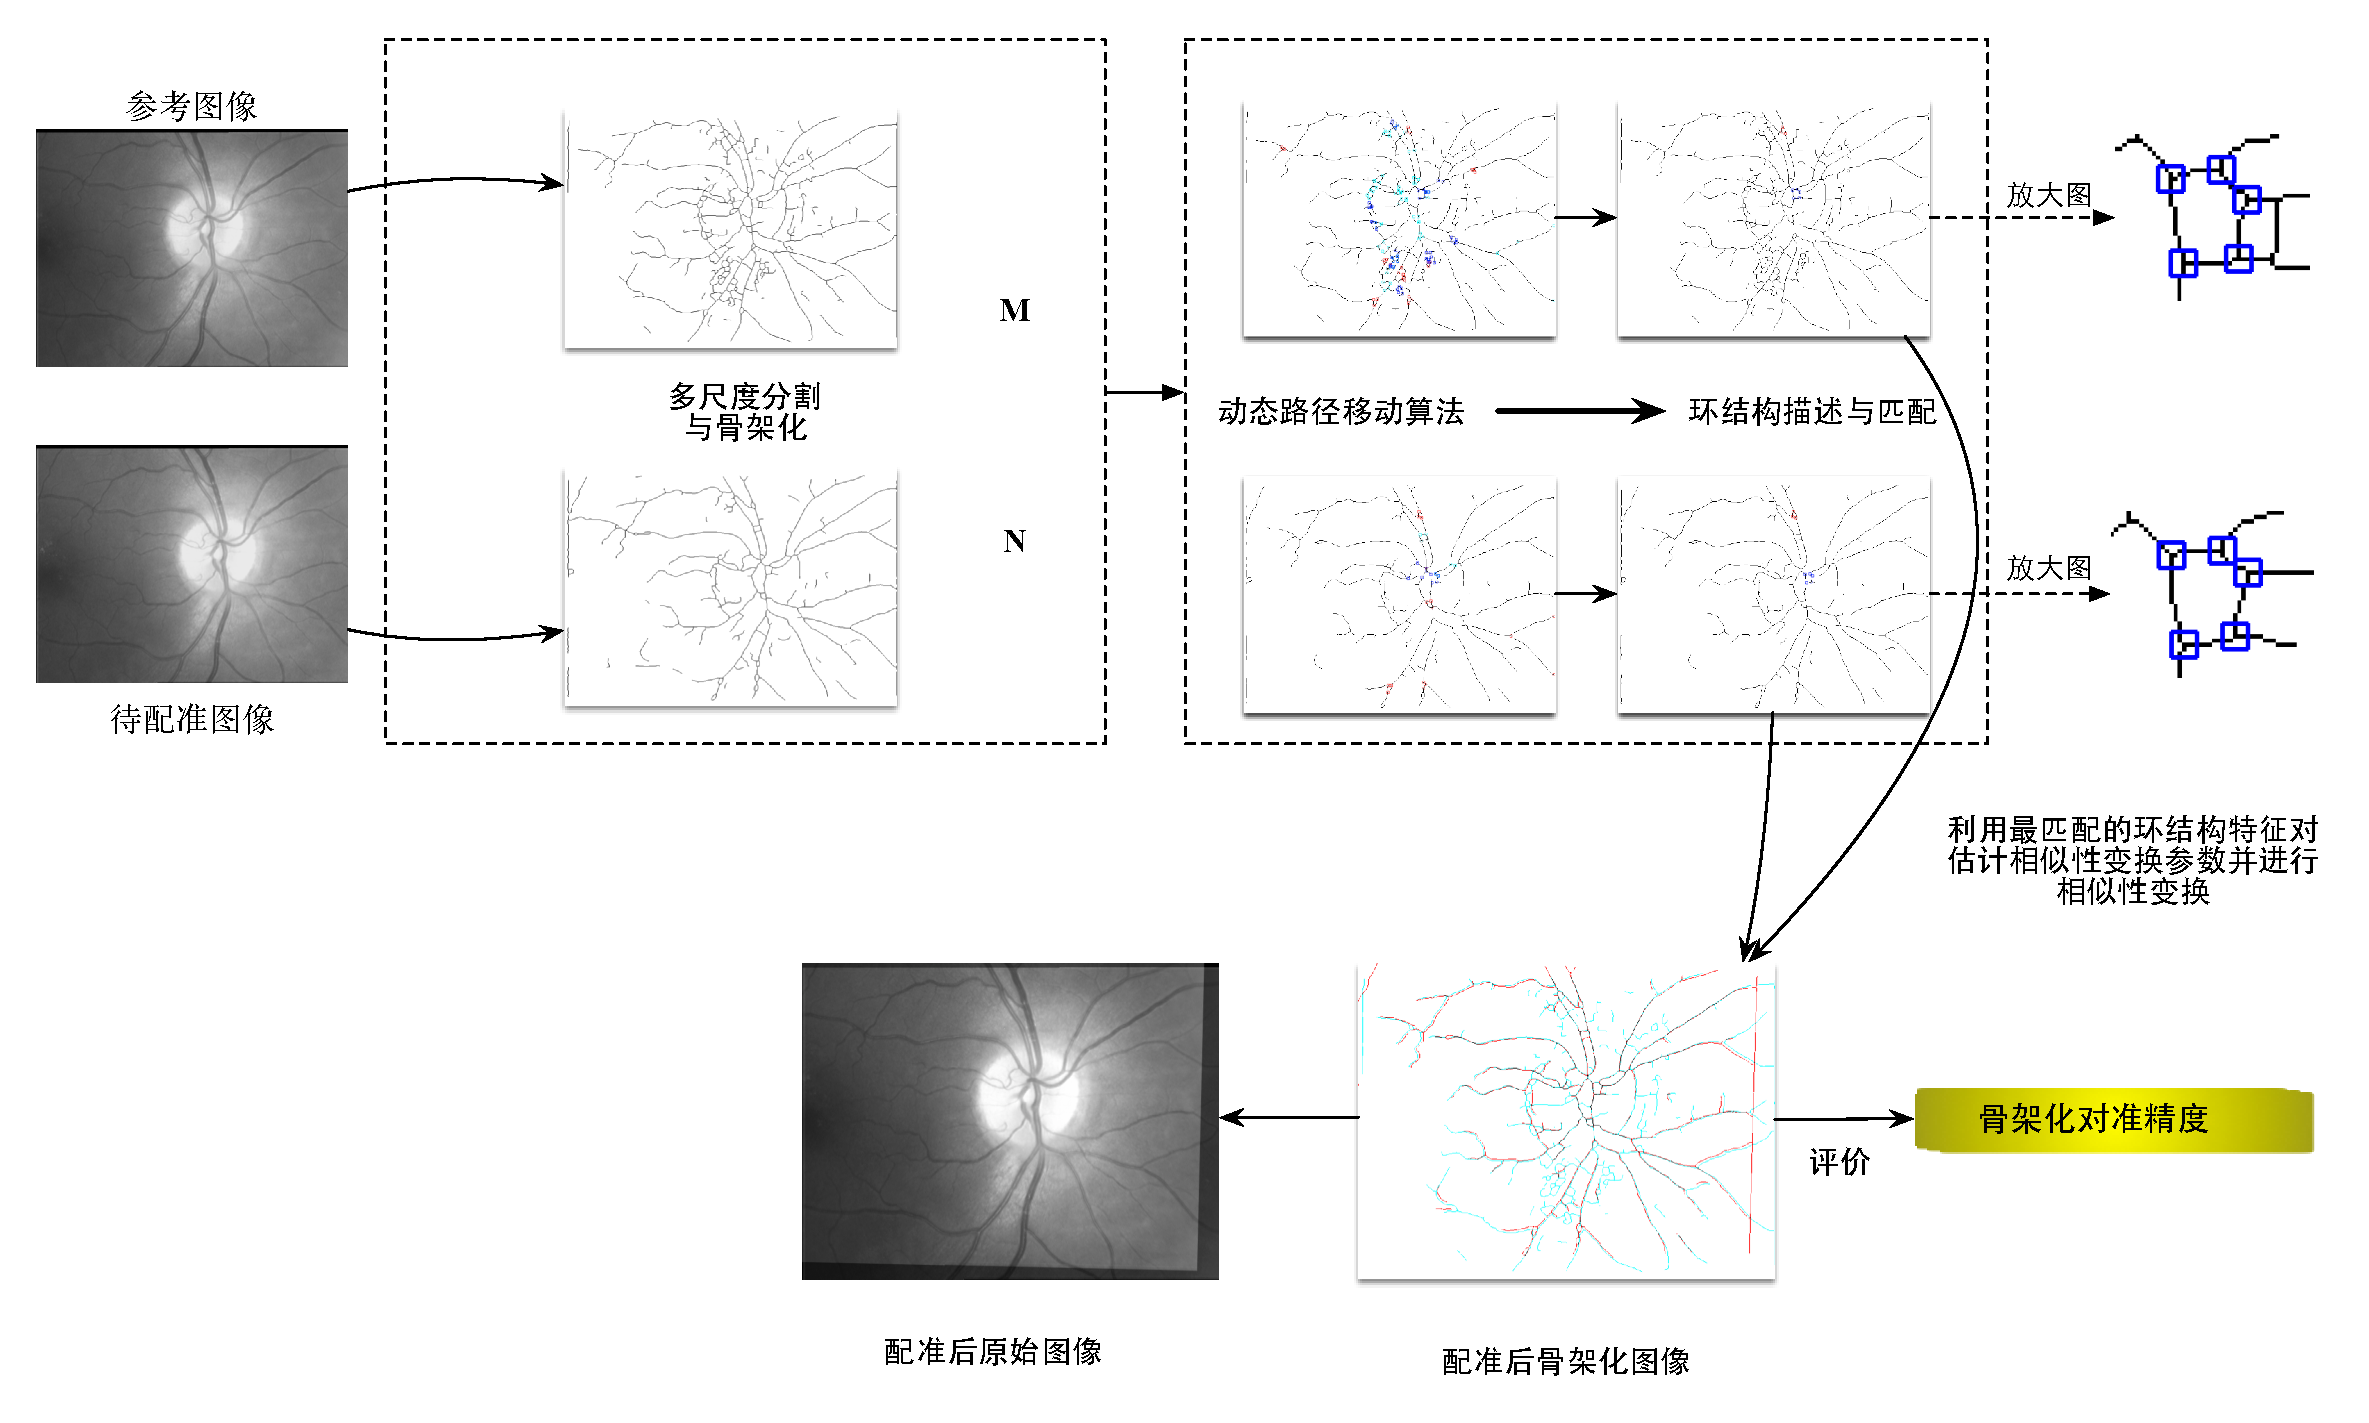
\includegraphics[width=1\textwidth]{chap03/framework}
  \caption{基本框架}
  \label{fig:framework}
\end{figure}


由第\ref{cha:cycle}章可知,采用多小波核多层分解方法,可以产生多尺度的血管树,为了确保配准的精度,我们选择了14个尺度的血管树,分别提取每个血管树中的环结构,描述成特征向量。这样,一幅图像则有14组特征向量。

视网膜图像配准是指将不同角度和时间获取的两幅同一个个体的图像变换到一幅图像中。两幅图像进行配准,即是$14 \time 14$组特征向量之间的匹配。我们采用相似性度量来寻找两幅图像特征向量之间的匹配对。

\section{相似性度量}
\label{cha:similarity}

假设参考图像的某一尺度与待配准图像的某一尺度分别有$m$和$n$组环结构特征,则他们之间的相似性测度为
\begin{align}
D_{pq} = mean(|V_p-W_q|), p = 1, 2, \ldots, m; q = 1, 2, \ldots, n
\end{align}
其中,$V_p$和$W_j$分别表示参考图像和待配准图像的第$p$个和第$q$个环结构。相似性测度越小,说明两个环结构越相似。为了保证最小的相似性测度相对应的环特征结构是匹配正确的,我们选择一个固定阈值来确保准确性,若最小测度仍大于这个阈值,我们认为这对环结构仍是不匹配的。

通过观察发现,视网膜血管图中,由三个分叉点、四个分叉点、五个分叉点组成的环居多,为了减小算法的复杂性,我们只选择三点环、四点环、五点环来作为特征。因此,相似性度量只在同种类型的环之间进行计算,得到最匹配的环结构。这种方法虽然可能丢失一些特征,但更能保证匹配的准确性且减小算法的复杂性。

\section{相似性变换}
\label{}

要使一幅图像变换到另一幅图像中,就要采用几何变换模型进行变换。几何变换模型是指坐标空间或图像 的像素值转换到另一个坐标空间或像素值的变换。常见的变换方式有平移、缩放、旋转、翻转、转置等。常用的空间变换模型有相似性变换、仿射变换、二次多项式变换等。

\begin{enumerate}
\item 平移,是指在一个平面内,将一个图像上的所有点都按照某个方向做相同距离的移动。平移不会改变图像的大小和形状。图像经过平移,对应角相等、对应线段相等、对应点所连的线段相等。它可视为同一个向量加到每个点上或将坐标系统的中心移动一定距离的结果。平移的方向不限于水平,也可为其它方向。设$(x_0,y_0)$是原图像上的一点,若将该图像沿水平方向平移tx,垂直方向平移ty,若平移后的坐标变为$(x_1,y_1)$,则其变换公式为:
\begin{align}
\left[ \begin{array}{c}
x_1 \\
y_1 \\
1   
\end{array} \right]
=
\left[ \begin{array}{ccc}
1 & 0 & tx \\
0 & 1 & ty \\
0 & 0 & 1
\end{array} \right]
\left[ \begin{array}{c}
x_0 \\
y_0 \\
1
\end{array} \right]
\end{align}
\item 在平面内,把一个图像绕一个定点沿某个方向转动一个角度,这样的变换叫做旋转。设$(x_0,y_0)$是原图像上的一点,若绕(0, 0)点旋转$\theta$角后,坐标变为$(x_1,y_1)$,则其变换矩阵为:
\begin{align}
\left[ \begin{array}{c}
x_1 \\
y_1 \\
1   
\end{array} \right]
=
\left[ \begin{array}{ccc}
cos\theta & sin\theta & 0 \\
-sin\theta & cos\theta & 0 \\
0 & 0 & 1
\end{array} \right]
\left[ \begin{array}{c}
x_0 \\
y_0 \\
1
\end{array} \right]
\end{align}
\item 缩放,即图像按一定的比例进行一定程度的放大或缩小。设图像在x轴方向的缩放比例为fx,在y轴方向的缩放比例为fy,则原图像中点$(x_0, y_0)$经缩放后的坐标变为$(x_1, y_1)$,则其变换矩阵为:

\begin{align}
\left[ \begin{array}{c}
x_1 \\
y_1 \\
1   
\end{array} \right]
=
\left[ \begin{array}{ccc}
fx & 0 & 0 \\
0 & fy & 0 \\
0 & 0 & 1
\end{array} \right]
\left[ \begin{array}{c}
x_0 \\
y_0 \\
1
\end{array} \right]
\end{align}
\item 由一个图像改变为另一个图像,在改变过程中保持形状不变的变换叫做相似变换。相似变换不改变图像中每一个角的大小,任何相似变换可以分解为缩放、平移、旋转和翻转的组合。相似性变换可定义为:
\begin{align}
X&=xs\cos\varphi-ys\sin\varphi+a\\
Y&=xs\sin\varphi+ys\cos\varphi+b
\end{align}
$s$代表缩放尺度,$\varphi$表示旋转角度,$(a, b)$表示参考图像与待配准图像的平移变化。
\item 仿射变换是图像平移、旋转、缩放、翻转、错切的复合。仿射变换可以用表示为:
\begin{align}
T = \left[ \begin{array}{ccc}
1 & 0 & 0 \\
0 & 0 & 0 \\
a & b & 0
\end{array} \right]
\times
\left[ \begin{array}{ccc}
1 & 0 & 0 \\
0 & 0 & 0 \\
-x & y & 0
\end{array} \right]
\times
\left[ \begin{array}{ccc}
cos\varphi & sin\varphi & 0 \\
-sin\varphi & cos\varphi & 0 \\
0 & 0 & 0
\end{array} \right]
\times
\left[ \begin{array}{ccc}
1 & 0 & 0 \\
0 & 0 & 0 \\
c & d & 0
\end{array} \right]
\label{eq:affine}
\end{align}
其中,$(a, b)$为图像的水平垂直平移量,$\varphi$表示旋转角度,$(x, y)$表示参考图像中的坐标点,$(c, d)$为旋转后的中心坐标。

仿射变换有六个自由量,六个自由量与六个可以变换的参数相对应,于是,将式\ref{eq:affine}变换可得
\begin{align}
X = a_1x + a_2y + a_3, 
\qquad
Y = a_4x + a_5y + a_6
\end{align}
仿射变换的主要特征是保持直线平行性和像素点的共线性。比如在进行映射时,即第一幅图像上的直线映射到第二幅图像上也是直线,方向不发生变化,但长度可能发生变化。
\item 假设三位空间中$P=(X, Y, Z)^T$和$Q=(X_1,Y_1,Z_1)^T$分别表示两幅图像中相应点的空间坐标,则空间中二次变换模型坐标为:
\begin{align}
Z = A_1X^2 + A_2XY + A_3Y^2 + A_4X + A_5Y + A_6
\label{eq:twice-4}
\end{align}
空间中刚体变换模型为
\begin{align}
\left[ \begin{array}{c}
X_1\\
Y_1\\
Z_1
\end{array} \right]
=
\left[ \begin{array}{ccc}
r_{11} & r_{12} & r_{13} \\
r_{21} & r_{22} & r_{23} \\
r_{31} & r_{32} & r_{33}
\end{array} \right]
\left[ \begin{array}{c}
X \\
Y \\
Z
\end{array} \right]
+
\left[ \begin{array}{c}
t_x \\
t_y \\
t_z
\end{array} \right]
\label{eq:twice-1}
\end{align}
其中,$r_{ij}$为空间正交变换矩阵的参数,$(t_x, t_y, t_z)$为空间平移参数,图像二维平面与三维空间之间的转换公式为:
\begin{align}
\left[ \begin{array}{c}
X \\
Y 
\end{array} \right]
=
\left[ \begin{array}{c}
\frac{sx-c_x}{a_x} \\
\frac{sy-c_y}{a_y}
\end{array} \right]
\label{eq:twice-2}
\end{align}
\begin{align}
Z = a_1x^2 + a_2xy + a_3y^2 + a_4x + a_5y + a_6
\label{eq:twice-3}
\end{align}
其中,$(a_x, a_y)$为尺存参数,s为图像的缩放比例,$(c_x, c_y)$为图像中心点的坐标。

将\ref{eq:twice-1}、\ref{eq:twice-2}、\ref{eq:twice-3}代入\ref{eq:twice-4}得:
\begin{align}
\left[ \begin{array}{c}
X_1 \\
Y_1
\end{array} \right]
=
\left[ \begin{array}{c}
r_{11}\frac{sx-c_x}{a_x} + r_{12}\frac{sy-c_y}{a_y} + r_{13} \\
(a_1x^2 + a_2xy + a_3y^2 + a_4x + a_5y + a_6)\\
r_{21}\frac{sx-c_x}{a_x} + r_{22}\frac{sy-c_y}{a_y} + r_{23}\\
(a_1x^2 + a_2xy + a_3y^2 + a_4x + a_5y + a_6)
\end{array} \right]
\label{eq:twice-5}
\end{align}
将\ref{eq:twice-5}变换到二维平面,可得12个自由参数,分别用$\theta_1 \sim \theta_{12}$代替,可得:
\begin{align}
\left[ \begin{array}{c}
x_1 \\
y_1
\end{array} \right]
=
\left[ \begin{array}{cccccc}
\theta_{11} & \theta_{12} & \theta_{13} & \theta_{14} & \theta_{15} & \theta_{16} \\
\theta_{21} & \theta_{22} & \theta_{23} & \theta_{24} & \theta_{25} & \theta_{26} 
\end{array} \right]
\left[ \begin{array}{c}
x^2, xy, y^2, x, y, 1
\end{array} \right]^T
\end{align}
通常情况下,高阶多项式通常不用于实际应用,因为利用高阶多项式进行配准时,在远离特征区域的地方,可能会造成不必要的变形。一般来说,特征的数目要多于决定映射函数所需要的最小数量。映射函数的参数通过最小二乘拟合方法计算,所以,多项式使得在特征周围的最小平方误差最小。但这样的映射对于远离特征周围的区域并不适用。
\end{enumerate}

根据相似性变换、仿射变换与二次多项式变换的性质,结合环结构的特点,我们采用相似性变换模型,因为仿射变换加入了错切,能使环结构中的角度发生变形,从而改变了原来环结构的形状。

变换时选取的点集越多,求取的变换模型参数就会越准确。由第\ref{cha:similarity}节我们可知,使得相似性度量最小的三点环、四点环、五点环可用来做配准特征。组成三点环、四点环、五点环的分叉点数分别是3、4、5,这些点的坐标可用来进行相似性参数估计。为了提高配准的成功率,我分别采用三点环、四点环、五点环、三点及四点环、三点及五点环、四点及五点环、三点四点及五点环七种组合来进行配准。即参考图像的某一个尺度与待配准图像的某一尺度共有7个配准结果,14个分割尺度即有$14 \times 14 \times 7$个配准结果。

为了确保配准的精准度,我们不仅使用组成环的分叉点的坐标,也检测了与环相连的血管上的点或分叉点加入特征点集。基本流程如图\ref{fig:global}。
\begin{figure}[!ht]
  \centering
  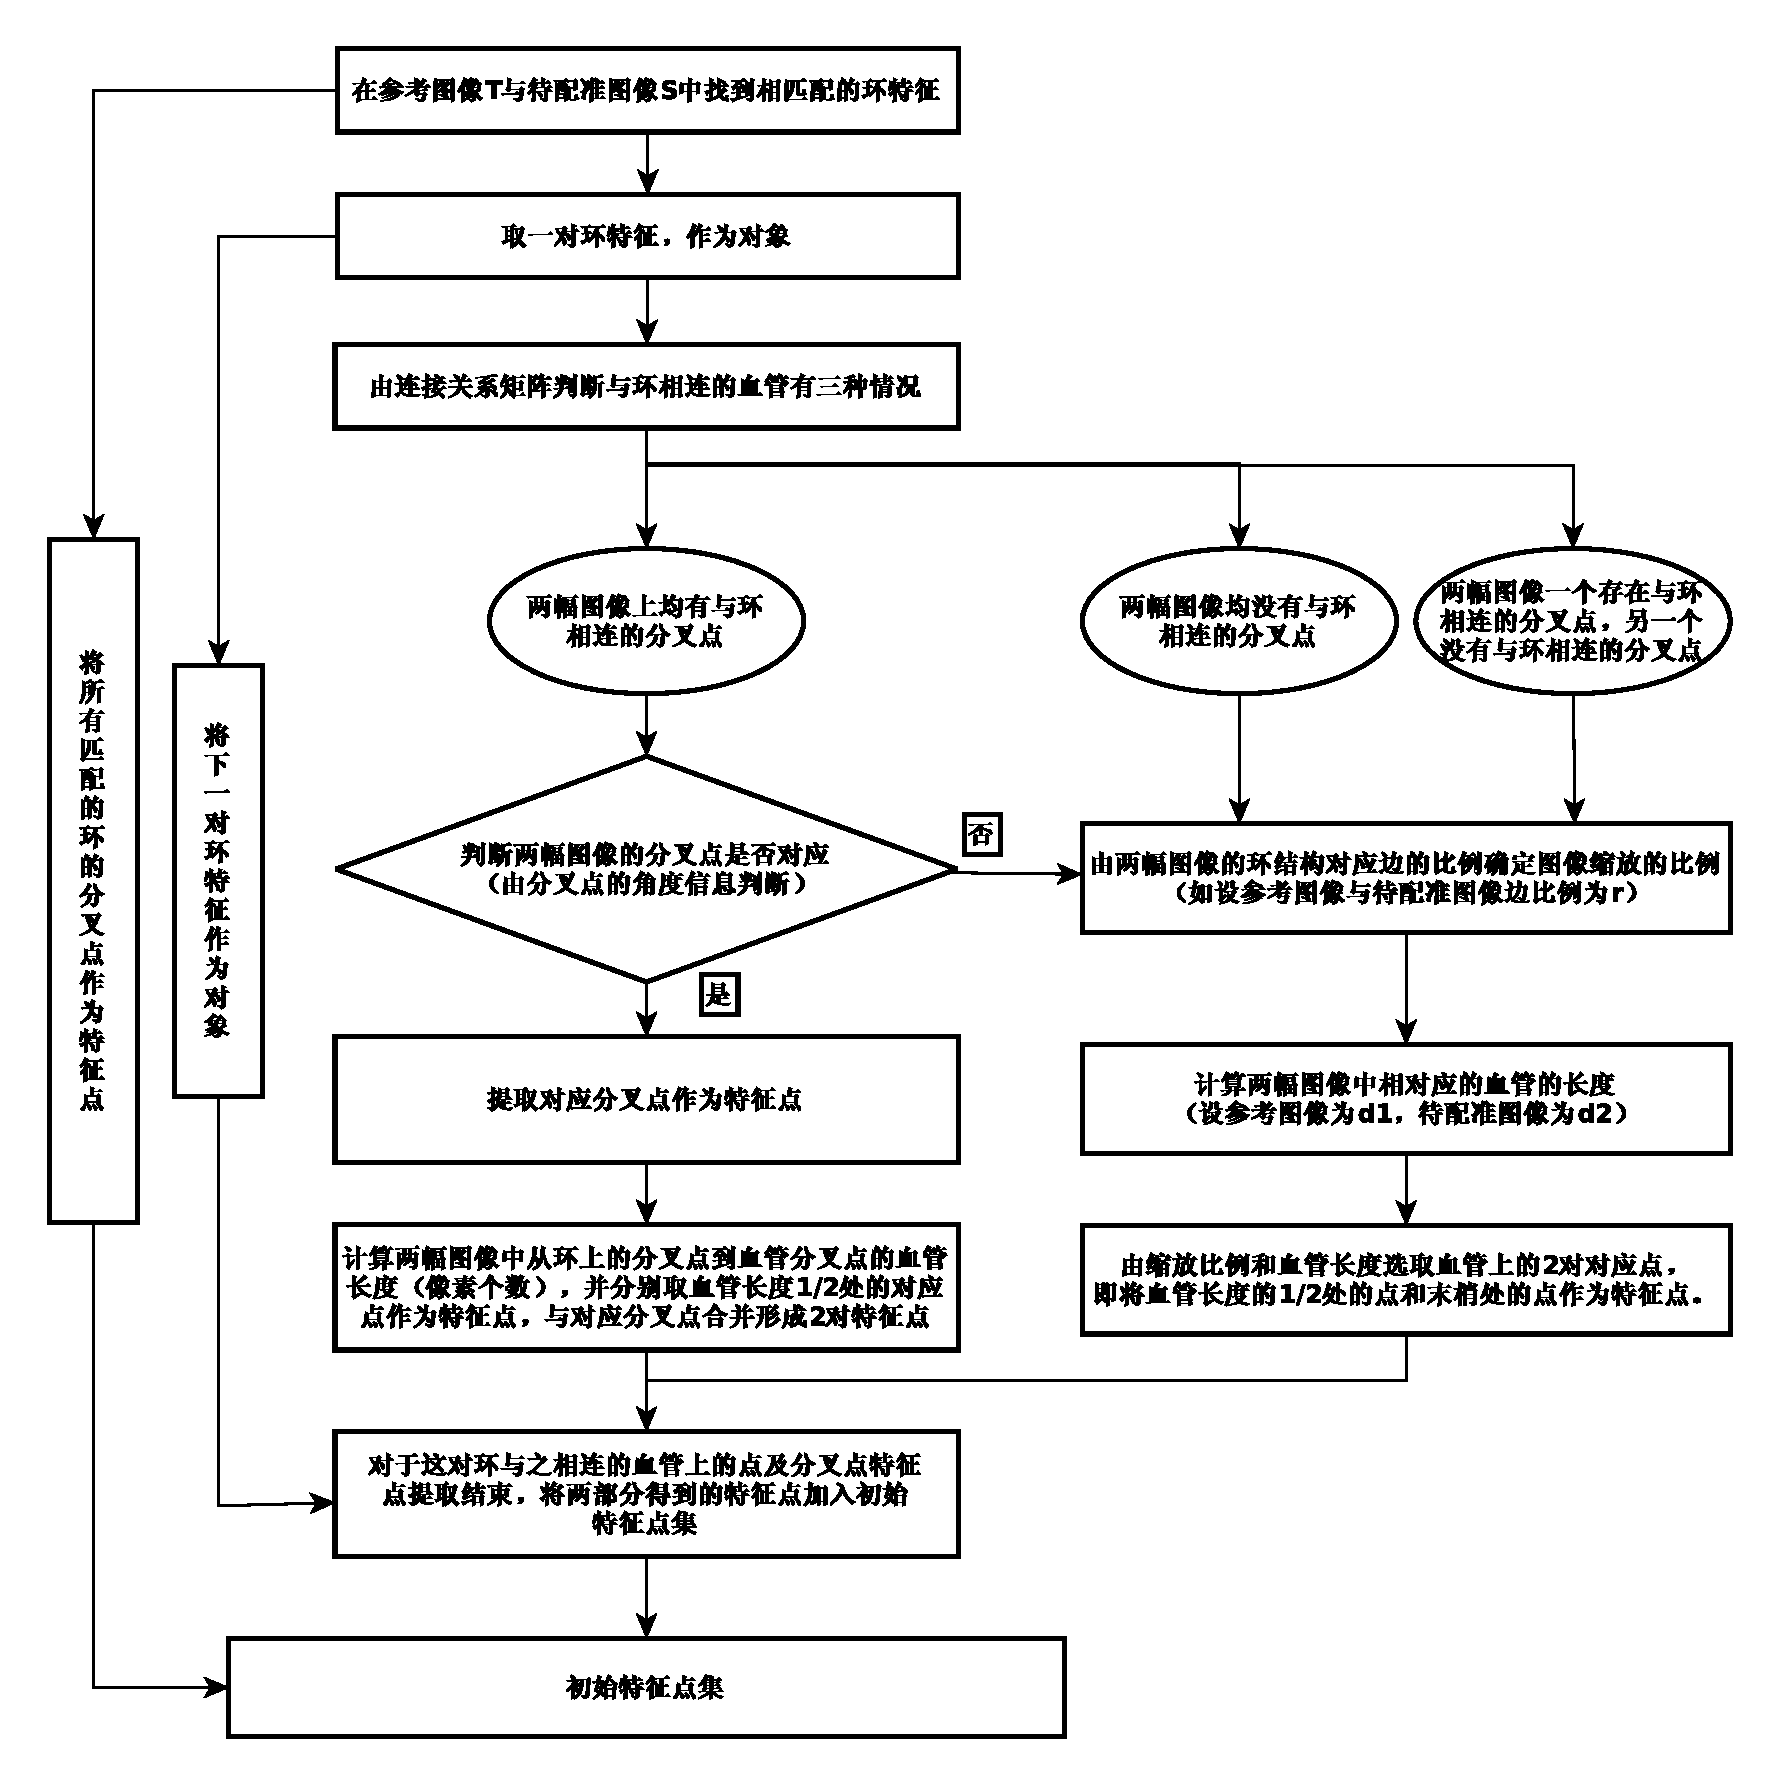
\includegraphics[width=1\textwidth]{chap03/global}
  \caption{将与环相连的血管上的点加入特征点集}
  \label{fig:global}
\end{figure}

步骤为:
\begin{enumerate}
\item 从环上的一个分叉点开始,根据分叉点之间的连接关系,搜索与之相邻的除环以外的其他点。若参考图像与待配准图像上都存在这样的点,则转入第二步,否则转入第三步。
\item 判断这些与分叉点相邻的分叉点是否是相对应的,若是,则取血管的中心点与这个点加入特征点集,否则,则转入第三步。
\item 考虑到参考图像与待配准图像之间有可能有尺度变化,要通过计算相匹配的环结构中边长的比例关系来确定缩放尺度。从而根据缩放尺度找到相对应的与环相连的血管的中心点和端点,加入特征点集。

图\ref{fig:global points}显示了最匹配的环结构及与其相连的血管上的对应点。蓝色点为最匹配的环结构特征点对,红色点为与通过以上步骤得到的环相连的血管点。从图中可以看出,找到的点都是正确匹配的。
\end{enumerate}


\begin{figure}
\centering
  \begin{minipage}[b]{0.48\textwidth} 
      \centering 
      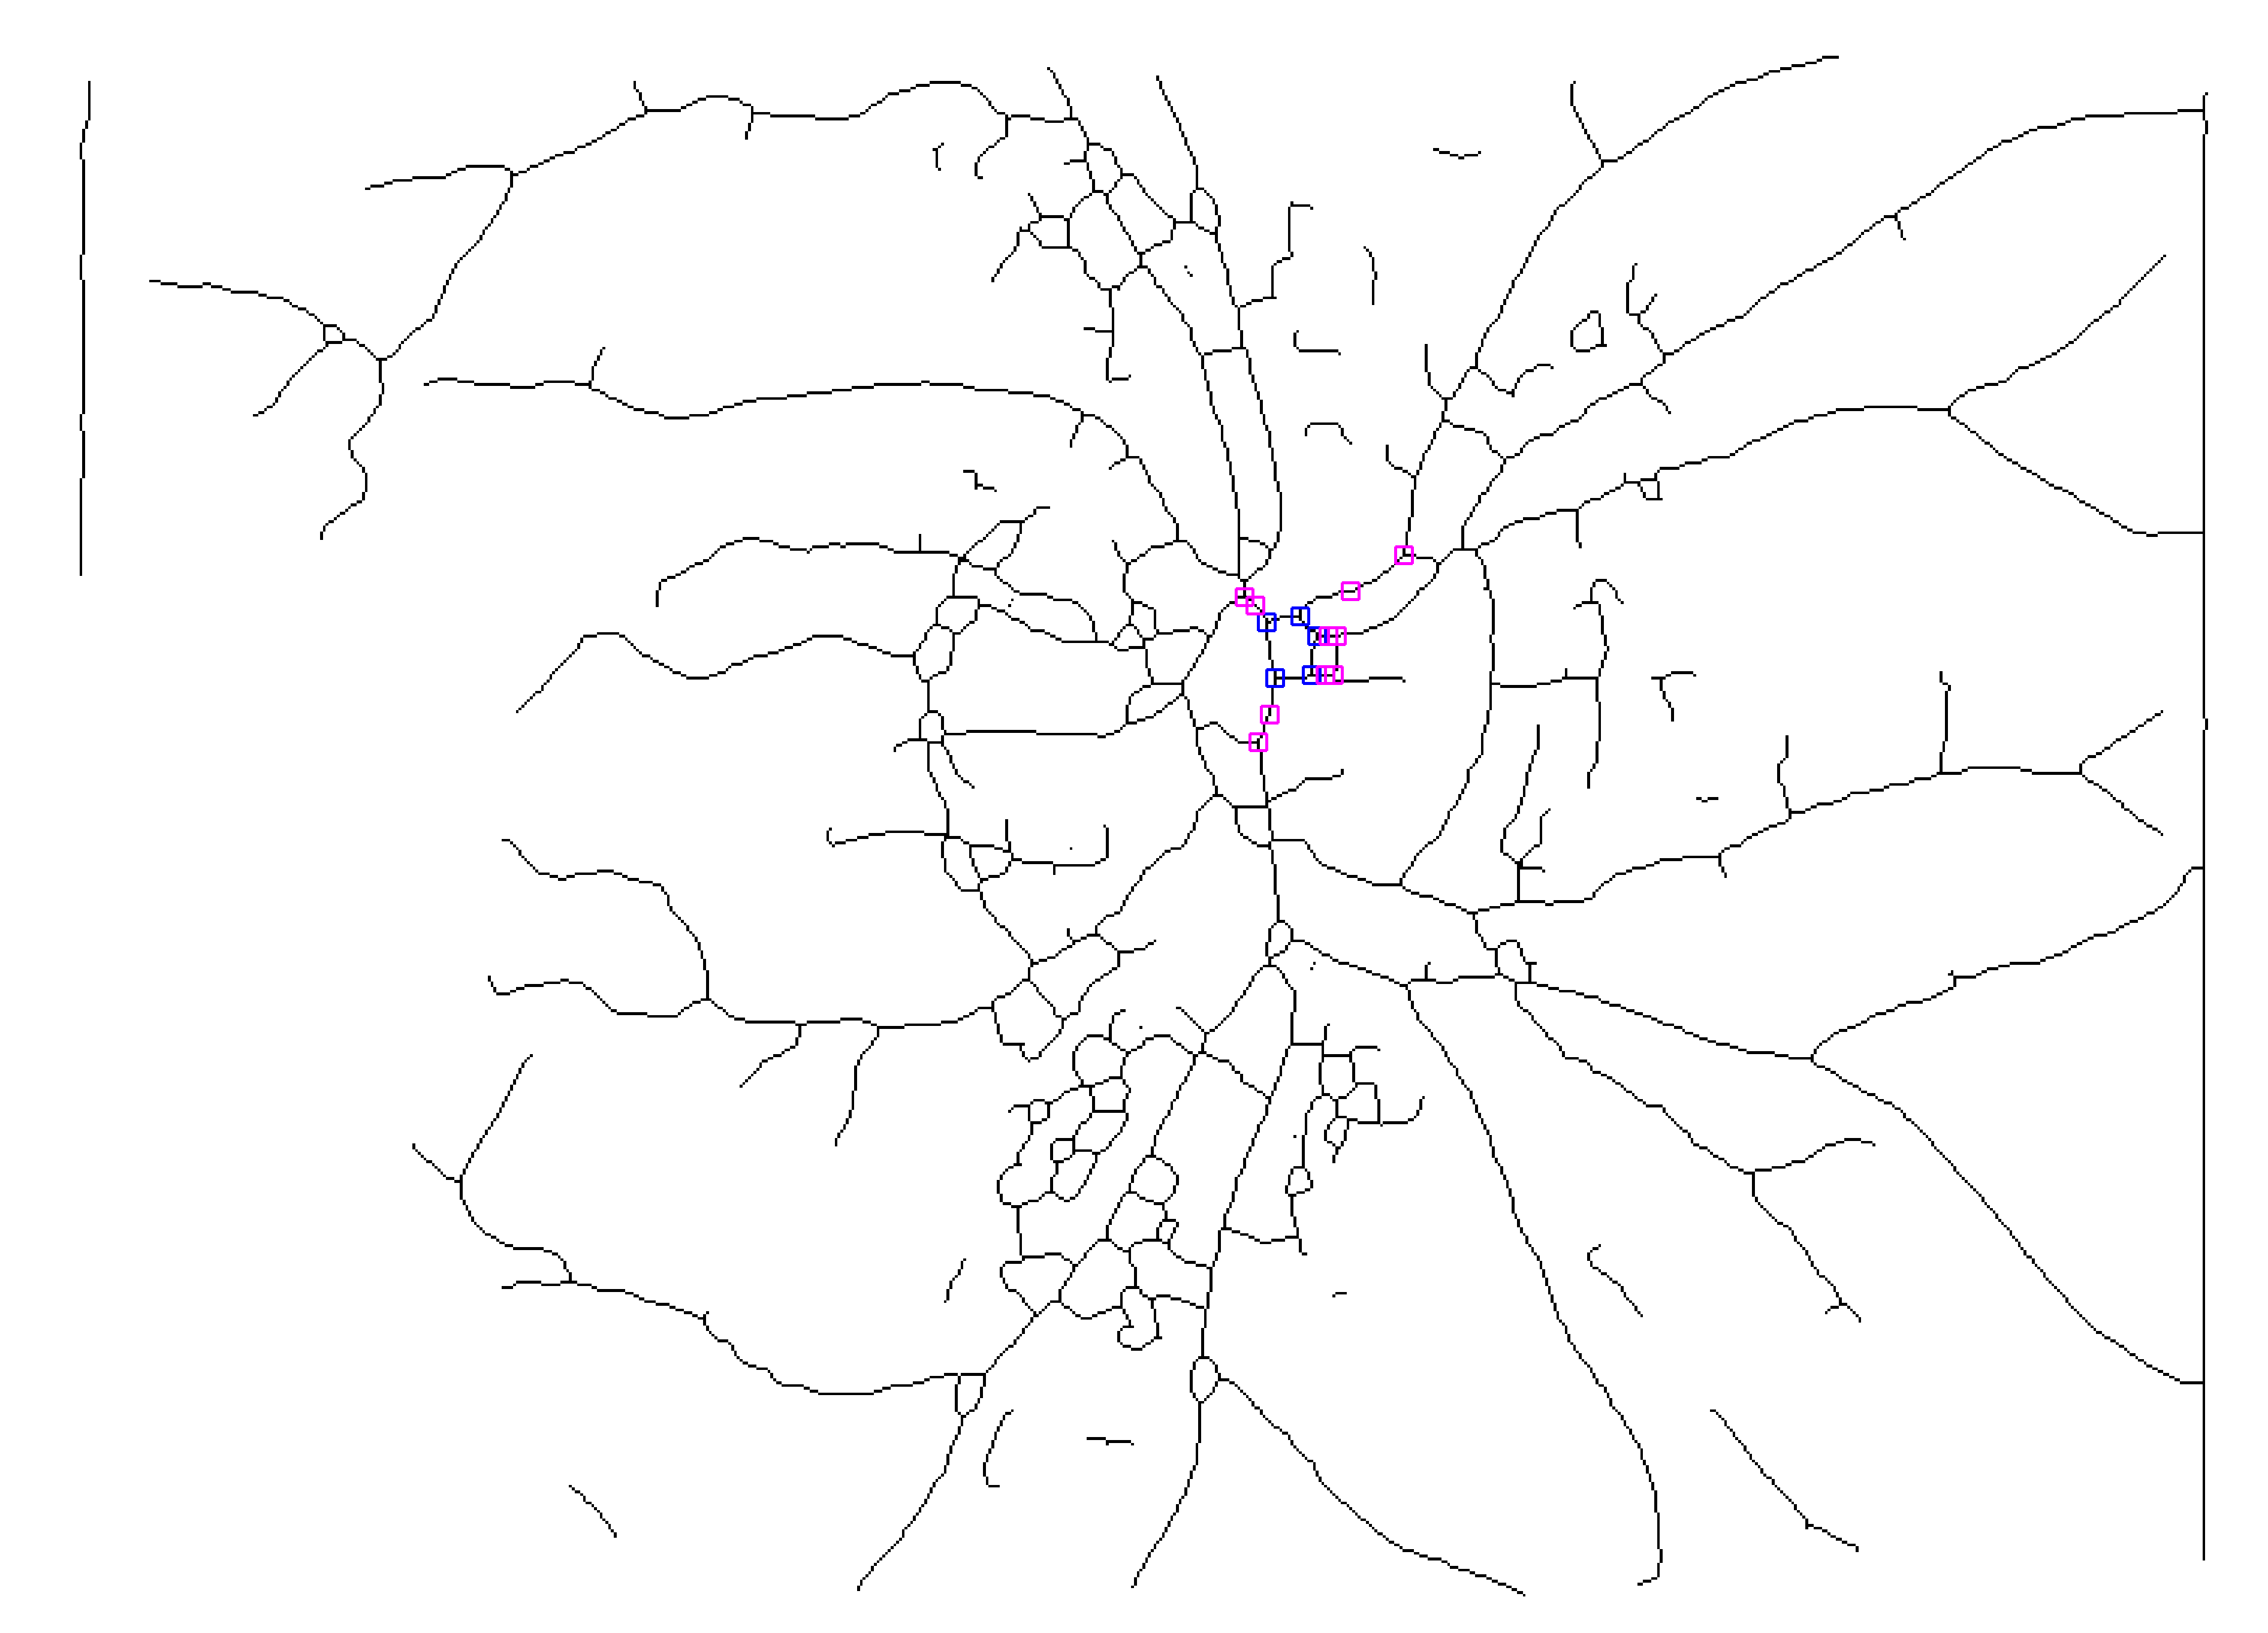
\includegraphics[width=6cm]{chap03/bw1-cycle-vessel}
        \centerline{(a) 参考图像}\medskip
    \end{minipage}
  \begin{minipage}[b]{0.48\textwidth}
    \centering
    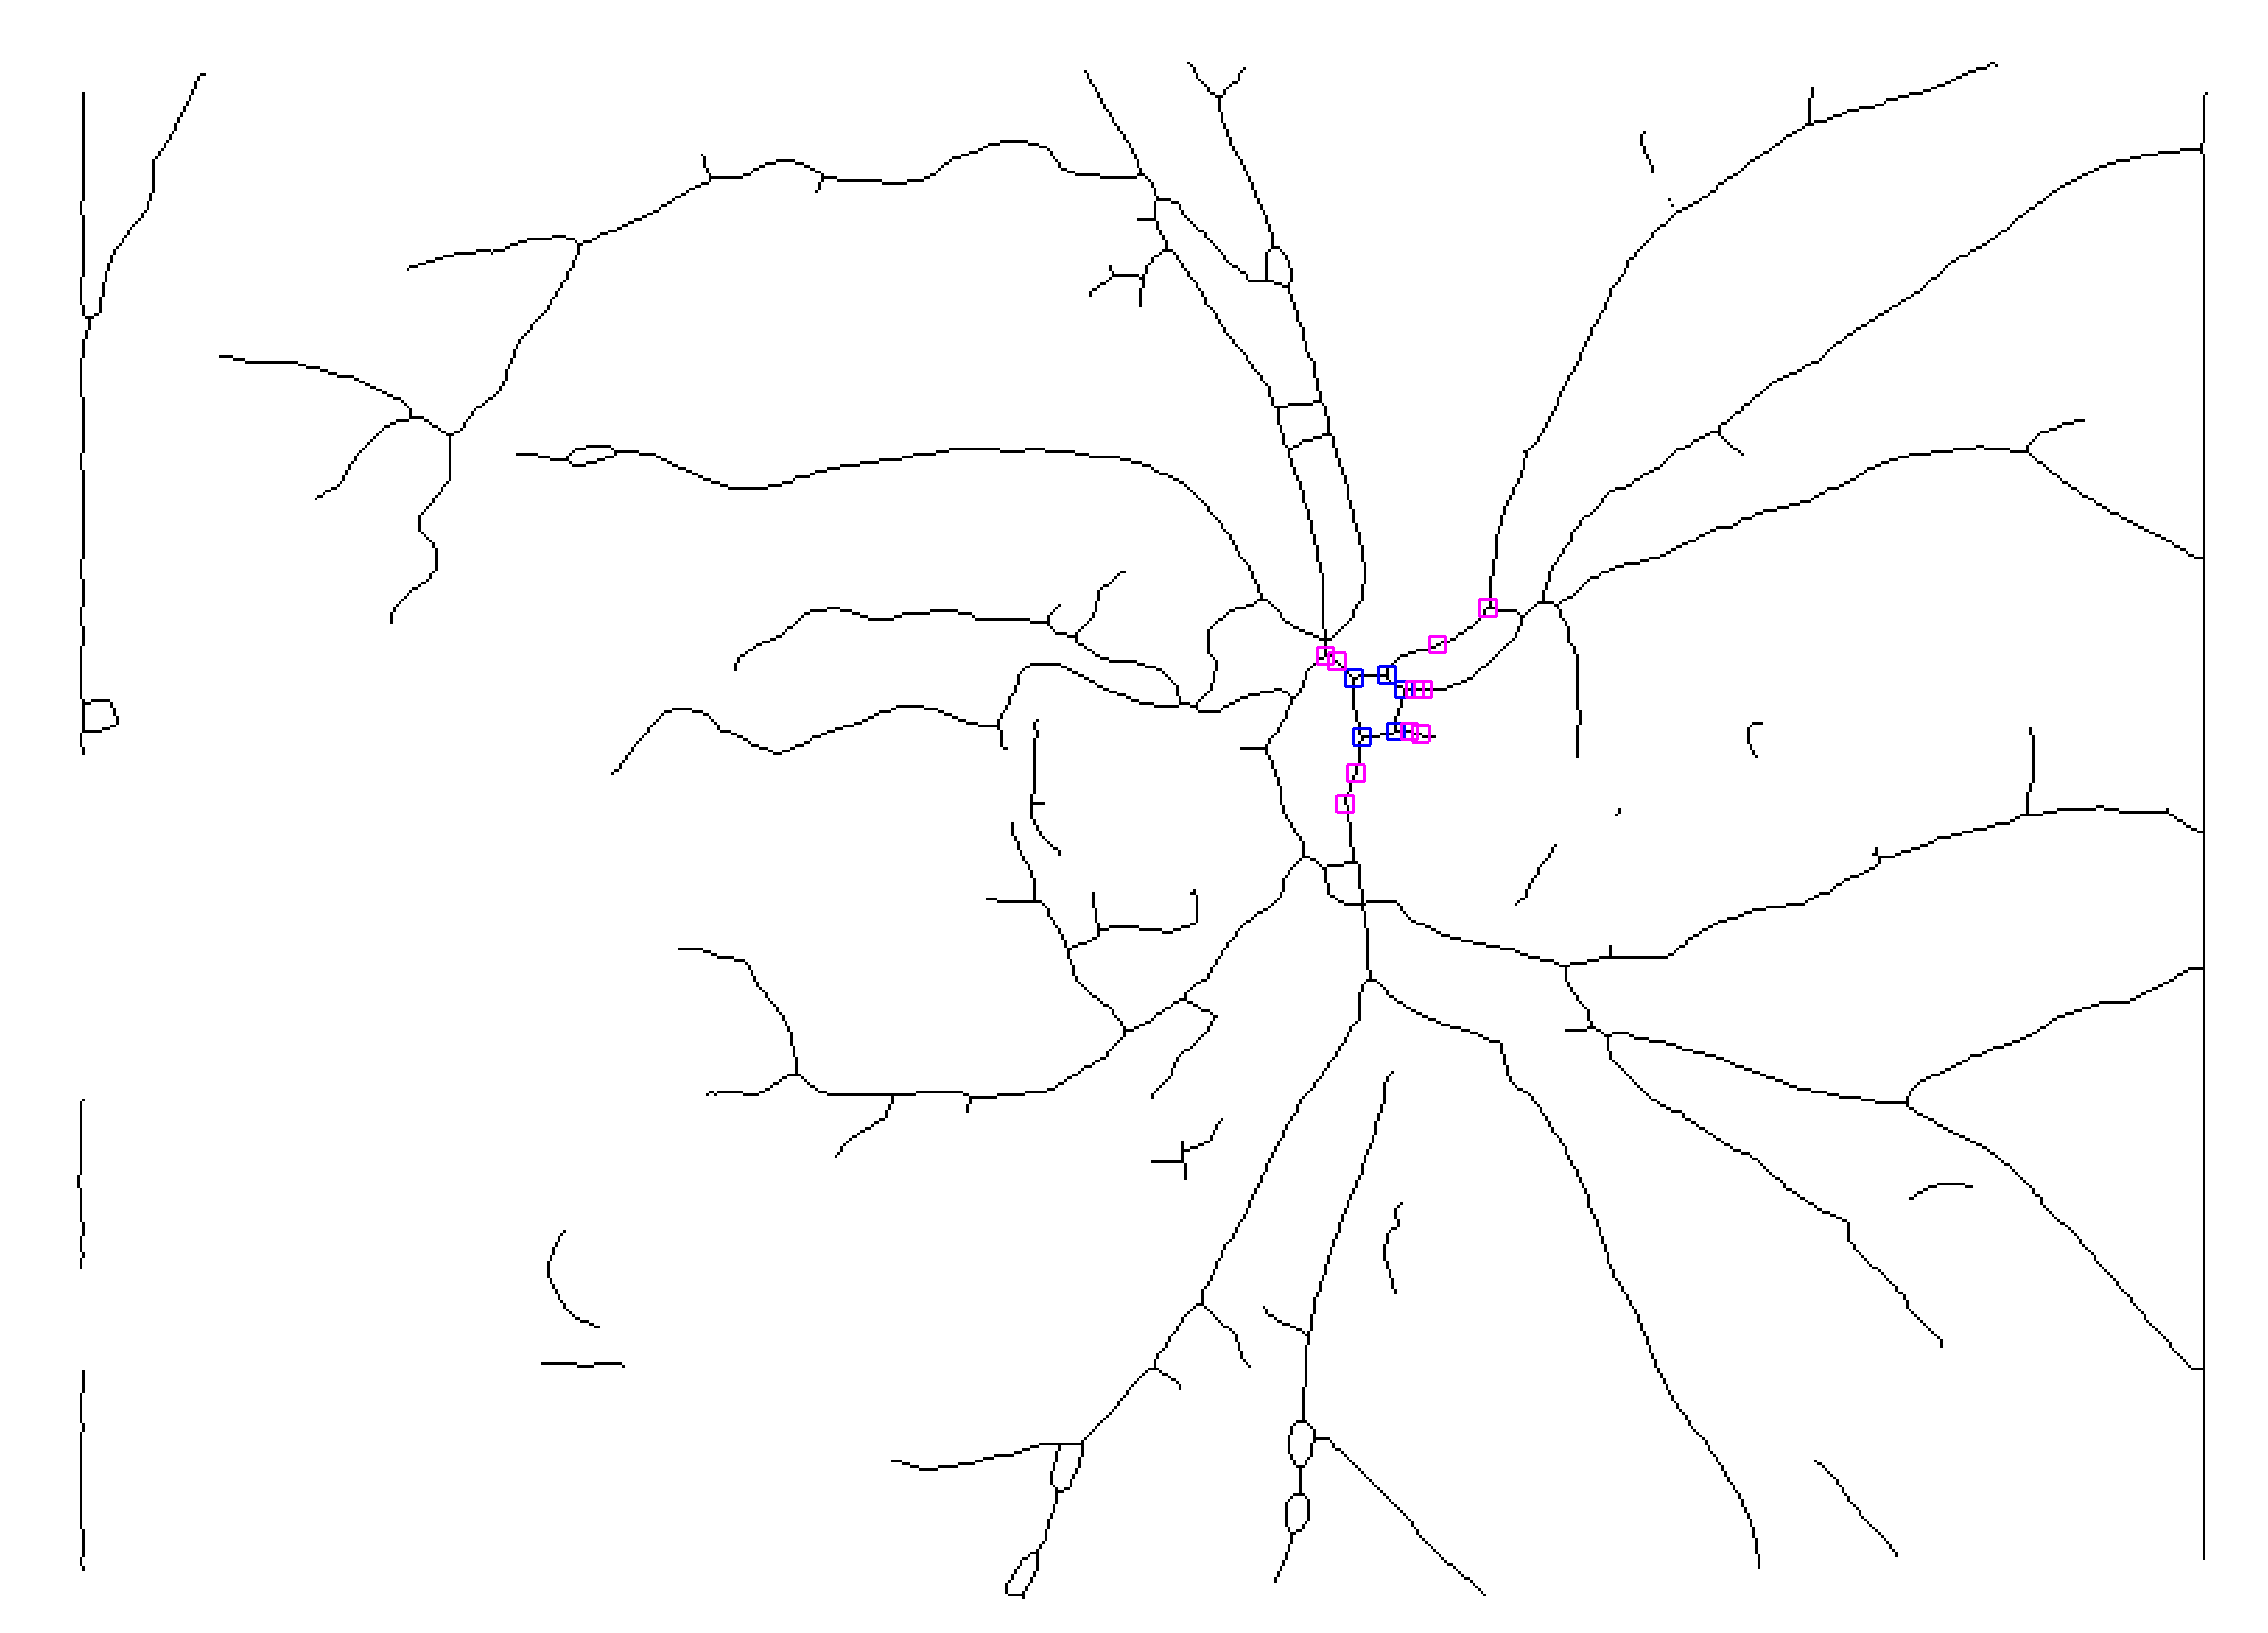
\includegraphics[width=6cm]{chap03/bw2-cycle-vessel}
      \centerline{(b) 待配准图像}\medskip
  \end{minipage}
\caption{相匹配的环结构及与其相连的血管上的对应点}
\label{fig:global points}
\end{figure}


根据特征点集中相对应的特征点的坐标进行相似性变换,于是,得到了全局初始配准结果,如图\ref{fig:global results}。


\begin{figure}
\centering
  \begin{minipage}[b]{0.48\textwidth} 
      \centering 
      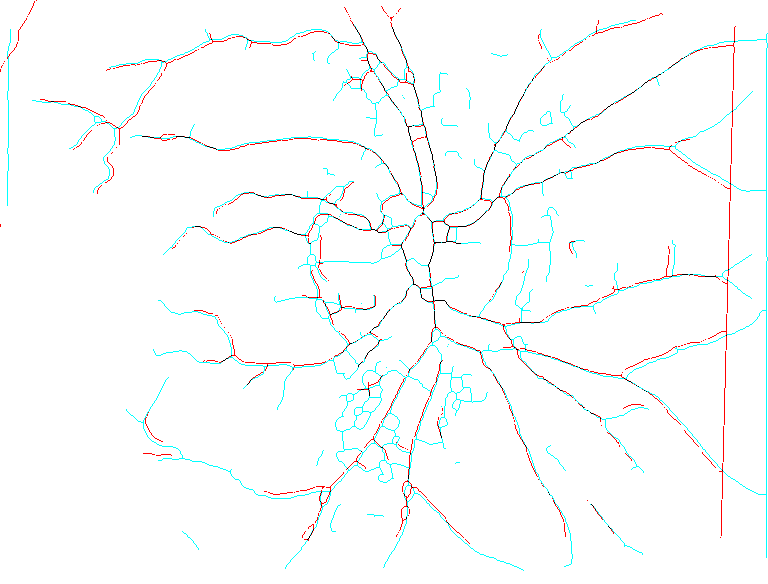
\includegraphics[width=6cm]{chap03/067-119-initial_reg}
        \centerline{(a) 骨架化配准结果}\medskip
    \end{minipage}
  \begin{minipage}[b]{0.48\textwidth}
    \centering
    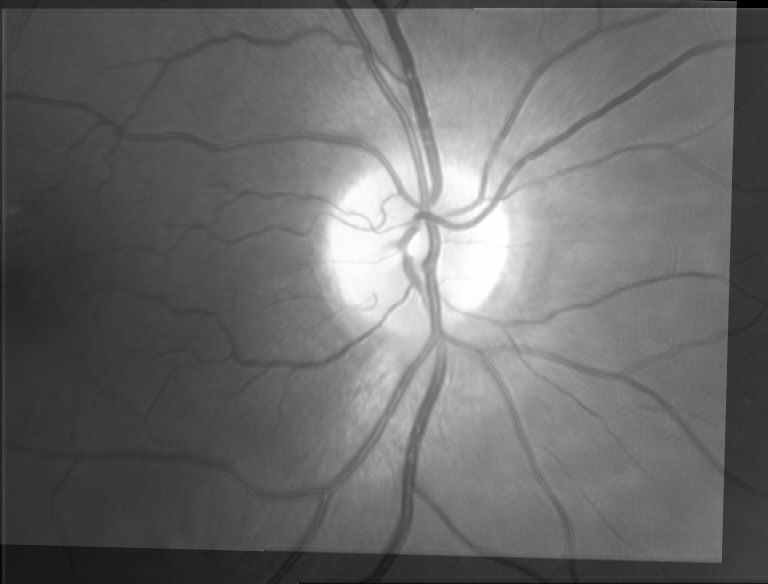
\includegraphics[width=6cm]{chap03/067-119-initial_result}
      \centerline{(b) 配准后的原图像}\medskip
  \end{minipage}
\caption{全局初始配准结果}
\label{fig:global results}
\end{figure}




由图\ref{fig:global results}可以看到,虽然使用环上的分叉点及与环相连的血管上的点能准确的进行配准,但仍不够鲁棒,远离这些特征点的区域会出现几个像素的偏差。因此,我们采用了一种从全局到局部的策略,即增加一些局部分叉点来纠正配不准的区域,以此来提高配准精度。配准流程图如图\ref{fig:local}。基本步骤为:
\begin{enumerate}
\item 检测参考图像中的所有分叉点,并分别以这些分叉点为中心,形成$5 \times 5$像素的区域。
\item 分别在配准后的图像中这些小区域内检测分叉点。根据分叉点的角度信息判断是否有与待配准图像中的分叉点相对应的分叉点。若有,则计算这两个分叉点之间的欧式距离。若欧式距离大于3,我们认为这一对对应点是没有配准的,那么应将其加入新的特征点集。否则,则认为没有未配准的对应点对。
\item 根据初始配准时相似性度量参数及对应点的坐标,将特征点集中配准后的图像中的分叉点映射回待配准图像中,将新的特征点集中的点变为参考图像与待配准图像中相对应的分叉点。
\item 将新的特征点集与初始特征点集合并,形成最终的特征点集。重新采用相似性变换进行第二次配准,得到经过局部修正的最终的配准结果。
\end{enumerate}
图\ref{fig:final-results}给出了两个例子,显示了全局与局部配准结果。从图中我们可以看出,在全局初始配准中未配准的血管经过局部配准后得到了纠正。
\begin{figure}[!ht]
  \centering
  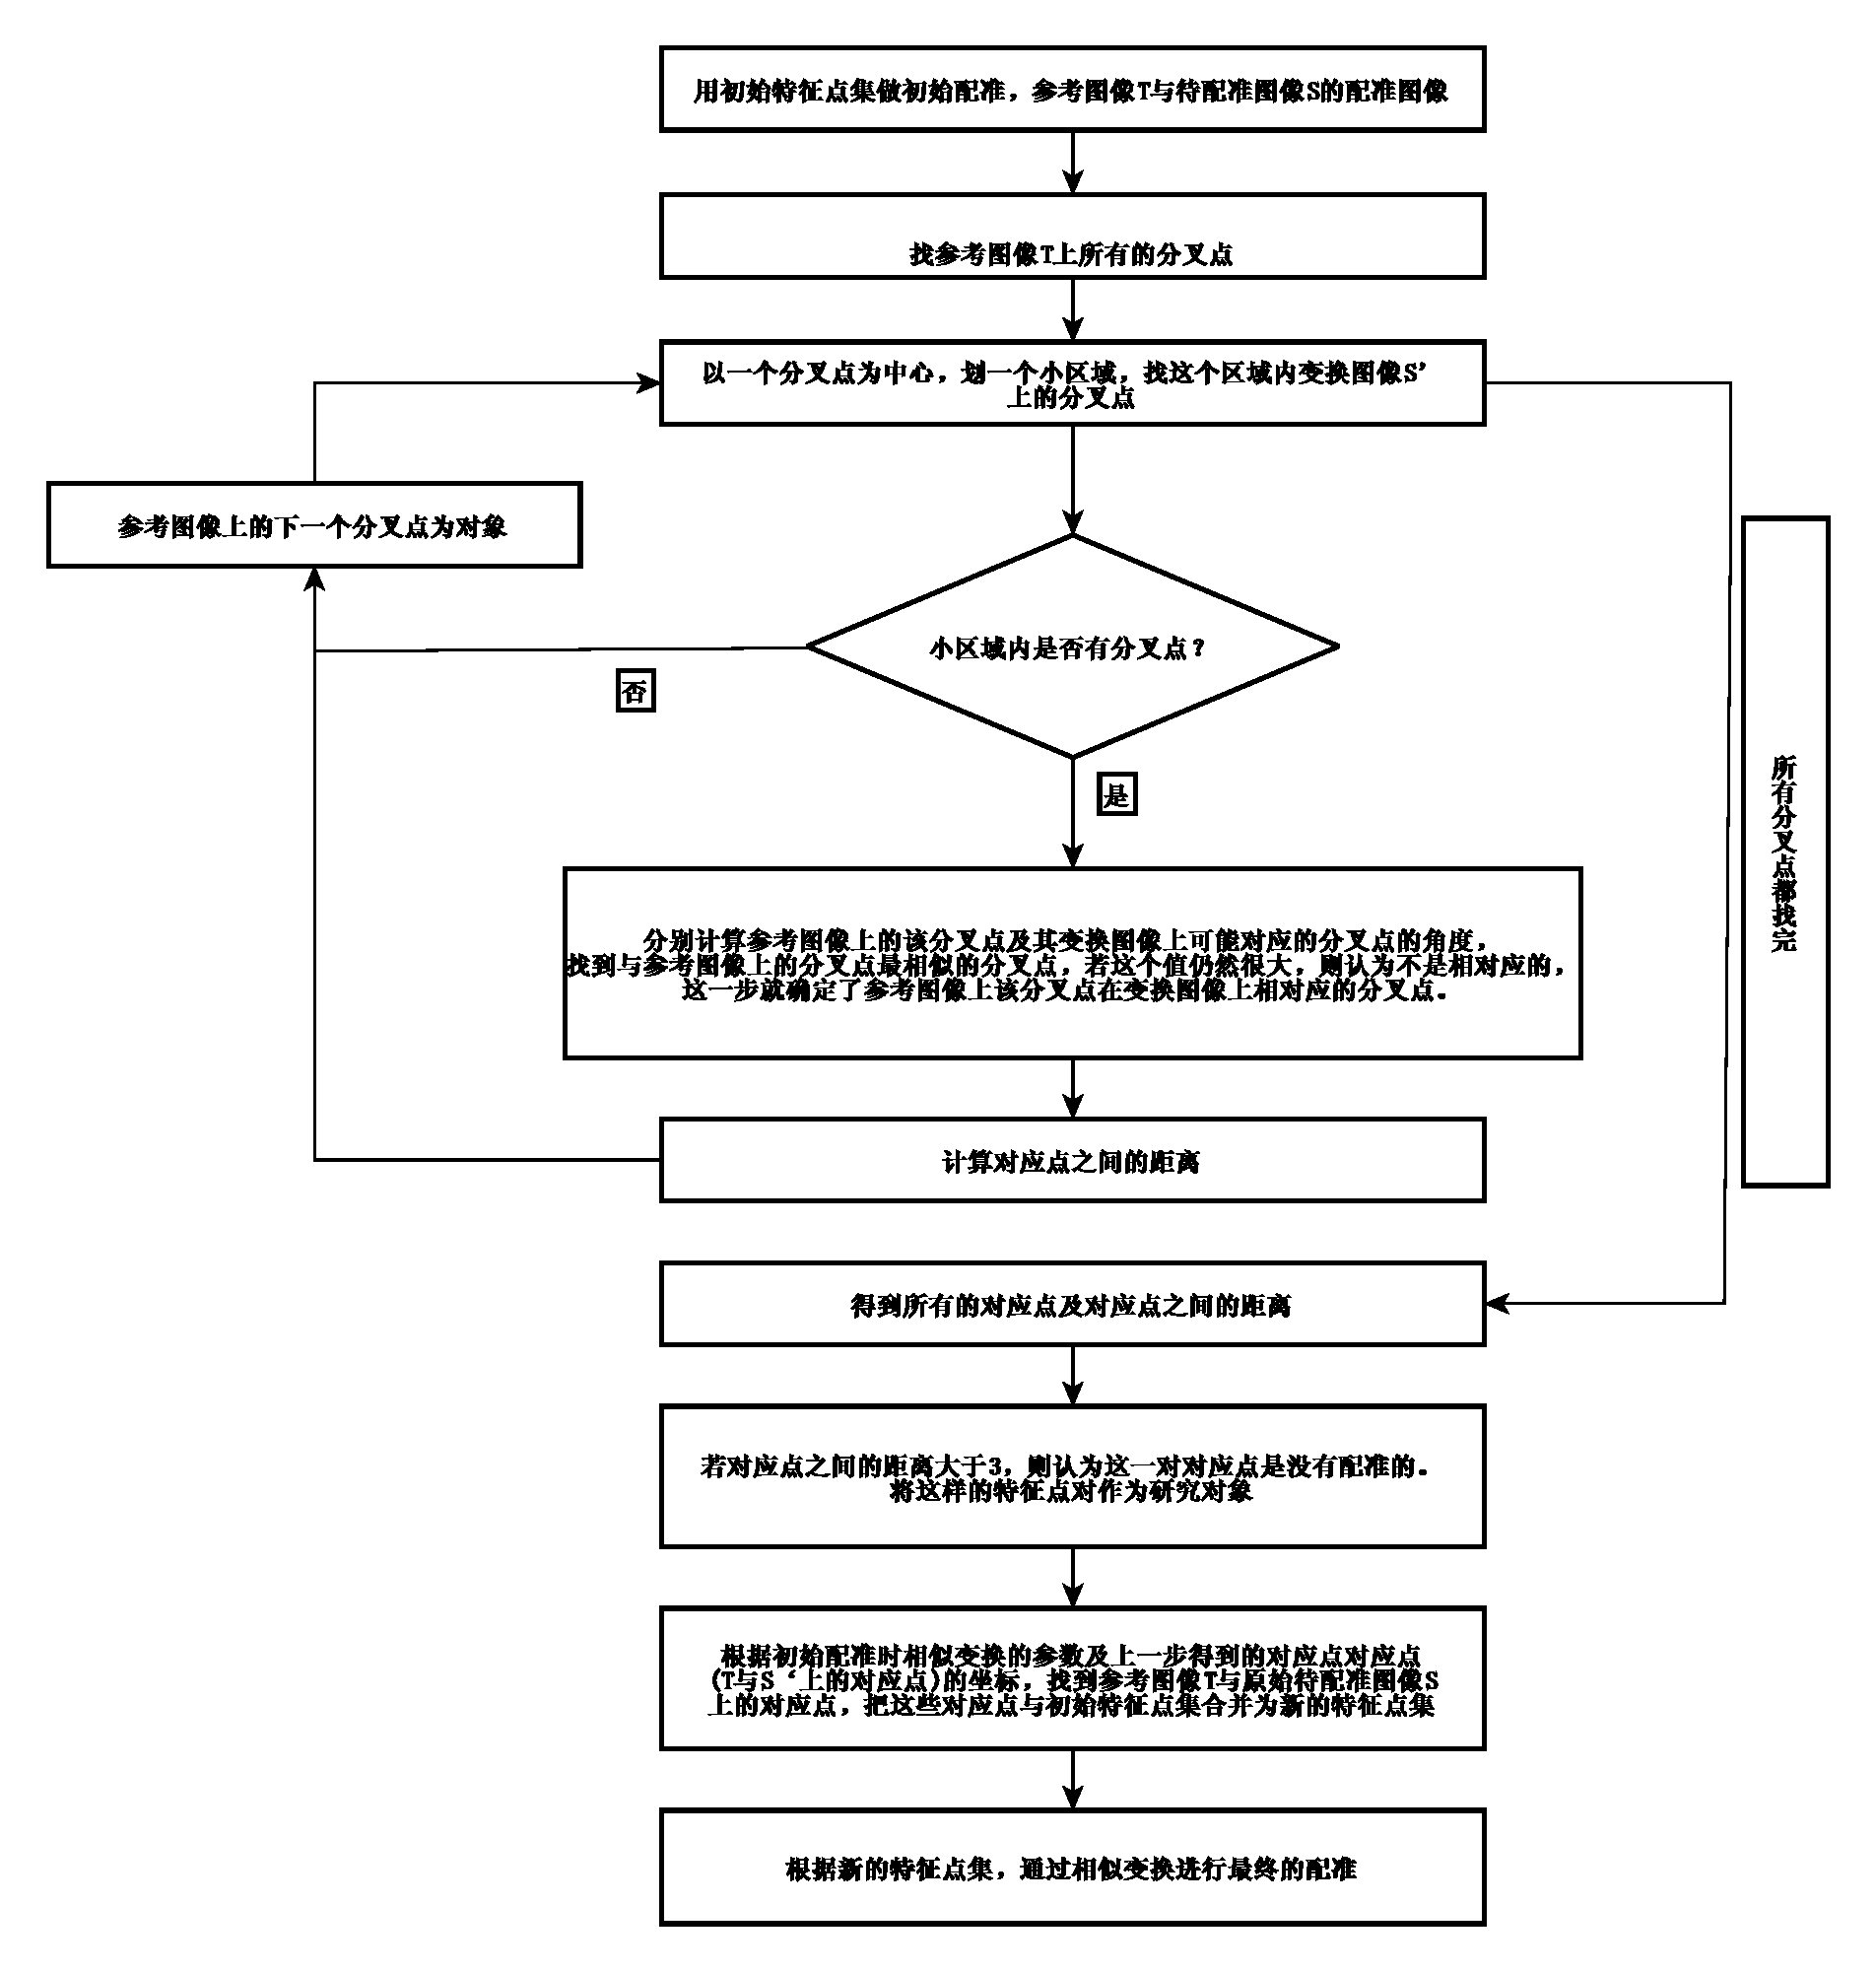
\includegraphics[width=1\textwidth]{chap03/local}
  \caption{局部配准流程图}
  \label{fig:local}
\end{figure}

\begin{figure}[!ht]
\centering

\begin{minipage}[b]{0.3\textwidth} 
      \centering 
      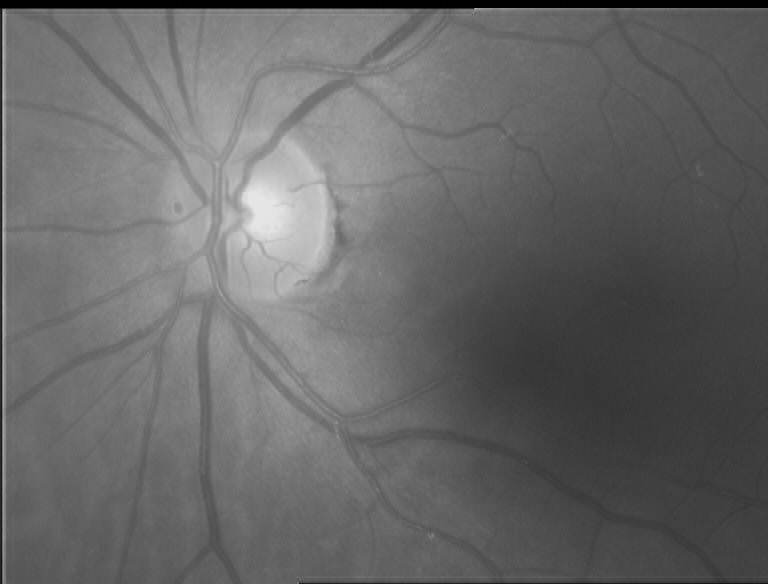
\includegraphics[width=4cm]{chap03/R160.png}
        \centerline{(a) 参考图像}\medskip
\end{minipage}
  \begin{minipage}[b]{0.3\textwidth}
    \centering
    \includegraphics[width=4cm]{chap03/R161.png}
      \centerline{(b) 待配准图像}\medskip
  \end{minipage}
\begin{minipage}[b]{0.3\textwidth}
	\centering
      \includegraphics[width=4cm]{chap03/160-161-result.png}
        \centerline{(c) 配准后的原图像}\medskip
    \end{minipage}
\\
  \begin{minipage}[b]{0.48\textwidth}
    \centering
    \includegraphics[width=5cm]{chap03/160-161-initial.png}
      \centerline{(d) 全局配准骨架化结果}\medskip
  \end{minipage}
 \begin{minipage}[b]{0.48\textwidth}
    \centering
      \includegraphics[width=5cm]{chap03/160-161-local.png}
        \centerline{(e) 局部配准骨架化结果}\medskip
    \end{minipage}
\\
  \begin{minipage}[b]{0.3\textwidth}
    \centering
    \includegraphics[width=4cm]{chap03/R096.png}
      \centerline{(f) 参考图像}\medskip
  \end{minipage}
\begin{minipage}[b]{0.3\textwidth}
      \includegraphics[width=4cm]{chap03/R212.png}
       \centerline{(g) 待配准图像}\medskip
    \end{minipage}
  \begin{minipage}[b]{0.3\textwidth}
    \centering
    \includegraphics[width=4cm]{chap03/096-212-result.png}
          \centerline{(h) 配准后的原图像}\medskip
  \end{minipage}
\\
 \begin{minipage}[b]{0.48\textwidth}
    \centering
      \includegraphics[width=5cm]{chap03/096-212-initial.png}
       \centerline{(i) 全局配准骨架化结果}\medskip
    \end{minipage}
  \begin{minipage}[b]{0.48\textwidth}
    \centering
    \includegraphics[width=5cm]{chap03/096-212-local.png}
           \centerline{(j) 局部配准骨架化结果}\medskip
  \end{minipage}
\caption{全局与局部配准结果}
\label{fig:final-results}
\end{figure}
\section{骨架化对准精度}

无论是对特定的图像、所使用的配准方法还是应用领域,都需要一个准确的评估方法来估计配准结果的准确性与精确性。精度评价是一个重要的问题,因为错误可能出现在配准过程的各个阶段有时很难区分配准错误和实际图像内容的差异。用人眼观察配准结果并不是一种十分科学的方法,因为存在一些主观因素来影响评估的准确性,通过定量的评价,可以得到对配准结果的准确估计。本节,我们介绍了几种基本的错误类型和评估方法\cite{barbara}并提出了我们自己的骨架化对准精度方法。


\begin{enumerate}
\item 定位误差。由于特征检测的不准确性引起的位移叫做定位误差。大多数特征检测的平均精度是真实的数据与计算机模拟的数据之间的比较,也可用于估计在特定情况下的定位误差。通过选择最优的特征检测算法,定位误差可能会减小,但在检测到的特征数量与平均定位误差之间通常有一个权衡。有时,我们更倾向于选择更多的特征和稍高的定位误差。

\item 匹配误差。匹配误差是在建立特征之间的对应关系时,错误匹配的特征数量。匹配误差是一个严重的问题,因为由于特征匹配错误,在用这对错误匹配的错误进行变换模型估计时,估计的变换参数是不准确的,因此通常会导致配准的失败。所以在进行特征匹配时应该尽量避免这个问题。幸运的是,在大多数情况下,匹配误差可以通过鲁棒性的匹配算法来避免。在两个不同的匹配方法应用于同一个特征集时,错误匹配可以通过一致性检验来发现。当两种方法都能找到的特征对为有效的特征对,其他的特征对需要做进一步的处理。若没有其他可靠的匹配方法,可以通过交叉验证的方式来消除错误的匹配。在每一步中,在特征集中排除一对特征并计算映射参数,然后观察通过这个模型,这对被排除的特征对的映射结果如何。若变换后与变换前的位移变化比较小,在某一阈值以下,则认为是有效的特征对。

\item 对准误差。对准误差为用于做配准的映射模型与实际的图像间的几何变形之间的差异。在实际应用中,对准误差是不可避免的。变换参数的计算可能不精确,导致所选择的映射模型可能与实际的变换模型的参数是不相对应的。

\end{enumerate}


然而,对准误差的计算是一项艰巨的任务,尤其对于生物医学应用,更加难以定量评估。因为缺乏标定好配准后的真实数据(Ground Truth),因此得到的配准后的图像不能与标定好的真实数据进行比较以得到估计结果。目前,有几种常用的评估方法,第一种方法是使用标记的位置信息,第二种是通过评估血管中心线的平均距离,第三种通过互信息\cite{kolar}。

\begin{enumerate}
\item 通过评估标记的位置,而已量化配准的精确性。配准前后的相应标记错误(ECL)的计算公式为:
\begin{align}
ECL^i = Median_{j}||p_j^i - T(q_j^i)|| 
\end{align}
其中,$p_j^i$和$q_j^i$是第i幅图像中的两个匹配的标记,T是最终的几何形变。中值对于标记对应的可能错误更具有鲁棒性。图像集的平均标记错误误差为每幅图像中值的平均值:
\begin{align}
E_1 = Mean_i(ECL^i)
\end{align}
\item 血管距离。血管距离准则值得是血管树中心线的平均距离。参考图像与待配准图像需进行分割及骨架化处理以得到血管中心线。但由于不同的图像的光照变化不同,分割结果也不同,为了克服这个问题,这种评价方法采用两幅图像的所有血管中心线点的中值距离作为标准。这对在分割中存在差异的情况具有鲁棒性。一对图像的中心线错误估计(CEM)可以定义为:
\begin{align}
CEM^i  = Median_j||p_j^i - T(q_j^i)||
\end{align}
其中,$p_j^i$和$q_j^i$是两对匹配的血管点,T是最终的几何形变。每对图像的中值都被计算后,求均值以得到数据集的最终配准估计:
\begin{align}
E_2 = Mean_i(CEM^i)
\end{align}
但CEM值取决于图像的分辨率。
\item 互信息可以作为配准结果的一个评估标准。归一化的互信息(NMI)可以通过计算图像重合区域来获得:
\begin{align}
NMI(A, B) = \frac{H(A)+H(B)}{H(A, B)}
\end{align}
$H(A), H(B)$和$H(A,B)$分别是边缘和联合熵。采用互信息进行评估的优点是它不依赖于图像的分辨率。
\end{enumerate}



我们采用多尺度分割方法,对于一幅参考图像与一幅待配准图像,分割与骨架化后会产生$14 \times 14$个多尺度结果,并且每一个尺度将产生7种环结构及其组合,故当这两幅图像进行配准时会产生$14 \times 14 \times 7$个配准结果。基于此,我们提出了一种骨架化对准精度用来定量的评估配准结果并且根据这个评估优化选择分割尺度与用来配准的环结构特征。

具体步骤为:
\begin{enumerate}
\item 给定一个参考图像的骨架化结果$M_i (i = 1, 2, \ldots, 14)$,一个待配准图像的骨架化结果$N_j (j = 1, 2, \ldots, 14)$,$N_j$与$M_i$用一种类型的环结构$L_k(k=1, 2, \ldots, 7)$在全局到局部的策略下进行配准,得到配准结果$N_{jMi}$。
\item 对于在$N_{jMi}$中的每个血管点,以这个血管点为中心,在$M_i$中选择一个$7 \times 7$区域,在这个区域中你计算与这个血管点相邻最近的像素的距离d。若在这个区域中没有与这个血管点相邻最近的点,则标记这个血管点无效。
\item 骨架化对准精度被定义为$SAEM_{ijk} = (\sum d) / Num_v$,$Num_v$是在$N_{jMi}$中无效点的数量。
\item 当$Num_v / Num_{N_j} \geq 50 \%$并且$Num_{N_{jMi}} / Num_{N_j} \geq 38 \%$时SAEM有效,$Num_{(.)}$表示在$(.)$中的像素数量。
\end{enumerate}

约束条件的设置是很有必要的,它可以排除一些配准结果偏差很大的情况。因为当两幅图像基本没有配准的情况下,在$7 \times 7$区域内可能检测不到相对应的血管点,这样会使得SAEM的值很小,相对应的图像则被认为是匹配的很精准。约束条件的设置就避免了这种情况的发生。通过骨架化对准精度,最佳的配准结果将会被自动的选择出来,而相对应的尺度和环结构的类型就会知晓。同时,SAEM算法还可以通过配准后两幅图像对应点的距离这个量化值来定量的评判配准结果。整个算法的整体框图如图\ref{fig:framework}。
\section{对比实验}
\label{}
据我们所知,目前没有公开的用来做视网膜配准的数据集。因此我们用VARIA数据集\cite{ortega2009retinal,ortega2009personal}来进行实验来评估我们的方法。VARIA数据集是用来做认证的,这个数据集目前包括从139个个体中获取的233张视网膜图像,其中有59组是从相同个体中拍摄的不同图像。从这59组数据中我们以每两张取自同一个体的不同视网膜图像为对象,共得到153对。这些视网膜图像是通过拓普康免散瞳NW-100相机在$768 \times 584$分辨率下获取的。

针对视网膜图像光照不均匀、中央亮、四周暗、反差过强、对比度弱、有强噪声干扰的特点,我们提出了基于环结构特征的从全局到局部的视网膜图像配准方法。环结构由血管分叉点和交叉点及与它们相连的血管组成。为了克服对视网膜分割结果的依赖性,我们采用多小波核多层分解方法,从而产生多尺度的血管树。不同尺度的血管树所代表的分割的精细程度不同。然后我们提出了基于空间的深度优先搜索算法来提取由多个不同数量的分叉点组成的多环特征,归一化的分支角度和长度来作为特征向量,采用相似性度量来进行全局初次配准。对于远离匹配特征的区域,我们采用局部分叉点信息来纠正配准精度。最后,我们采用骨架化对准精度来优化特征和尺度的选择,实验证明,我们的方法对于视网膜配准来说是有效且可行的。

为了通过实验来说明我们的方法是可行且有效的,我们通过不同变换模型、不同特征、不同方法进行了对比实验,用成功率(SR)及骨架化对准精度(SAEM)来定量的评估这153对图像的实验结果。

\subsection{不同变换模型之间的对比实验}

变换模型对于用来配准的不同特征是十分重要的。变换模型的选择能很大程度上影响配准结果。为了证明相似性变换更加适合环结构特征,我们用相似性变换、仿射变换、二次多项式变换进行了对比实验,表\ref{tab:models}给出了采用不同模型的配准结果。从表中可以看出,虽然多项式变换的SAEM值是最小的,但它对于环结构仍然是不适用的,因为其成功率只有16.99\%,所以不适用于做配准。仿射变换由于在变换过程中要改变环结构中的角度信息,所以配准成功率也相对较低。相似性变换对于我们提出的环结构特征是最适用的,成功率高达96.73\%,且SAEM值也相对较低。
\begin{table}[!ht]
\caption{不同变换模型之间的对比实验}
\centering
\begin{tabular}{lcc}
\toprule
变换模型 & SR  & SAEM (像素)\\
\midrule
相似性变换 & $\mathbf{96.73\%}$ & $\mathbf{0.938}$ \\
仿射变换 & $50.33\%$ & $1.010$              \\
二次多项式变换 & $16.99\%$ & $0.231$\\
\bottomrule
\end{tabular}
\label{tab:models}
\end{table}

图\ref{fig:transform-fig}给出了两组对比实验图,从图中可以看到相似性变换成功配准且配准精度较高,仿射变换基本配准,但有几个像素的距离,而多项式变换配准失败。
\begin{figure}[!ht]
\centering

\begin{minipage}[b]{0.48\textwidth} 
      \centering 
      \includegraphics[width=6cm]{chap03/similarity1.png}
        \centerline{(a) 相似性变换}\medskip
\end{minipage}
  \begin{minipage}[b]{0.48\textwidth}
    \centering
    \includegraphics[width=6cm]{chap03/similarity2.png}
      \centerline{(d) 相似性变换变换}\medskip
  \end{minipage}
\\
  \begin{minipage}[b]{0.48\textwidth}
    \centering
    \includegraphics[width=6cm]{chap03/affine1.png}
      \centerline{(b) 仿射变换}\medskip
  \end{minipage}
 \begin{minipage}[b]{0.48\textwidth}
    \centering
      \includegraphics[width=6cm]{chap03/affine2.png}
        \centerline{(e) 仿射变换}\medskip
    \end{minipage}
\\
\begin{minipage}[b]{0.48\textwidth}
	\centering
      \includegraphics[width=6cm]{chap03/polynomial1.png}
        \centerline{(c) 二次多项式变换}\medskip
    \end{minipage}
  \begin{minipage}[b]{0.48\textwidth}
    \centering
    \includegraphics[width=6cm]{chap03/polynomial2.png}
      \centerline{(f) 二次多项式变换}\medskip
  \end{minipage}
\caption{不同变换模型的配准结果}
\label{fig:transform-fig}
\end{figure}

\subsection{不同特征之间的对比实验}

表\ref{tab:features}列出了采用不同特征的配准结果,即只用环上的点,环上的点及与环相连的血管上的点,环上的点、与环相连的血管上的点及局部分叉点三种情况。从表中我们可以明显看出,我们采用的从全局到局部的策略,即环+血管+分叉点的特征对配准来说更加鲁棒和准确,使得配准结果具有更高的准确率与最小的SAEM。

\begin{table}[!ht]
\caption{不同特征之间的对比实验}
\centering
\begin{tabular}{p{3.6cm}cc}
\toprule
特征 & SR  & SAEM (pixel)\\
\midrule
环 & $96.73\%$ & $0.938$\\
环 + 血管  & $97.39\%$ & $0.903$\\
环 + 血管 + 分叉点 & $\mathbf{100\%}$ & $\mathbf{0.879}$ \\
\bottomrule
\end{tabular}
\label{tab:features}
\end{table}

为了说明环结构更加适用于视网膜图像配准,我们也采用了Harrias角点检测算法与SIFT算法进行了特征提取,如图\ref{fig:ComparisionFeature}。Harrias角点检测算法检测到的特征点不能与实际观察的视网膜血管特征十分贴合,而且十分杂乱,很难找到对应关系,SIFT算法得到的匹配结果,匹配的特征点基本都是背景点而不是血管点,而且容易出现匹配错误。采用我们的算法,得到两对最匹配的环结构特征对,如图\ref{fig:ComparisionFeature}标记的红色及蓝色点。

\begin{figure}[!ht]
\centering
\begin{minipage}[b]{0.48\textwidth} 
      \centering 
      \includegraphics[width=7cm]{chap03/harrias1}
        \centerline{(a) 参考图像Harrias角点提取}\medskip
\end{minipage}
  \begin{minipage}[b]{0.48\textwidth}
    \centering
    \includegraphics[width=8.5cm]{chap03/harrias2}
      \centerline{(b) 待配准图像Harrias角点提取}\medskip
  \end{minipage}
\begin{minipage}[b]{1\textwidth}
	\centering
      \includegraphics[width=15cm]{chap03/sift}
        \centerline{(c) SIFT特征匹配}\medskip
    \end{minipage}
\\
  \begin{minipage}[b]{0.48\textwidth}
    \centering
    \includegraphics[width=7cm]{chap03/1}
      \centerline{(d) 参考图像中的环结构特征}\medskip
  \end{minipage}
 \begin{minipage}[b]{0.48\textwidth}
    \centering
      \includegraphics[width=8cm]{chap03/2}
        \centerline{(e) 待配准图像中的环结构特征}\medskip
    \end{minipage}
\caption{不同特征的配准结果}
\label{fig:ComparisionFeature}
\end{figure}


\subsection{不同方法之间的对比实验}

2011年,Chen\cite{chen2011retinal,chen2015retinal}等人结合视网膜图像的特点,提出了基于分叉结构的配准方法,分叉结构由一个主分叉点和与它相连的三个相邻分叉点组成,归一化的分支角度和长度作为特征向量,如图\ref{fig:bifurcation structure}。

\begin{figure}[!ht]
  \centering
  \includegraphics[width=0.4\textwidth]{chap03/bifurcation-structure}
  \caption{分叉结构特征}
  \label{fig:bifurcation structure}
\end{figure}

2013年,Shen\cite{shen2012blood}等人扩展了基于分叉结构的配准方法,利用局部的精细配准来纠正配准精度。其局部配准的主要步骤是:
\begin{enumerate}
\item 分别在参考图像和变换后图像上检测分叉点并进行坐标比对,利用界定盒原理找到未匹配上的分叉点。
\item 在参考图像上以任一分叉点q为中心,划定一个$M / p \times N / P$大小的区域,其中P是一个固定值,$M \times N$为图像大小,假如在这个区域内有K个分叉点未匹配上,则说明这个区域的配准精度不高,需要再次进行局部配准。
\item 在未精准配准区域中与参考图像中找到一组对应的分叉结构,得到组成分叉结构的分叉点的坐标。这对分叉结构能使得相似性度量最小,即是最匹配的分叉结构。
\item 将局部区域内提取的配对分叉点与初次配准时的分叉结构上的分叉点结合,利用仿射变换再次配准,得到最终配准结果。
\end{enumerate}

为了说明环结构更加鲁棒和稳定,我们通过实验与上述两种方法进行了对比,结果如表\ref{tab:methods}。从表中可以看到,我们的方法能达到100\%的准确率且SAEM值也相比其他两种方法小,说明我们的方法更加适用于视网膜图像配准。

\begin{table}[!ht]
\caption{不同的方法之间的对比实验}
\centering
\begin{tabular}{lcc}
\toprule
Methods & SR & SAEM (pixel)\\
\midrule
分叉结构 & $52.9\%$ & $1.009$\\
分叉结构 + 局部特征& $60.13\%$ & $0.978$\\
我们的方法 & $\mathbf{100\%}$ & $\mathbf{0.879}$\\
\bottomrule
\end{tabular}
\label{tab:methods}
\end{table}
图\ref{fig:methods-fig}给出了两组不同方法之间的对比实验图像。从图中可以看到,采用分叉结构特征时总有几个像素的偏差,配准精度不高,而加上了局部特征后配准得到了纠正,但精度仍不如我们的方法高。
\begin{figure}[!ht]
\centering
\begin{minipage}[b]{0.48\textwidth} 
      \centering 
      \includegraphics[width=6cm]{chap03/bifu1.png}
        \centerline{(a) 分叉结构特征}\medskip
\end{minipage}
  \begin{minipage}[b]{0.48\textwidth}
    \centering
    \includegraphics[width=6cm]{chap03/bifu2.png}
      \centerline{(d) 分叉结构特征}\medskip
  \end{minipage}
  \begin{minipage}[b]{0.48\textwidth}
    \centering
    \includegraphics[width=6cm]{chap03/bifu-local1.png}
      \centerline{(b) 分叉结构 + 局部特征}\medskip
  \end{minipage}
 \begin{minipage}[b]{0.48\textwidth}
    \centering
      \includegraphics[width=6cm]{chap03/bifu-local2.png}
        \centerline{(e) 分叉结构 + 局部特征}\medskip
    \end{minipage}
\begin{minipage}[b]{0.48\textwidth}
	\centering
      \includegraphics[width=6cm]{chap03/ours1.png}
        \centerline{(c) 我们的方法}\medskip
    \end{minipage}
  \begin{minipage}[b]{0.48\textwidth}
    \centering
    \includegraphics[width=6cm]{chap03/ours2.png}
      \centerline{(f) 我们的方法}\medskip
  \end{minipage}
\caption{不同方法的配准结果}
\label{fig:methods-fig}
\end{figure}

\section{本章小节}
\label{}

视网膜配准技术是分析与诊断眼科疾病的关键技术。基于特征的视网膜配准通常采用鲁棒的视网膜特征来进行配准,故而相对于基于强度的方法更加有效。我们提出了一种采用多尺度及多环特征的从全局到局部的视网膜配准技术。多尺度血管图像通过多小波核及多层分解分割方法得到,尺度越大,分割出的血管就越精细。多环特征是不同种类的环结构的组合。环结构是由血管分叉点或相交点及它们之间的血管组成,是由我们提出的动态路径移动算法检测出的。环特征结构通过归一化的分支角度与分支长度描述为特征向量,通过采用相似性度量准则,找到最匹配的环特征。组成环结构的血管分叉点及与环结构相连的血管上的点组成初始特征点集,采用相似性变换得到全局初始配准结果。为了优化配准结果,我们通过检测局部未配准的分叉点,加入特征点集来进行二次局部配准,从而保证了配准精度。骨架化对准精度用来选择最佳配准结果并进行定量的评估。通过实验证明,我们的方法对视网膜配准是可行且有效的。


%%% Local Variables: 
%%% mode: latex
%%% TeX-master: t
%%% End: 

\chapter{环结构在扇贝图像识别中的应用}
\label{cha:intro}



\section{扇贝图像识别研究现状}
\label{}

人们对海洋食品的需求不断增长,以海洋捕捞为主的渔业逐步转变为以海水养殖为主。近些年来,我国的海水养殖业得到了迅猛发展,在北方,扇贝已成为一个重要的经济贝类养殖品种。但养殖的自动化水平还与一些国家有较大差距,需要进一步进行研究与应用,生产养殖的自动化技术的研究和应用已引起广泛重视\cite{zhucongrong}。

扇贝属于软体体动物门、双壳纲、翼形亚纲、珍珠贝目、扇贝科、扇贝属。中国的常见的养殖种类:栉孔扇贝、海湾扇贝、虾夷扇贝、华贵栉孔扇贝。在扇贝的养殖过程中,需要按扇贝的种类及大小进行分类,通常情况下,扇贝的分类工作依赖于工人的辛勤劳动,这种方法不仅费时而且需要检测人员具有一定的经验。使用机械进行筛选容易使扇贝受到碰撞,边缘受到损伤,造成扇贝死亡的情况。

通过计算机视觉技术来检测扇贝,具有实时、高效、无损坏等特点,可以替代传统的人工检测的方式。国内外很多学者都针对扇贝的分类问题采用计算机视觉技术进行了相关研究。

Mikamip\cite{mikamip}研究了扇贝的外部形态特征,开发了机械化分类技术,2006年,他实现了基于图像处理技术的非接触式扇贝分类技术。林艾光\cite{linaiguang}等人研究了测量扇贝大小的方法,建立了数学模型来研究扇贝贝壳面积与扇贝壳长之间的关系,从而实现了根据大小来识别扇贝的目的。郭常有\cite{guochangyou}利用改进的OPTA算法与边界追踪算法提取扇贝图像的边界,通过计算扇贝图像边界点相对距离的最大值来识别扇贝的尺寸。杨晓光\cite{yangxiaoguang}等人结合大津法与YCRCB颜色空间来分割扇贝图像,完成了对扇贝的检测和测量。魏洪磊\cite{weihonglei}等人建立了一个模糊识别系统,实现了陕北的识别和分类。首先用canny算子提取图像边缘,边缘之间的均值与距离方差、扇贝贝壳中心点及种类作为系统的输入和输出。杨眉\cite{yangmei}等人提出里基于神经网络的识别系统。首先里哟你那个canny算子检测扇贝边缘,并且得到边缘像素的坐标,利用训练好的BP神经网络,通过均值和方差的距离来作为分类特征来进行识别。

然而,这些方法很大程度上都取决于扇贝的边缘,如果拍摄角度或焦距产生变化,或者扇贝的边缘受到损坏,可能会导致这些方法失效。另外,这些方法只能进行大小或种类的分类或识别,而无法识别出扇贝个体。

基于此,我们提出了使用环结构特征来对扇贝个体进行识别。我们知道,每个扇贝都有自己独特的贝壳纹理,就如每个人的指纹一样可以作为独特的特征来区分。扇贝的生长纹与放射肋是扇贝纹理的显著特征,他们之间通常相交形成稳定的环结构,无论拍摄角度怎样变化,环结构都可作为一种显著且稳定的特征来用作识别。图\ref{fig:scallop}给出了三幅扇贝图像的例子,每个扇贝的纹理都有很大程度的不同,蓝色的线表示生长纹,红色的线代表放射肋,它们相交产生环结构。我们通过分割及骨架化提取出环结构,再用通过把环结构描述成特征向量,即可通过特征向量的匹配来识别出扇贝个体。

在扇贝养殖过程中,不同扇贝所需的生长环境是不同的,例如水温、盐度等因素,通过研究扇贝生长纹,也可帮助估算扇贝年龄\cite{hurley}与计算扇贝生长速率\cite{david},以此来了解扇贝在何种环境下生长最迅速,或在何种环境下容易导致扇贝死亡,这对我国的扇贝养殖事业也有很大的推动作用,同时,年龄的估算也可避免过度捕捞,便于渔场的有效管理。

\begin{figure}
\centering
  \begin{minipage}[b]{0.3\textwidth} 
      \centering 
      \includegraphics[width=4cm]{11}
        \centerline{(a)}\medskip
    \end{minipage}
  \begin{minipage}[b]{0.3\textwidth}
    \centering
    \includegraphics[width=5cm]{20}
      \centerline{(b)}\medskip
  \end{minipage}
  \begin{minipage}[b]{0.3\textwidth}
    \centering
    \includegraphics[width=6cm]{28}
      \centerline{(c)}\medskip
  \end{minipage}
\caption{扇贝纹理及环结构}
\label{fig:scallop}
\end{figure}



图\ref{fig:scallop-framework}所示为扇贝图像识别的基本流程图。参考图像库中的扇贝图像与待识别图像库中的扇贝需要进行图像分割与骨架化,从而提取出扇贝生长纹和放射肋,我们采用空间的深度优先算法检测环结构,然后用组成环结构的分叉点的分支角度及纹路的长度来把环结构描述为特征向量。取待识别图像库中一幅图像的特征向量与参考图像中的所有特征向量进行匹配,找到最相似的环结构对,并判断这对特征对是否相对应于同一个扇贝,若是,则说明识别成功,否则,则识别失败。


\begin{figure}[!ht]
  \centering
  \includegraphics[width=0.8\textwidth]{scallop-framework}
  \caption{扇贝图像识别}
  \label{fig:scallop-framework}
\end{figure}
\section{扇贝图像采集与数据库制作}
\label{}
由于没有公开的用于扇贝识别的图像数据库,我们从网络上采集了一部分扇贝图像数据作为实验对象图\ref{fig:scallop}所示为几个从网络中采集的扇贝图像的例子。

在实际的扇贝识别过程中,有时会出现扇贝平移、旋转、遮挡,焦距变化等情况,为了证明我们的算法能够在这些情况下具有鲁棒性,把从网络搜集的扇贝图像直接作为参考图像库,共包含10幅不同扇贝个体的图像。待识别图像库中的扇贝图像是参考图像库中的图像经过旋转、缩放及部分遮挡的处理得到的,故待识别图像库中共包含30幅图像。扇贝识别即是在参考图像库中找出与待识别图像相同的扇贝个体。如图\ref{fig:process},是扇贝原图及经过放大、遮盖、旋转的扇贝图像,原图则放入参考图像库,经过处理的扇贝图像则放入待识别图像库,若能在参考图像中检测到与待识别图像相对应的原图,则说明识别成功。

\begin{figure}
\centering
  \begin{minipage}[b]{0.48\textwidth} 
      \centering 
      \includegraphics[width=5cm]{28-ori}
        \centerline{(a)原图}\medskip
    \end{minipage}
  \begin{minipage}[b]{0.48\textwidth}
    \centering
    \includegraphics[width=6cm]{28-da}
      \centerline{(b)放大图}\medskip
    \end{minipage}
  \begin{minipage}[b]{0.48\textwidth} 
      \centering 
      \includegraphics[width=5cm]{28-qu}
        \centerline{(c)遮盖图}\medskip
    \end{minipage}
  \begin{minipage}[b]{0.48\textwidth}
    \centering
    \includegraphics[width=4cm]{28-zhuan}
      \centerline{(d)旋转图}\medskip
  \end{minipage}
\caption{扇贝参考图像与待识别图像}
\label{fig:process}
\end{figure}

参考图像库中的图像与待识别图像库中的图像都要经过图像分割与图像骨架化处理,以得到二值化的具有单像素宽的扇贝纹理,以为提取环结构做好准备。我们采用基于偏微分方程的多尺度分割方法与轮廓修剪骨架提取方法来对两个图像库中的图像进行处理,如图\ref{fig:seg-skel}所示为一个扇贝分割与骨架化的例子。从图中可以看出,经过分割与骨架化后的图像能很好的提取出原图像中扇贝的生长纹与放射肋。

\begin{figure}
\centering
  \begin{minipage}[b]{0.48\textwidth} 
      \centering 
      \includegraphics[width=6cm]{28-suoxiao}
        \centerline{(a)放大分割图}\medskip
    \end{minipage}
  \begin{minipage}[b]{0.48\textwidth}
    \centering
    \includegraphics[width=5cm]{28-suoxiao-skel}
      \centerline{(b)放大骨架化图}\medskip
    \end{minipage}
  \begin{minipage}[b]{0.48\textwidth} 
      \centering 
      \includegraphics[width=5cm]{28-zhegai}
        \centerline{(c)遮盖分割图}\medskip
    \end{minipage}
  \begin{minipage}[b]{0.48\textwidth}
    \centering
    \includegraphics[width=5cm]{28-zhegai-skel}
      \centerline{(d)遮盖骨架化图}\medskip
  \end{minipage}
  \begin{minipage}[b]{0.48\textwidth} 
      \centering 
      \includegraphics[width=5cm]{28-xuanzhuan}
        \centerline{(e)旋转分割图}\medskip
    \end{minipage}
  \begin{minipage}[b]{0.48\textwidth}
    \centering
    \includegraphics[width=5cm]{28-xuanzhuan-skel}
      \centerline{(f)旋转骨架化图}\medskip
  \end{minipage}
\caption{扇贝图像分割与骨架化}
\label{fig:seg-skel}
\end{figure}

在扇贝贝壳图像中检测环结构是完成识别的关键的一步。只有成功的精准的检测到扇贝图像中的环结构,才能为扇贝识别做好准备。从分割图中可以看出,环结构大都是由三点、四点、五点环组成的,我们采用动态移动算法来检测环结构,图\ref{fig:scallop-cycle}是环结构检测的例子。从图中可以看出,检测到的环结构特征与实际扇贝贝壳纹理特征有很好的贴合。

\begin{figure}
\centering
  \begin{minipage}[b]{0.48\textwidth} 
      \centering 
      \includegraphics[width=5cm]{28-ori}
        \centerline{(a)原图}\medskip
    \end{minipage}
  \begin{minipage}[b]{0.48\textwidth}
    \centering
    \includegraphics[width=5cm]{scallop-cycle1}
      \centerline{(b)环结构}\medskip
    \end{minipage}
\caption{扇贝参考图像与待识别图像中的环结构}
\label{fig:scallop-cycle}
\end{figure}


\section{环结构匹配及扇贝图像识别}
\label{}

由\label{cha:cycle}章可知,由动态移动路径算法检测环结构后,我们采用分支角度与分支长度来把环结构描述成为归一化的特征向量,由此,扇贝图像识别问题就转化为特征向量的匹配问题。

我们采用相似性度量准则来对待识别图像库中的一幅图像的特征向量与标准图像库中所有扇贝图像你的特征向量进行匹配,得到最匹配的环结构特征对。由于组成环结构的分叉点个数不同,分支角度与分支长度的个数不同,则不同的环的特征向量的长度也会有所不同。特征匹配只在相同类型的环之间进行,由此,我们可以得到最匹配的三对环结构特征。若最匹配的特征对相对应于同一个扇贝的图像,则说明识别成功,否则,则识别失败。如图\ref{fig:recognition},表示标准图像库中的骨架化图像与待识别库中的骨架化图像,它们都来自于同一个扇贝,图中彩色标记的环结构为找到的匹配的环结构,可以看出,这些匹配的环结构都是正确的。

\begin{figure}
\centering
  \begin{minipage}[b]{0.48\textwidth} 
      \centering 
      \includegraphics[width=6cm]{suoxiao-yuantu}
        \centerline{(a)原图}\medskip
    \end{minipage}
  \begin{minipage}[b]{0.48\textwidth}
    \centering
    \includegraphics[width=6cm]{suoxiao}
      \centerline{(b)缩小后图像}\medskip
    \end{minipage}
  \begin{minipage}[b]{0.48\textwidth} 
      \centering 
      \includegraphics[width=6cm]{zhegai-yuantu}
        \centerline{(a)原图}\medskip
    \end{minipage}
  \begin{minipage}[b]{0.48\textwidth}
    \centering
    \includegraphics[width=6cm]{zhegai}
      \centerline{(b)遮盖后图像}\medskip
    \end{minipage}
  \begin{minipage}[b]{0.48\textwidth} 
      \centering 
      \includegraphics[width=6cm]{xuanzhuan-yuantu}
        \centerline{(a)原图}\medskip
    \end{minipage}
  \begin{minipage}[b]{0.48\textwidth}
    \centering
    \includegraphics[width=6cm]{xuanzhuan}
      \centerline{(b)旋转后图像}\medskip
    \end{minipage}
\caption{扇贝参考图像与待识别图像中匹配的环结构}
\label{fig:recognition}
\end{figure}

通过网络搜索的扇贝图像制作的数据库,进行了扇贝识别实验,成功率分别为83.3\%,详见表\ref{tab:recognition}。实验过程中我们仅采用了一个固定的分割尺度,而我们采用了多尺度分割方法能得到多个尺度的图像,若把多尺度应用到扇贝识别中,成功率应能得到很大的提高。
\begin{table}
\caption{扇贝识别结果}
\centering
\begin{tabular}{p{1cm}<{\centering}p{1cm}<{\centering}p{1cm}<{\centering}p{1cm}<{\centering}}
  \hline
  No. & 旋转 & 遮盖 & 尺度\\
  \hline
  \rowcolor{gray!50}
  1 & $\surd$  & $\surd$     & $\surd$ \\
  2 & $\surd$  & $\surd$     & $\surd$ \\
  \rowcolor{gray!50}
  3 & $\times$  & $\surd$  & $\surd$\\
  4 & $\surd$  & $\surd$  & $\surd$ \\
  \rowcolor{gray!50}
  5 & $\surd$     & $\surd$     & $\times$\\
  6 & $\surd$      & $\surd$      & $\surd$\\
  \rowcolor{gray!50}
  7 & $\surd$  & $\times$      & $\surd$  \\
  8 & $\times$  & $\surd$  & $\surd$ \\
  \rowcolor{gray!50}
  9 & $\surd$ & $\surd$  & $\surd$\\
  10 & $\surd$  & $\surd$  & $\times$ \\
  \hline
\end{tabular}
\label{tab:recognition}
\end{table}

\section{本章小节}
\label{}
本章实现了基于环结构特征的扇贝图像识别。在本章中主要介绍如何把环结构特征用于扇贝图像识别上。构建了扇贝图像识别图像库,即包括扇贝标准图像库与待识别图像库,用动态移动算法来检测环结构并把环结构描述成归一化的特征向量。通过用相似性度量来找到最匹配的环结构特征对,相对应的原图像则是识别结果,通过实验验证了用环结构来进行扇贝图像识别的有效性。



%%% Local Variables: 
%%% mode: latex
%%% TeX-master: t
%%% End: 

\chapter{总结与展望}
\label{cha:intro}

\section{总结}
\label{}
本文针对存在环结构特征的图像,提出了一种局部不变特征,即环结构特征,能够满足平移、缩放与旋转不变性,可应用于图像识别、图像配准等各个领域。本文的主要工作有:
\begin{enumerate}
\item 环结构特征提取与描述。阐述了提取及描述环结构的主要步骤,即先用多尺度分割算法与骨架化算法提取图像中的点与线,滤除不能组成环结构的特征点,从而找到特征点之间的连接关系。应用我们提出的基于广度优先的环结构检测算法检测环结构,并用分叉角度与分支长度来把环结构描述成特征向量。

\item 基于环结构特征的视网膜图像配准。阐述了如何把环结构特征应用在图像配准中,即在得到环结构特征向量后,用相似性度量进行特征向量匹配,找到最匹配的环结构特征对,再用相似性变换把一幅图像变换到另一幅图像中。提出骨架化对准精度来对配准结果进行定量评估。本文用VARIA数据集中的153对视网膜图像进行实验,配准成功率高达96.73\%,骨架化对准精度为0.938。论文中还给出了不同变换模型、不同特征之间的实验对比,以此来说明用环结构来做视网膜图像配准的可行性和有效性。

\item 基于环结构特征的扇贝图像识别。构建了扇贝图像识别图像库,包括标准图像库与待识别图像库,并通过相似性度量进行特征匹配。根据得到的最匹配的环结构特征对找到标准图像库中与待识别图像库中相对应的扇贝图像,以此来达到识别的目的。针对构建的图像识别数据库,实验成功率达到83.3\%,说明用环结构特征来进行扇贝图像识别是可行且有效的。
\end{enumerate}
\section{展望}
\label{}
本文提出了一种新的局部不变特征,即环结构特征,以应用于图像内容中存在环结构特征的各类图像,并以视网膜图像配准及扇贝图像识别为例,较为完善的提出了一整套的配准及识别方案,但仍有一些工作需要做进一步研究:
\begin{enumerate}
\item 关于环结构检测算法,目前实现了对于三点、四点、五点环的检测,检测结果准确且算法较为高效,但针对于图像中更多的点组成环结构的情况,采用我们提出的环结构检测算法不能进行很好的检测,因此需要进一步考虑更多的情况以完善算法。
\item 关于图像分割,我们采用多尺度分割的方法能得到成不同尺度的分割结果,不同尺度的结果能从不同角度分析出图像的更多信息以加以应用,针对图像种类的不同,如何选择最优尺度是今后我们要考虑的问题之一。
\item 关于特征提取,本文针对环特征结构,提出用组成环的分叉点的角度及分支长度来把环特征描述成特征向量。但分叉点的角度个数不同,组成环的分叉点个数不同造成了特征向量的长度不同,因此在进行配准或识别时造成了很大的不便。本文提出以4个角度作为标准,不足四个角度则补充为0的思想虽能实现应用的目的,但不够科学,需开展进一步研究,采用更加合适的策略。
\item 针对扇贝图像识别,扇贝图像来自于网络搜集,并未对真正养殖的扇贝进行图像采集。真正的扇贝表面存在一些附着物且扇贝纹理并不如网络搜集的扇贝图像清晰,今后应该采集一些养殖扇贝的图像以做更进一步的研究。
\end{enumerate}


%%% 其它部分
\backmatter

% 本科生要这几个索引,研究生不要。选择性留下。
\makeatletter
\ifthu@bachelor
  % 插图索引
  \listoffigures
  % 表格索引
  \listoftables
  % 公式索引
  %\listofequations
\fi
\makeatother


% 参考文献
\bibliographystyle{thubib}
\bibliography{ref/refs}


% 致谢
%%% Local Variables:
%%% mode: latex
%%% TeX-master: "../main"
%%% End:

\begin{ack}
硕士研究生生涯即将结束,在这三年的生活里,我得到了许多人的关心和帮助,在此表示最真诚的感谢!

衷心感谢我的导师郑海永老师三年来对我的学习和生活无微不至的关怀!导师专业的科研态度、追求卓越的理念,缜密的思维是我终生学习的榜样,郑老师针对我的行为处事方法,思维习惯提出的宝贵的意见,使我充分地认识到自己的缺点与不足,这些不足将时刻提醒自己要改变,以求遇见更好的自己。感谢师母冯丽颖的支持和鼓励,不断提供正能量督促我们前进。感谢姬光荣老师的关怀和鼓励。在此各位致以崇高的敬意。

感谢各位实验室兄弟姐妹,因为有你们,我度过了一段开心难忘的研究生生活。感谢我的师妹邱欣欣和师弟高远宁同学对我的科研课题给予了很多的支持和帮助。感谢赵红苗陪我一起走完了这段旅程。

感谢我的家人,我走过的每一步都凝聚着你们的心血,你们是我的稳固后方和支持我不断前进的力量源泉!感谢我的男朋友在我失落时给予鼓励。

感谢国家自然科学基金项目``基于视觉注意结合生物形态特征的海洋浮游植物显微图像分析"(编号:61301240)与``基于形态特征的中国海常见有害赤潮藻显微图像识别''(编号:61271406)资助,感谢中国海洋大学海洋海洋生命学院王扬帆老师提供的帮助。

最后,感谢所有关心和帮助过我的人,祝愿你们幸福安康!
\end{ack}


% 附录
%\begin{appendix}
%%%% Local Variables: 
%%% mode: latex
%%% TeX-master: "../main"
%%% End: 

\chapter{外文资料原文}
\label{cha:engorg}
As one of the most widely used techniques in operations research, {\em
  mathematical programming} is defined as a means of maximizing a quantity known
as {\em objective function}, subject to a set of constraints represented by
equations and inequalities. Some known subtopics of mathematical programming are
linear programming, nonlinear programming, multiobjective programming, goal
programming, dynamic programming, and multilevel programming$^{[1]}$.

It is impossible to cover in a single chapter every concept of mathematical
programming. This chapter introduces only the basic concepts and techniques of
mathematical programming such that readers gain an understanding of them
throughout the book$^{[2,3]}$.


\section{Single-Objective Programming}
The general form of single-objective programming (SOP) is written
as follows,
\begin{equation}\tag*{(123)} % 如果附录中的公式不想让它出现在公式索引中,那就请
                             % 用 \tag*{xxxx}
\left\{\begin{array}{l}
\max \,\,f(x)\\[0.1 cm]
\mbox{subject to:} \\ [0.1 cm]
\qquad g_j(x)\le 0,\quad j=1,2,\cdots,p
\end{array}\right.
\end{equation}
which maximizes a real-valued function $f$ of
$x=(x_1,x_2,\cdots,x_n)$ subject to a set of constraints.

\newtheorem{mpdef}{Definition}[chapter]
\begin{mpdef}
In SOP, we call $x$ a decision vector, and
$x_1,x_2,\cdots,x_n$ decision variables. The function
$f$ is called the objective function. The set
\begin{equation}\tag*{(456)} % 这里同理,其它不再一一指定。
S=\left\{x\in\Re^n\bigm|g_j(x)\le 0,\,j=1,2,\cdots,p\right\}
\end{equation}
is called the feasible set. An element $x$ in $S$ is called a
feasible solution.
\end{mpdef}

\newtheorem{mpdefop}[mpdef]{Definition}
\begin{mpdefop}
A feasible solution $x^*$ is called the optimal
solution of SOP if and only if
\begin{equation}
f(x^*)\ge f(x)
\end{equation}
for any feasible solution $x$.
\end{mpdefop}

One of the outstanding contributions to mathematical programming was known as
the Kuhn-Tucker conditions\ref{eq:ktc}. In order to introduce them, let us give
some definitions. An inequality constraint $g_j(x)\le 0$ is said to be active at
a point $x^*$ if $g_j(x^*)=0$. A point $x^*$ satisfying $g_j(x^*)\le 0$ is said
to be regular if the gradient vectors $\nabla g_j(x)$ of all active constraints
are linearly independent.

Let $x^*$ be a regular point of the constraints of SOP and assume that all the
functions $f(x)$ and $g_j(x),j=1,2,\cdots,p$ are differentiable. If $x^*$ is a
local optimal solution, then there exist Lagrange multipliers
$\lambda_j,j=1,2,\cdots,p$ such that the following Kuhn-Tucker conditions hold,
\begin{equation}
\label{eq:ktc}
\left\{\begin{array}{l}
    \nabla f(x^*)-\sum\limits_{j=1}^p\lambda_j\nabla g_j(x^*)=0\\[0.3cm]
    \lambda_jg_j(x^*)=0,\quad j=1,2,\cdots,p\\[0.2cm]
    \lambda_j\ge 0,\quad j=1,2,\cdots,p.
\end{array}\right.
\end{equation}
If all the functions $f(x)$ and $g_j(x),j=1,2,\cdots,p$ are convex and
differentiable, and the point $x^*$ satisfies the Kuhn-Tucker conditions
(\ref{eq:ktc}), then it has been proved that the point $x^*$ is a global optimal
solution of SOP.

\subsection{Linear Programming} 
\label{sec:lp}

If the functions $f(x),g_j(x),j=1,2,\cdots,p$ are all linear, then SOP is called
a {\em linear programming}.

The feasible set of linear is always convex. A point $x$ is called an extreme
point of convex set $S$ if $x\in S$ and $x$ cannot be expressed as a convex
combination of two points in $S$. It has been shown that the optimal solution to
linear programming corresponds to an extreme point of its feasible set provided
that the feasible set $S$ is bounded. This fact is the basis of the {\em simplex
  algorithm} which was developed by Dantzig as a very efficient method for
solving linear programming.
\begin{table}[ht]
\centering
  \centering
  \caption*{Table~1\hskip1em This is an example for manually numbered table, which
    would not appear in the list of tables}
  \label{tab:badtabular2}
  \begin{tabular}[c]{|c|m{0.8in}|c|c|c|c|c|}\hline
    \multicolumn{2}{|c|}{Network Topology} & \# of nodes & 
    \multicolumn{3}{c|}{\# of clients} & Server \\\hline
    GT-ITM & Waxman Transit-Stub & 600 &
    \multirow{2}{2em}{2\%}& 
    \multirow{2}{2em}{10\%}& 
    \multirow{2}{2em}{50\%}& 
    \multirow{2}{1.2in}{Max. Connectivity}\\\cline{1-3}
    \multicolumn{2}{|c|}{Inet-2.1} & 6000 & & & &\\\hline
    \multirow{2}{1in}{Xue} & Rui  & Ni &\multicolumn{4}{c|}{\multirow{2}*{\thuthesis}}\\\cline{2-3}
    & \multicolumn{2}{c|}{ABCDEF} &\multicolumn{4}{c|}{} \\\hline
\end{tabular}  
\end{table}

Roughly speaking, the simplex algorithm examines only the extreme points of the
feasible set, rather than all feasible points. At first, the simplex algorithm
selects an extreme point as the initial point. The successive extreme point is
selected so as to improve the objective function value. The procedure is
repeated until no improvement in objective function value can be made. The last
extreme point is the optimal solution.

\subsection{Nonlinear Programming}

If at least one of the functions $f(x),g_j(x),j=1,2,\cdots,p$ is nonlinear, then
SOP is called a {\em nonlinear programming}.

A large number of classical optimization methods have been developed to treat
special-structural nonlinear programming based on the mathematical theory
concerned with analyzing the structure of problems.
\begin{figure}[h]
  \centering
  \includegraphics[clip]{thu-lib-logo}
  \caption*{Figure~1\hskip1em This is an example for manually numbered figure,
    which would not appear in the list of figures}
  \label{tab:badfigure2}    
\end{figure}

Now we consider a nonlinear programming which is confronted solely with
maximizing a real-valued function with domain $\Re^n$.  Whether derivatives are
available or not, the usual strategy is first to select a point in $\Re^n$ which
is thought to be the most likely place where the maximum exists. If there is no
information available on which to base such a selection, a point is chosen at
random. From this first point an attempt is made to construct a sequence of
points, each of which yields an improved objective function value over its
predecessor. The next point to be added to the sequence is chosen by analyzing
the behavior of the function at the previous points. This construction continues
until some termination criterion is met. Methods based upon this strategy are
called {\em ascent methods}, which can be classified as {\em direct methods},
{\em gradient methods}, and {\em Hessian methods} according to the information
about the behavior of objective function $f$. Direct methods require only that
the function can be evaluated at each point. Gradient methods require the
evaluation of first derivatives of $f$. Hessian methods require the evaluation
of second derivatives. In fact, there is no superior method for all
problems. The efficiency of a method is very much dependent upon the objective
function.

\subsection{Integer Programming}

{\em Integer programming} is a special mathematical programming in which all of
the variables are assumed to be only integer values. When there are not only
integer variables but also conventional continuous variables, we call it {\em
  mixed integer programming}. If all the variables are assumed either 0 or 1,
then the problem is termed a {\em zero-one programming}. Although integer
programming can be solved by an {\em exhaustive enumeration} theoretically, it
is impractical to solve realistically sized integer programming problems. The
most successful algorithm so far found to solve integer programming is called
the {\em branch-and-bound enumeration} developed by Balas (1965) and Dakin
(1965). The other technique to integer programming is the {\em cutting plane
  method} developed by Gomory (1959).

\hfill\textit{Uncertain Programming\/}\quad(\textsl{BaoDing Liu, 2006.2})

\section*{References}
\noindent{\itshape NOTE: these references are only for demonstration, they are
  not real citations in the original text.}

\begin{enumerate}[{$[$}1{$]$}]
\item Donald E. Knuth. The \TeX book. Addison-Wesley, 1984. ISBN: 0-201-13448-9
\item Paul W. Abrahams, Karl Berry and Kathryn A. Hargreaves. \TeX\ for the
  Impatient. Addison-Wesley, 1990. ISBN: 0-201-51375-7
\item David Salomon. The advanced \TeX book.  New York : Springer, 1995. ISBN:0-387-94556-3
\end{enumerate}

\chapter{外文资料的调研阅读报告或书面翻译}
\section{单目标规划}
北冥有鱼,其名为鲲。鲲之大,不知其几千里也。化而为鸟,其名为鹏。鹏之背,不知其几
千里也。怒而飞,其翼若垂天之云。是鸟也,海运则将徙于南冥。南冥者,天池也。 
\begin{equation}\tag*{(123)}
 p(y|\mathbf{x}) = \frac{p(\mathbf{x},y)}{p(\mathbf{x})}=
\frac{p(\mathbf{x}|y)p(y)}{p(\mathbf{x})}
\end{equation}

吾生也有涯,而知也无涯。以有涯随无涯,殆已!已而为知者,殆而已矣!为善无近名,为
恶无近刑,缘督以为经,可以保身,可以全生,可以养亲,可以尽年。

\subsection{线性规划}
庖丁为文惠君解牛,手之所触,肩之所倚,足之所履,膝之所倚,砉然响然,奏刀騞然,莫
不中音,合于桑林之舞,乃中经首之会。
\begin{table}[ht]
\centering
  \centering
  \caption*{表~1\hskip1em 这是手动编号但不出现在索引中的一个表格例子}
  \label{tab:badtabular3}
  \begin{tabular}[c]{|c|m{0.8in}|c|c|c|c|c|}\hline
    \multicolumn{2}{|c|}{Network Topology} & \# of nodes & 
    \multicolumn{3}{c|}{\# of clients} & Server \\\hline
    GT-ITM & Waxman Transit-Stub & 600 &
    \multirow{2}{2em}{2\%}& 
    \multirow{2}{2em}{10\%}& 
    \multirow{2}{2em}{50\%}& 
    \multirow{2}{1.2in}{Max. Connectivity}\\\cline{1-3}
    \multicolumn{2}{|c|}{Inet-2.1} & 6000 & & & &\\\hline
    \multirow{2}{1in}{Xue} & Rui  & Ni &\multicolumn{4}{c|}{\multirow{2}*{\thuthesis}}\\\cline{2-3}
    & \multicolumn{2}{c|}{ABCDEF} &\multicolumn{4}{c|}{} \\\hline
\end{tabular}  
\end{table}

文惠君曰:“嘻,善哉!技盖至此乎?”庖丁释刀对曰:“臣之所好者道也,进乎技矣。始臣之
解牛之时,所见无非全牛者;三年之后,未尝见全牛也;方今之时,臣以神遇而不以目视,
官知止而神欲行。依乎天理,批大郤,导大窾,因其固然。技经肯綮之未尝,而况大坬乎!
良庖岁更刀,割也;族庖月更刀,折也;今臣之刀十九年矣,所解数千牛矣,而刀刃若新发
于硎。彼节者有间而刀刃者无厚,以无厚入有间,恢恢乎其于游刃必有余地矣。是以十九年
而刀刃若新发于硎。虽然,每至于族,吾见其难为,怵然为戒,视为止,行为迟,动刀甚微,
謋然已解,如土委地。提刀而立,为之而四顾,为之踌躇满志,善刀而藏之。”

文惠君曰:“善哉!吾闻庖丁之言,得养生焉。”


\subsection{非线性规划}
孔子与柳下季为友,柳下季之弟名曰盗跖。盗跖从卒九千人,横行天下,侵暴诸侯。穴室枢
户,驱人牛马,取人妇女。贪得忘亲,不顾父母兄弟,不祭先祖。所过之邑,大国守城,小
国入保,万民苦之。孔子谓柳下季曰:“夫为人父者,必能诏其子;为人兄者,必能教其弟。
若父不能诏其子,兄不能教其弟,则无贵父子兄弟之亲矣。今先生,世之才士也,弟为盗
跖,为天下害,而弗能教也,丘窃为先生羞之。丘请为先生往说之。”
\begin{figure}[h]
  \centering
  \includegraphics{hello}
  \caption*{图~1\hskip1em 这是手动编号但不出现索引中的图片的例子}
  \label{tab:badfigure3}    
\end{figure}

柳下季曰:“先生言为人父者必能诏其子,为人兄者必能教其弟,若子不听父之诏,弟不受
兄之教,虽今先生之辩,将奈之何哉?且跖之为人也,心如涌泉,意如飘风,强足以距敌,
辩足以饰非。顺其心则喜,逆其心则怒,易辱人以言。先生必无往。”

孔子不听,颜回为驭,子贡为右,往见盗跖。

\subsection{整数规划}
盗跖乃方休卒徒大山之阳,脍人肝而餔之。孔子下车而前,见谒者曰:“鲁人孔丘,闻将军
高义,敬再拜谒者。”谒者入通。盗跖闻之大怒,目如明星,发上指冠,曰:“此夫鲁国之
巧伪人孔丘非邪?为我告之:尔作言造语,妄称文、武,冠枝木之冠,带死牛之胁,多辞缪
说,不耕而食,不织而衣,摇唇鼓舌,擅生是非,以迷天下之主,使天下学士不反其本,妄
作孝弟,而侥幸于封侯富贵者也。子之罪大极重,疾走归!不然,我将以子肝益昼餔之膳。”


\chapter{其它附录}
前面两个附录主要是给本科生做例子。其它附录的内容可以放到这里,当然如果你愿意,可
以把这部分也放到独立的文件中,然后将其 \verb|\input| 到主文件中。
%\end{appendix}

% 个人简历
%\begin{resume}

  \resumeitem{个人简历}

  xxxx 年 xx 月 xx 日出生于 xx 省 xx 县。
  
  xxxx 年 9 月考入 xx 大学 xx 系 xx 专业,xxxx 年 7 月本科毕业并获得 xx 学士学位。
  
  xxxx 年 9 月免试进入 xx 大学 xx 系攻读 xx 学位至今。

  \resumeitem{发表的学术论文} % 发表的和录用的合在一起

  \begin{enumerate}[{[}1{]}]
  \item Yang Y, Ren T L, Zhang L T, et al. Miniature microphone with silicon-
    based ferroelectric thin films. Integrated Ferroelectrics, 2003,
    52:229-235. (SCI 收录, 检索号:758FZ.)
  \item 杨轶, 张宁欣, 任天令, 等. 硅基铁电微声学器件中薄膜残余应力的研究. 中国机
    械工程, 2005, 16(14):1289-1291. (EI 收录, 检索号:0534931 2907.)
  \item 杨轶, 张宁欣, 任天令, 等. 集成铁电器件中的关键工艺研究. 仪器仪表学报,
    2003, 24(S4):192-193. (EI 源刊.)
  \item Yang Y, Ren T L, Zhu Y P, et al. PMUTs for handwriting recognition. In
    press. (已被 Integrated Ferroelectrics 录用. SCI 源刊.)
  \item Wu X M, Yang Y, Cai J, et al. Measurements of ferroelectric MEMS
    microphones. Integrated Ferroelectrics, 2005, 69:417-429. (SCI 收录, 检索号
    :896KM.)
  \item 贾泽, 杨轶, 陈兢, 等. 用于压电和电容微麦克风的体硅腐蚀相关研究. 压电与声
    光, 2006, 28(1):117-119. (EI 收录, 检索号:06129773469.)
  \item 伍晓明, 杨轶, 张宁欣, 等. 基于MEMS技术的集成铁电硅微麦克风. 中国集成电路, 
    2003, 53:59-61.
  \end{enumerate}

  \resumeitem{研究成果} % 有就写,没有就删除
  \begin{enumerate}[{[}1{]}]
  \item 任天令, 杨轶, 朱一平, 等. 硅基铁电微声学传感器畴极化区域控制和电极连接的
    方法: 中国, CN1602118A. (中国专利公开号.)
  \item Ren T L, Yang Y, Zhu Y P, et al. Piezoelectric micro acoustic sensor
    based on ferroelectric materials: USA, No.11/215, 102. (美国发明专利申请号.)
  \end{enumerate}
\end{resume}

\end{document}
